%\documentclass[ebook,12pt,openany]{memoir} %ebook

\documentclass{report}
\usepackage[utf8x]{inputenc}
\usepackage[english]{babel}
\usepackage{url}
\usepackage{graphicx}
\usepackage{imakeidx} % for how to use the index see https://www.sharelatex.com/learn/Indices
\usepackage{hyperref}

\usepackage{afterpage}

\newcommand\blankpage{%
    \null
    \thispagestyle{empty}%
    \addtocounter{page}{-1}%
    \newpage}
\makeindex

\title{The Book of Geometron}
\author{Trash Robot}

\begin{document}
\frontmatter
\begin{figure}[htbp]
\centering
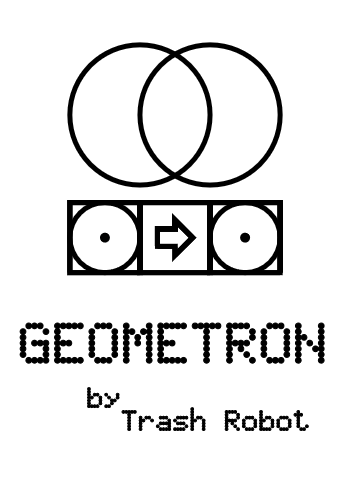
\includegraphics{cover.png}
\end{figure}

\clearpage

\clearpage

\thispagestyle{empty}
\mbox{}

\maketitle


%civilizations
%

\mainmatter

\chapter{Civilizations}


Dig it up, set it on fire, and bury it.  Our civilization is an ever-accelerating destructive flow of material from mine to landfill.  This work is based on the idea that we can do better. Much better!  We have dug such a vast array of useful minerals up in the last few hundred years and carried out such fantastic transformations on them into useful materials that we now have the opportunity to build a whole new civilization with a completely different structure than the one we presently inhabit.  

Our current industrial system is a tripod resting on these three legs: money, mining and property.  These ideas make up a philosophical framework for understanding and building our world which is failing at an ever-accelerating rate.  In order to build a new civilization, we must study in detail the structure of the existing one.  
  
Money as an idea is so integrated into our world view that it is very hard to even see what it is.  At its philosophical core, the idea of money is that there is a property we call ``value'' which can be denoted by a number.  This is considered so obviously true by defenders of the existing economic system that when challenged, they simply re-state repeatedly the basic ideas immediately assuming that any system not based on money is just the same set of ideas re-arranged. That is, people will argue that doing away with money will simply replace selling a things with a certain ``value'' denote by prices with trading things to which such a value can also be assigned, but just in a much more inconvenient way(barter). Similarly, the defenders of the idea of money will argue that ``storing value'' is an important task, again assuming that some kind of thing called ``value'' can be measured with numbers and that doing this all-important value storing will simply have to be done with vaults of metal if we dispense with money.  

But this monetary way of thinking does not take into account the possibility that the value of a thing might multiply by replication or that value can be created from nothing.  As long as everyone in society is exchanging value along this stream from landfill to mine, we can use the numbers we call ``money'' to roughly create an equivalent to the main type of value, which is physical material.  We can measure how much gold or cobalt or salt we have, and money lets us transform value from one of these physical things to another, easily trading lithium for silver or oil for aluminum.  

Furthermore, of course, there is labor.  In the labor theory of value, again, money is used to assign some fixed value to a certain amount of ``work'' people do to produce a thing. One can superficially dispense with money but as long as we accept that value comes from how many hours an actual worker one does some type of task, we are just shuffling the details around but preserving the structure.  But what of automation?  And what of other forms of even more drastic increases in efficiency which are possible with information technology? Again, once we allow for full automation and many orders of magnitude increases in efficiency, we find that there is no way to create a value system using numbers which actually describes reality as we experience it in an information economy.  Numerous band aids have been proposed, but if we project forward to more and more automation and further increases in efficiency we see that we have to re-evaluate the whole labor theory of ``value'' along with every other theory of value we hold as a truth today.  The problem, again, is that using numbers to denote value simply will never be compatible with the new civilization we must now build in order to survive.

What happens when we create value from something we have an effectively infinite amount of but which we only have a finite need for?  What if, for instance, I live near a landfill with a vast store of plastic and electronic trash, and I want to build a small factory which converts plastic trash into useful furniture for direct use near the material I have.  Suppose the electronics trash has all the material I need to build this fully automated factory, and that the material needed to create so much great furniture that no one near me ever has to buy furniture again, that they can get custom high quality furniture which can be repaired indefinitely without even tapping too deeply into the vast store of plastic trash available directly in our community.  This act of creation brings a thing of great value into being from nothing but information.  In this situation, money fails.  As long as we rely on money to denote and store value, everyone creating value from nothing has to either get someone in the money-creating business to create currency specifically for them or to do that themselves as they create.  

But the more creative our new industrial processes are, the more catastrophically the money system fails.  If I share the information on how to build the thing with the rest of the world, in principle the equivalent of trillions of dollars of value can be created from nothing. 

This failure is not hypothetical.  Creating value from nothing which can self-replicate freely is precisely what software does.  Software produces things of great value with no material input needed at all, and is able to almost instantly replicate to the whole of humanity.  If someone can create almost infinite value with no input of labor, energy or materials(after the initial creation process), what does that imply for the rest of the people?  We are seeing this every day.  Every city in the world right now is witnessing a violent takeover by the replicators.  Those who can replicate their products infinitely for free include the media industry, marketing, software, finance, and all the numerous information based businesses which make up those business ecosystems.  We are finding that at an ever-accelerating rate all the wealth in our society is being transferred from people who produce things that do not replicate, like physical goods or physical labor to the replicators. 

The purpose of the work here is to show that there is another way.  We can create an information based economy made up of self-replicating information which reproduces things of value which cannot be added up using numbers.  This is not some crude replacement for money using barter, but rather a whole new approach to everything: we will have to build a new way of thinking about machines, society, mathematics, and philosophy.  Just as the existing system is based at its deepest level on numbers, we propose basing our entire civilization on geometry.  Geometron is a universal geometric language which we can use to express the self-replicating information we will need to build this new civilization.  

The second leg of our tripod of civilization is property.  As with money, the idea of property is very difficult to examine as it is so deeply woven into the fabric of everything we do.  The world view we are taught in school and at home is that just as everything has a price that everything is owned by someone.  In some cases that ownership might be the state or even some type of ``common property'' but all things are in some way property.   In the dominant ideology of our time, air and water are property, the land is property, the genes in our DNA patented by the drug companies are property, and even these words I am typing are property.  

Again, as with money, we have to examine how this idea is going to fail more and more catastrophically as we evolve into a civilization based on the replication of technology from trash rather than consumption of mined materials using labor.  In many ways the purpose of property is to inhibit replication.  In the case of intellectual property this is in fact its \emph{only} purpose. But even for physical property like land, the whole idea is that if I ``own'' land the real purpose of that ownership is to make sure someone else does not own it. 

The idea of property makes sense when we are all competing for resources we have to dig up out of the ground.  If I dig up 1 ton of silver it means you can't and vice versa.  We are all in competition to be the owner of that silver.  If you are 1000 pounds of silver richer, I'm 1000 pounds of silver poorer.  But we have to see that with an informational economy based on trash as the main input this is no longer the case.  

If I consume a ton of trash from a landfill into useful things, we have to recognize that that ton of trash has a negative value, which changes completely what it means to use it to make things.  If I consume 1000 pounds of oil to make a plastic part, that oil has a cost we now measure in money I have to spend to buy the oil.  But if I consume that from a landfill, the cost is negative!  Regardless of what I make from the plastic, simply having it be something useful at all is of value.  In our existing consumer economy we all actually have to spend money to dispose of waste.  So an economy built entirely on waste streams breaks the whole idea of property up.  If I have a pile of trash on my land and you take it away that has value to me and also to you.  We are no longer in competition in this relationship--the more trash you take the more benefit I get but also the more you get.  

We must also recognize how an economy based on the replication of technology from trash using free information technology changes the incentives in regards to intellectual property.  If I create a new technology now and release it into the world, the only way for me to make money on it is to retain some control, which is now expressed by means of the property system. But if I create a new technology from trash which does something useful, and it's intended to only be used locally, the value proposition changes.  I use local materials to make a thing and directly benefit from it.  When I share it with you, you also do that, but if you then improve upon it and release it back into the network, I can immediately benefit from the improvement.  

If we build feedback loops across a global network we can get exponential speedups of technological development.  What this means is that if I am a technology creator and share my creations freely, the thing I create can be instantly transformed into a thing co-created by a global community which is vastly superior to what I would have made alone.  If my only goal in building technology is to directly convert the trash in my physical environment into useful things, my choices in regards to how I relate to the rest of the world will be based on trying to do that better and better.  If the more I share the more this happens, often with what I make being totally replaced by something much better, my incentives undergo a radical shift.  What I now want more than making a good thing and controlling it is making a thing which entices others to improve it.  Again, as with money, we find that the idea of property inhibits us from doing what we need to do to build this new civilization.  

The third leg of our tripod is mining.  This is perhaps the most fundamental.  The entire basis of our long strange trip from stone tools to bronze to iron to steel to silicon and so on is based on mining.  We need mines to get the materials to make things.   In order to make complex things with many materials, we need a global system which maintains physical control over all those mines using the system of property and the governments which uphold that property.  We also need a global supply chain again based on stability of governments and large institutions to maintain the constant global flow of goods.  In order for our current system to work, every individual element from oil to lithium to uranium must be transported to everyplace on Earth.  Conversely, every piece of land with a resource on it will under the current system be pressured to extract that resource and push it out into the global economy.  

Under the mining regime, every single type of mine is a choke point to the whole global system.  This regime is inherently conservative: any threat to any part of it will make the whole system fail, harming everyone who relies on it which is presently everyone.  In order to keep the system running, therefore, a constant global regime of military force is required.  One cannot have a mining based civilization without military empires to control the large scale flow of materials.  

And again as with money and property we have to examine how the system of mining affects our relations with our fellow people.  As long as value all comes from a mine, we are all in competition at some level for the mines products.  Every so-called ``developing'' nation will be forced by the dominant powers to extract all their resources to benefit someone else since all the nations are in competition to benefit from those resources.  

But when we build everything in our civilization from the trash of the old world this situation completely changes.  My motivation as a producer of technology is now to turn trash into things of value as much as possible.  If you are thousands of miles away, and we never exchange any physical goods, just information, my incentive is now to have you replicate the trash technology as much as possible.  This is for several reasons. First, there is the same reason as stated above in the discussion of property: the network effect.  The more people copy my technology the better it will get, and the more comfortable my own life will become.  But also, if we build a society which abolishes the mine,  as long as other people are mining they will pose a threat to us.  As long as anyone in the world bases their civilization on mining, they will need to build empires and dominate large masses of land in order to keep mining.  So if I want to not be invaded by a mine-based empire it is in my best interest to help every other place on Earth develop the same technology in order to also prevent the violence of the mine from destroying what we build.

In today's world \emph{every} single useful material we need for advanced technology has been pretty evenly distributed to every corner of the globe.  This is totally unprecedented! There is nothing in history even remotely similar to the situation we find ourselves in today.  People do not seem to have really grasped how fundamental and irreversible this is. Even if humanity died out tomorrow and were replaced by evolved crows in 100 million years, the distribution of rare minerals around the globe will remain.  We will never again have to discover from scratch how to find and extract materials like cobalt or tantalum.  We not only have all the materials needed to build an advanced technological civilization from scratch, those materials are already in a very organized form specifically designed to be useful.  Aluminum has already been extracted from bauxite, iron has been smelted into steel, silicon purified into wafers of unimaginable perfection and so on.  

Examining all three of these legs(money, property and mining) it should now be clear that these ways of thinking fall apart when we build all of our technology from trash instead of mined materials.  It is my intent in this work to build a framework for creating this new world.  To do this, we will need to build up a whole world of thought and action from scratch.  The most fundamental focus of this new world is replication.  We study how media replicates, how machines replicate, how software and hardware replicate, how whole systems replicate, and how pure information replicates.  

We also take as an axiom that geometric thinking is more fundamental than numerical.  This is because geometry is what we use to actually make things.  From buildings to microchips to injection molded plastic enclosures, all technology is essentially a geometric construction of one kind or another.  So if we are interested in building media the sole purpose of which is to replicate technology effectively, we find that geometry is the most fundamental form of mathematical thinking.  As with the existing system of thought we currently live in, we will need to delve deeply into our most fundamental assumptions of how the world works.  But now rather than trying to find some abstract truth, as the mathematicians of the early 20th century did, we build up a system of thought based on outcome: that which freely replicates useful things from trash is the goal, whatever that turns out to be.  This will lead to re-evaluating how we think about machines and mathematical philosophy, replacing the theories of ``computers'' with ideas about geometric machines to print symbols.  

One final note to make about this geometric world view.  As with all our mathematics in this new civilization, our goal is replication, not finding some higher truth.  This means that geometry is all based on its meaning to humans.  Even if the meaning is in the angle of a turbine blade which communicates a different level of air movement in an air conditioner, it is this meaning we care about, not some abstract theorem to prove or algorithm to own.  We therefore take language and symbols to be the most fundamental elements of which our Universe is constructed.  We accept that whatever we may think or do, the ``real'' universe is separated from our minds by a veil of language we can never fully see clearly through.  Reductionist science has made the mistake of ignoring this veil and focusing on a hypothetical ``objective reality''.  Whether or not this is a permanent intellectual dead end is of no interest to us here. We want results, fast. We want a better civilization in our lifetimes.  And to do that we build up a new way of thinking about information where our desire to provide direct value to people and replicating that to as many people as possible is our most fundamental axiom.

We call this geometric system of value, this geometric meta-langauge, Geometron.  This is the Book of Geometron, which describes how to replicate the whole system.

To build this world we will first discuss how media needs to change to support this new way of thinking, then how we will physically deploy this media infrastructure to the streets of our world.  We then show how the software works, how it replicates, and how you can add to it, improve it and make it your own to share.  After that, we step through all the different layers of information that make up this new network.  We then talk about our theory of being(ontology), the new underlying mathematical philosophy which we are using to replace the axiomatic set theory that 20th century mathematicians used to describe reality, as well as the theory of machines which replaces the Turing model of computation.  Finally we use this idea of how information works to discuss the self-replicating set known as Trash Robot which we will replicate through the network and also use as a vehicle to help stimulate replication.  

\begin{figure}
	\centering
	
\includegraphics[width=3in]{figures/shapes/blank.png}
\end{figure}
\begin{figure}
	\centering
	
\includegraphics[width=3in]{figures/shapes/blank.png}
\end{figure}

\chapter{Organic Media}

In a consumption-based civilization the purpose of all media is to stimulate consumption.  This can come in the form of advertising, corporate propaganda, or the legitimization of the imperial power required to keep mines and long distance supply chains operating.  In the age of digital media we find that the hardware itself is also a large component of how it facilitates consumption, with planned obsolescence creating a stream from mine to landfill unprecedented in human history.  A constant race to build ever more exotic materials and technologies into physical media devices creates a vast suction across the planet, forcing every corner of the globe to exploit anything that can be mined for digital media hardware from cobalt to lithium to be exploited as fast and widely as possible.  

This state of affairs creates a powerful opportunity for a new type of media.  The fact that the existing system pumps out this constant stream of new objects with all the stuff needed for advanced information technology creates a resource which can be used to build new hybrid technologies designed to incorporate scavenged parts from the discarded tech.  The tech industry is now working on turning out \emph{trillions} of ``internet of things'' devices--objects which have built-in networking capability and could in theory serve as web servers.  Based on how these industries are structured we know that these will all be designed to fail on a very short time scale, and what they are selling today will be in a landfill in less than 5 years.  

It is worth marveling at the scale of consumption built into the current digital media system before discussing the alternative.  People walk around with screens in their pockets, the sole purpose of which is to manipulate them into consuming more.  Those screens are built on a technology which uses the most exotic materials known to humanity, extracted at great human cost from every corner of the globe.  And then they are forced into obsolescence within months in some cases by a software industry which is based around the idea of planned obsolescence.   Having pushed their way into the pockets, homes and workplaces of something like half the humans on Earth, the industry is now pushing to put their devices in things which have no reason to be part of this network, like toasters and juice makers.  The sheer insanity of this is hard to wrap ones head around, but because the entire media is controlled by this industry it is hard to even articulate in public how insane this is.  And it is getting worse very quickly.  The need to replace this parasitic monster with media which serves the needs of humanity could not be more urgent!

What we want from a media technology to build  our new trash-based civilization on is to replace consumption with replication.  We are now constantly buying new machines built from mined materials which constantly tell us to consume more things.  Consumption-based media forms a consumption information loop.  We want to form a replication-based loop, where the media is built from trash and contains the information required to replicate itself.  We call this ``organic media'', because it behaves like a living thing.  In fact it effectively \emph{is} a living thing.  If we built closed loop systems in which humanity is re-using material again and again forever in order to live in harmony with the world around us, it makes sense to think of us in combination with our media and the ecosystems we live in as a living system.  

This idea of ``organic'' media is in direct contrast to ``viral'' media which dominates in social media today.  In viral media, information replicates, just as viruses replicate themselves inside a living organism, but the this is always happening in a space defined by a fixed media entity.  Social media platforms encourage information to replicate as fast as possible within their systems, as that costs them nothing and induces more people to keep coming back to their platform to be manipulated by their advertisers.  But if someone tries to replicate the media platform itself by for instance trying to start a new platform, they will do anything they can to stop them.  Media today can be viewed in biological terms as an apex predator which kills everything in the rest of the ecosystem and is full of viruses.  

When we say we want media to be organic what we mean is that we want the media platform itself to replicate.  Just as each new tree or squirrel in a forest really is a whole new instance of ``tree'' or ``squirrel'', with no central entity controlling them, we want each new instance of our system to be self-contained.  We want it to be able to replicate itself right where it stands, with no outside input from some central system of any kind.  This is only possible because of the waste of the existing industrial system: all the materials needed for advanced information technology are sitting in trash bins, dumpsters, closets, and landfills within walking distance of wherever you are reading this right now.  All you need to build a whole new media ecosystem from scratch is information: the information required to gather the people and materials required to build it.  If the system you build tells people how to do this, it can freely replicate across the whole world without any central infrastructure.  

It is worth noting that building this is hard. Modern digital media technology is designed by hostile engineers to be as hard as possible to fix, modify, or use for anything other than consuming advertising for a few months before it goes to the landfill.  Those machines are built by vast teams of well funded groups with extremely specialized technical skills.  It will take a concerted research effort to fully replace the existing information technology system with a free one built from trash.  In a later chapter, I will discuss how we can do this by using a different system architecture in which the purpose of the whole system is displaying of a specific class of documents based on the software presented here.   But for the time being, in order to launch our new media system, we will rely on existing off the shelf hardware which is still part of the consumer system but not the main commercial advertising-driven part.  

This book is therefore doing two things in regards to launching this system.  It is launching a new social media platform based on using the Raspberry Pi as a local web server used over local wifi networks, and it is laying the conceptual framework for building a whole new information technology system from the ground up on new principles.  Just as technology people in the existing system refer to a ``technology stack'' we are building a whole new ``stack'' in the sense of a collection of technologies which are all related by a chain of increasing or decreasing abstraction or proximity to the user which work together to make our system work.  In this work, we describe the whole stack.  We launch fully functioning software and hardware for parts of it, and describe how we will build the other parts that require more work.  

The most important part of the current project presented here is that it work for its purpose which will support the rest of the development.   This means that the technology has to work to distribute new technology of all kinds built from trash which people need or want, which can be freely replicated.  We use this partially consumption driven media system to launch self-replicating media systems which really are built from trash as a demonstration.  Our metric of success will be how this self-replicating media technology replicates and evolves.  If we can make it replicate by making things people want, and make it evolve by creating a strong incentive for people to improve it, the system will naturally evolve into the one we need, which no longer requires any input from the mine-based system to function anymore.  

Just as a relatively small number of people a few hundred years ago sending each other letters built the basis of the current explosion of technology which led to the existing world order, we believe that a small number of people with new ideas today can build a much faster explosion of information which consumes the existing world of consumption and replaces it with locally closed loops of material in a single generation.  We also believe that this is of the utmost importance to do as quickly as possible.  The existing system is killing us.  It is destroying the natural world, needs constant warfare to function, and is increasingly driving anyone outside the technocratic elite into extreme poverty.  

So how do we actually build this ``organic media''?  We start by looking at living systems, both individual organisms and larger systems like forests.  The most fundamental thing life does is replicate.   This will probably get tedious for the reader, but replication is the thing this work will come back to with relentless repetition but that relentless repetition of replication is precisely what makes life work.  A living system is a system of thing which all also replicate.  Living systems replicate over all scales: forests replicate, but so does the RNA and DNA in each cell of each organism in the forest!  We will also build our systems this way: many components make up systems from tiny scraps of code or single cutouts of cardboard up through whole vast industrial fabrication systems, and we want \emph{all} of them replicating.  Again this is in direct contrast to the existing system in which small parts like shared memes on a platform are supposed to replicate but the company itself is designed around non-replication.  

Another property of life is that it is an independently evolving thing.  Because organisms have an independent life, they can change in much more unpredictable ways than centrally controlled systems like a large corporation, government or non profit(this includes open source software projects with a central code base that all instances are copied from).  

Finally, all life dies.  In order for life to work we need the cycle of death to be natural.  Just as fungi in a forest turn logs into soil we need the destruction of all things in our system to be natural.  This is again in direct contrast to the existing system in which all media is built out of a company which is designed to grow forever and never die. 

In order to build our platform then we want to write down a set of rules which will guide all of our work.  These are nine rules:

\textbf{Everything replicates.} This is the most fundamental law.  It is what makes life alive.  And it is what makes media organic rather than viral or parasitic.  This means that all our software contains code to replicate itself without any reference to a central code repository.  The code on a server in a coffee shop can directly replicate to the laptop or phone of every person in that coffee shop with no connection to the rest of the Internet at all.  All our hardware is built into some kind of media which describes its replication.  

\textbf{Everything evolves.}  All things can be edited by all users.  To be in contact with a thing, be it a file or a physical machine is to have the power to alter that thing totally.  There are no ``users'' or ``engineers'' in the sense used today.  Some people will choose to edit things more than others but everyone \emph{can} edit all things.

\textbf{Everything dies.}  All things can be deleted or destroyed by all people.  This is particularly important for files.  Much of the power structure we are trying to destroy rests on information we are not allowed to destroy, from the intrusive and parasitic industry of buying and selling personal data through the constant advertising we are not allowed to turn off.  Also, in order to be able to stop harmful information, we empower every single user with no exception to be able to delete every single piece of information they come into contact with, with no exceptions. This is less destructive than it sounds. Because our network is all physically local, no central bad actor can wipe out the whole network.  If all networking is at the level of a wifi network, and they are all constantly being destroyed and rebuilt anyway, the cost of universal destructive power is outweighed by the benefit of people being able to stop bad information without any appeal to authority. 

\textbf{No property.}  As discussed in the previous chapter, the idea of property is not compatible with a civilization based on self-replication.  Since the idea of property fails at scale in a replication society, and since our goal is to scale, we dispense with it immediately and build infrastructure which not only has no intellectual property but where the physical web servers are not owned by anyone.  Initially we will have to spend money to buy parts to build them, but as soon as they are built we will release them to whoever we think will get the most use from them, along with instructions for them to do the same, passing all infrastructure along to wherever it gets the most use.  Building network infrastructure without property for the benefit of our communities means that our incentives are now to find whoever has the most need, identifying their needs, and using our technology to serve those needs and fast and directly as possible.  If people benefit from the systems, they will naturally be able to replicate, which will further replicate the non-property technology.  Initially this means building Raspberry Pi based web servers and giving them away to the people with the greatest need.

\textbf{No money.}  This is connected to the rule against property.  Initially of course we will need to spend money to buy parts, and will need to have users make money to support their near-term survival.  But as we scale up and get more and more basic needs satisfied by technology built from trash, we want to have the elimination of money be the direction we are headed from the start.  This is not as far fetched as it sounds.  As will be discussed in the next section, barter will be an incredibly powerful tool for scaling.  Our network can provide huge benefit to very powerful and wealthy people, and if our people with the most need are dispensing this benefit, we will be able to barter the things we need to scale directly.  When our network helps a business with a lot of unused space to make money, they can let us use their space.  When a business person makes connections using our network which make them money, letting us scale our software up on some of their servers will make economic sense to them.  We will be able to barter our value as network builders into the things we need for personal survival like places to sleep and food but also the things we need to scale our technology like access to labs and machines.

\textbf{No mining.}  Our long term goal is the global elimination of all mining.  This includes the whole natural resource extraction industry such as oil and gas as well.  This cannot happen overnight, but we don't need it to.  Every single mined component we replace with one from a dumpster or landfill takes a little bit of energy and power out of the mining system. if we can remove power from them in a way which self-replicates, our system will simply consume theirs, and mining will be eliminated in a generation.

\textbf{Everything is physical.}  This is almost a circular statement.  What does it mean for a thing to be ``not physical''?  This is a statement of belief.  We emph{believe} that the idea of information which is not physical is meaningless.  All information has a physical manifestation, be it charge on a transistor or bumps on a CD.  This law is important as a vocal rejection of any theory of how machines works which states that information or data can exist independently of its physical existence.

\textbf{Everything is recursive.}  One of the most notable properties of life is its constant self-referencing.  Billions of DNA strands in each individual body of a large organism all contain a whole copy of the information required to replicate the organism.  We see information which points to information which points to information.  Life is very self-referential and involves in an abstract sense functions which call themselves constantly.  RNA stores instructions to make molecules which replicate RNA, and so on.   This law is to remind us as creators of technology to be \emph{constantly} thinking of ways to make things point back to themselves to replicate. 

\textbf{Everything is fractal.}  This is another property of living systems that we take for granted but which we either ignore or make very crude imitations of presently.  Centralized systems of control create technologies which are flat in scale: we build microchips with nanometer precision across millions of nanometers(mm) of scale and so on.  In contrast, living systems are fractal in scale such the scale of ``error'' required to cause catastrophic failure scales with the size of the system.  We assume that patterns will repeat again and again at different scales, and expect that our technologies only need to be precise at the correct scale for any given sub-system.  This has very specific implications for fabrication which will be explored elsewhere, but as a law we mean that we must simply always have ideas of the fractal nature of living systems in our minds as we create new things in our new trash-based civilization.


With our goals and laws of operation stated, we are now finally ready to delve into more detail into what we are actually constructing with this work.  This is a local network based on a web server loaded on a Raspberry Pi.  The Raspberry Pi is a computer on a circuit board about the size of a deck of cards which typically costs about \$50.  It needs some peripherals including a screen, keyboard, mouse, battery, and memory card, all of which makes it about \$200 for a nice, easy-to-use, portable and self-contained system.  It only requires a few commands which are easily copy/pasted to install the whole functioning Geometron system on a new Raspberry Pi.  It is also modular, and if portability is not needed it can plug into the wall, borrow a keyboard from another system temporarily, and display on a TV, making a non-portable system cost just the value of the board(\$50).  

It is also important to note that this is all modular, easy to buy from many sources, and involves parts many people already have lying around.  The Raspberry Pi is widely marketed as a hobby tool and a STEM education tool, but its use case is not always clear.  Therefore a large number of people own them but do not use them.  They are often sitting in drawers in someones home office or a under-used maker space gathering dust.  If we have a use for them and can provide useful services to people it should be possible to directly barter with people who want to support our network who will be willing to donate the Pi boards to our network, where they will become non-property and be distributed to those in need.

The actual software we run on the Pi is what is described in the bulk of this book.  It is all designed to run in a web browser. Any web browser.  So if a Raspberry Pi running the Geometron server software is on a wifi network, all the programs and documents on it can be read, used, edited, replicated and deleted by anyone connecting to that wifi network on any device be it a phone, laptop, tablet, or another Raspberry Pi.  Also, the pi itself can serve be used in the same way as any other device on the network.  

We must also note an important condition for the pi to be a non-property computer.  In order for the pi to be able to freely be shared among the people, it cannot have any personal data on it which causes someone loss if it is read by another person.  That means we must never log into private networks like gmail, facebook, or more sensitive things like bank accounts ever on the system.  In order for a free and open system without property to function, it must be kept separate from the property based networks.  This media platform exists for the sole purpose of free sharing of documents.  Any document we do not wish to share we do not put on it. 

Also, there are no ``users'' on this network.  This is a network of documents, not users.  There are no logins, no passwords, and no databases.  User data is not harvested for profit because we simply do not generate the type of information which is considered ``user data'' in the existing systems.  

We take as an axiom in the development of this system that documents intended for free sharing are of greater value than private documents, and that the network effect as the universe of non-property documents grows will exponentially increase their value to people until our network out-replicates the existing ones.

Our network is based on sharing several specific types of document which are encoded into the software.  We share ``scrolls'' which are text documents, ``maps'' which are like presentation slides or memes, ``feeds'' which are essentially lists of information, self-replicating applications of all kinds(using web based code that runs in a browser, never native code), and generalized Symbols using the Geometron geometric programming language which takes up much of this book.  Taken together, these systems of document creation and replication will allow us to describe and replicate any technology of any kind.  

This network will be distributed physically, over the Street Network described in the
 next section.  We will initially try to get servers to people who are on the move, living on the streets or in vans and buses, truck drivers, street performers--anyone who finds themselves in nodes of physical networking like dense urban areas or truck stops with many people passing through.  The details of how to replicate the server are in the section after next, which delves into the code.  Not everyone will need to read this, but everyone should know where to find it, as part of what we will be bartering for as we scale is help from technical experts who can learn the system and replicate the software as well as add to it to evolve it and decentralize the code base. 

The rest of this book describes how to replicate the system, how to use it, how it works, how to develop it into a fully trash-based system, and how we will rebuild mathematics to support this venture.  

\subsection{The Book of Geometron}

This book itself is organic media. It is intended to teach its contents to a reader(or rather a small subset of readers) to the level where they can then teach another.  This should enable them to re-write future improved versions.  In this section I describe how the book was put together, where the files are stored, how to edit them and use the \LaTeX document preparation system to make the files required to produce a finished book.  This means you also need to know what is required to get the physical book printed at an on demand printer, get all the metadata required for publication and distribution, and sell your version in retailers both large and small and online and off.  Thus even the book is fully decentralized in principle: if it costs you nothing to set it up to sell, you can sell only a half dozen copies and it will be a net positive, and then if the next person does this it will also be positive and so on.

If the book is decentralized in this way of distribution it has many advantages.  If the book turns out to be disruptive enough that people try to use lawsuits to shut it down or harass an author, but there are 10's of thousands of new authors popping up all the time, it will be impossible to shut down. As some versions turn out to be dangerous or illegal, other versions can immediately be published with omit the offending content. Also, many editions will mean some will get much better than this initial manuscript.  Decentralization means that as the manuscript finds its way into communities that speak different languages, the translation can happen without any centralized effort. So for instance if someone translates from the original English into say French, and then it spreads around in areas bilingual with French and some other language like Swahili it can go directly from the French to the Swahili without any involvement of the initial English speaking writers.  By avoiding copyright, these improved and translated versions can then get translated back into English and sold yet again under yet anotehr edition.  Having editions be unique can create a market for unusual editions, further pumping money into the system and stimulating further development of the book.  I would rather see 10,000 people make 100 dollars each selling their own editions of this book to just their friends than see me as the initial author make 1 million dollars on 500,000 copies of one edition.

It is not my intent in the long run to make money on Geometron. It is my intent to create a network which allows us to live without money by directly bartering what we need to survive(food, a place to sleep and work, medicine, transport) without use of money or any production in the old consumer economy.

All editions are published with a public domain license for everything but the final pdf.  The final pdf is published under the minimal copyright required for an author to create the needed publication metadata to get distribution outside of the on demand press used for printing.

Each chapter is a .tex file, using standard \LaTeX.

This work must replicate itself completely.  We show here how to edit each chapter, publish them to a public Github repository with detailed instructions for further replication, compile the document to a .pdf in book format, and self-publish the fully compiled book on Lulu Press. We then guide the reader to follow the instructions on Lulu to get all the needed copyright metadata for official distribution through normal publication channels.  We then describe how to order just a few copies, sell them along with other parts of the system here at a markup, and use the profits to buy more print copies of their own book to place in bookstores and libraries as a fully guerilla activity with no official sanction.  This is a little twist on the methodology of Abbie Hoffman's ``Steal This Book.''  In Steel This Book, book sellers had to buy the book, which readers inevitably stole, cutting into book store profits.  We use guerilla production methods to distribute it into bookstores without them spending money.  They are faced with a choice: go along with our program and take free money from customers for the book or make trouble for us, throw the book out, and loose what is for them totally free money.  If they sell the books for a profit, it benefits our network, because it spreads our ideas but also because it creates a value stream in the existing economy based on what we create, which gives us power in that network.   Bookstores want money.  But we want network centrality and the ability to control how information flows in a network, and free distribution shifts the power to us.  This is why the self-replication of the book is so important.  If you want to make your own spin on this book and make it more of a best seller, you do it, but if you leave it open, you hope someone else does it again, and that it keeps getting better as it replicates.  Replication instructions for the physical book will live in the README file for the book repository on Github.

Another way to make the book self-replicating is to distribute print copies which a number of blank pages, sold at cost.  Artists can buy these, then create illuminated manuscripts with custom illustrations of geometric art using Geoemetron.  This can then be bartered based on the needs and powers of the artist, with outcomes as diverse as the artists themselves.  We can use this to barter for what we need to expand the network, to survive, and just as another way for artists to exist and thrive in the world.  Also, this can be passed along and shared as non-property.  You can buy the hardcopy of the book, add a little art, and pass it along, then the next person adds some and passes it along, and we all help each other out along the way.  A famous artist or tech creator might be able to barter for something of very high value.  Each physical work will be unique.  And since the electronic files which generate the pdf which goes to the hard copy also self-replicate, this entire system can evolve and replicate, as dedicated creators rewrite the whole manuscript and add their version on Lulu press for sale at cost print-on-demand as well, and so on.
\chapter{Street Network}

\section{Street Network}



outline:
\begin{itemize}
  \item
  what and Why?  The power of the physical, local, and free.  Organic media, what we want, links to previous chapter.  Universal social media for sharing of information in a physically local domain with both content creation and consumption on all Web-enabled devices(laptops, phones, tablets, etc.)  Hybrid markets: like Craigslist, but way more local.  General description of what the system does(scrolls,maps, feeds, symbols, apps, industrial design and production via Trash Robot). This points to the subsequent chapters about these actual things.  Free boxes and food not bombs.  We are a hybrid between free boxes and food not bombs and craigslist.
  \item
  The Terminal.  This is the heart of this system. What is the Raspberry Pi, why is it powerful?  How to build the Terminal. Options involving big screens and projectors, public terminals with large publicly viewable displays.  How to adapt it to different situations, how to work with wifi networks, IP addresses, local and global, opening up a local wifi to a public domain.  how to avoid ANY property.  How the terminal is passed from user to user to operator to operator.  Data hygiene: how to keep all personal information of any kind of the machine, to prevent leaks of property.  What it means to have a network without property.  Replication paths via local laptops(localhost) on wifi, global github repos, replication to global hosted domains. How to constantly back up and replicate to avoid information death.  How to kill bad information.  How to nuke the whole system if it's too rotten.  Grey market and black market commerce.
  \item
  The Operators, what we are, what we do, how we do it, how we make money and barter, how we train new Operators .  Role of Operator as universal moderator.  Forking and avoiding the trap of the network monopolist.  How to transition between money to barter, how to scale up to an all barter system by providing value for 
  \item
  Psychogeography.  Nodes of power, examples at global level and local level, finding the nodal points.  Go through the whole philosophy, places, examples such as: parks, intersections, neighborhoods, famous landmarks, bridges, forking below a place, discussion of distance scales and granularity.  Targeting nodes of power: Sand Hill Road. Wall Street. SoMa.  K Street DC. Jackson Hole. Martha's Vinyard.  Navy Memorial DC. Use of power nodes to build extremely powerful local networks, where information is exchanged between players in existing power networks.  A network in the right coffee shop could connect people who collectively are processing 10's of billions of dollars of commerce just in that one coffee shop!
  \item
  domains.  choosing domains, buying them, sharing them, avoiding troubles. Entropy of domain choice, size of name space. use of free web hosting services.  Signs, markers, stencils, postcards: physical media which points to domains which point to terminals and link to the IP addresses.  The work flow with physical media to software media and back.
  \item
  The market
  \item
  the coffee shop(or pub) node.  How it can build community in the coffee shop, help all coffee shop customers to share and prosper, help neighbors of coffee shop, the developer workflow, use to expand operators.  Coffee shop network as service for coffee shop owner for barter for coffee and food at shop.  Building collaboration with businesses, both local and global, how to use global chains to scale globally with mutual aid and benefit for all.
  \item
  scaling up: the global swarm, going to full stack geometron(see last chapter), building more 
\end{itemize}

\subsection{What is the Street Network?}

We want an information network based around physical replication of technology from trash.  To stimulate the replication of the Network, we need it to create value for people who use it and operate it. This value can be of many kinds: it can directly provide physical goods people need, it can facilitate business in the monetary economy, it can provide mutual aid to a community, it can create local social connections, can build network power for users, and any of these values can be traded for materials and space needed to continue to expand the network.  

Truly free network. The Humble Pi.  The power of a network without property or users.  Networked technology with free sharing can create more value for users than one with private data.  Destroy the data brokers by making a network with no personal data.   

This book will describe several products and services which Operators in the network can provide to local users.  These can be exchanged for money or bartered directly for materials to expand the system(for instance one can ask users who are paying for goods or services to simply buy more computer equipment to build out more network infrastructure.)  We aim to have the goods sold be as much as possible based on a stream of trash which are upcycled into sellable products.  The prototype product here is a purse, the ArtBox, which can be constructed using the methods of Geometron and which contains the tools to replicate itself.  It is, in essence, a self-replicating purse with a unique Open Brand, the Trash Robot Brand, which will be documented in its own chapter.  

Services rendered will generally be of the kind which makes money for the user.  So for instance a passerby might place an advertisement on a news scroll for a local coffee shop for their service which other coffee shop customers(this is all over the wifi network of the coffee shop so everyone is indeed a customer) might want.  This makes the user money, which motivates them to come back and place more ads, so they are making money which they can pay to the Operator.  All of this commerce then motivates people to come into the coffee shop and read and share documents.  Since wifi has a time limit and requires purchase, this brings higher traffic to the coffee shop, which then has their revenue go up, so to keep the system running, it is worth it to them to barter snacks and coffee to the Operator of the network.  

Structure and purpose of the network: domains, places, operators, mutual aid, markets, 

Networks are advertised with physical media which points to domains which point to physical places, specifically to the location of the physical web server, and have a hyperlink which only works on the local wifi network which links to the web server on that network.

The Street Network is social media based around physically local instances of the Web which are not on the public Internet.  Wifi networks are used to share documents locally with other users on the same network.  The Geometron servers function as public bulletin boards, where documents are shared freely with all other users. Any user can edit or delete any file. All files can be copied by anyone.  Documents are all visible by both mobile devices and computers, as long as they are on the same wifi network.  The Street Network is an example of Organic Media. It is intended to facilitate replication by users.  Users can create and share documents advertising whatever commerce they wish to engage in: they can sell things, share ideas, give things away for free, advertise services, advertise businesses, describe how to make things, or look for others with shared interests.  There are no users and no databases.  There is just a list of documents which users can click on to read, edit using the editors or delete using the file deletion tools.

The Geometron documents are stored on a Geometron Terminal, which is based on the Raspberry Pi mini-computer.  Raspberry Pi is a non profit project from the UK to create a minimalist Linux based computer, mostly for education, research, art, and maker hobbies.   They can be purchased easily online for approximately 50 US Dollars.  The two most widely used formats of Geometron documents are the Scroll and the Map.  A scroll is just a text file, with some formatting in a markup language called Markdown.

Add paragraph somewhere on role of cryptography in sharing encrypted plain text copy/pastable files.  add functionality.  PGP?  ask someone for help on this section to get it right. How does this all work with various crypto technologies?  free sharing of encrypted files which can be replicated but then decrypted privately.  This can be a huge vector of replication for the crypto community, including inside the formal and informal intelligence community.  

what does the server do, what is an app, what is a document, overview of symbols, maps, scrolls,data,apps,automation.

Edit scrolls.

Edit maps.

feeds.  using feeds.

Workflow, developers, apps.  reference code structure chapter. Coffee shop developer community.


\subsection{Users}

We are looking to build a network which promotes the development of physically local power structures.  To that end, we choose nodes of physical power, such as the most important locations in global cities like key traffic circles in Washington DC.  We then study \emph{all} the stakeholders in that physical location. This includes residents, tourists, people walking through, truckers, commuters, workers, panhandlers, local homeless, business owners, the local mail carrier--really everyone, but restricted entirely based on that physical place, rather than any other affiliation.  Our network seeks to give the power of networking in that place to everyone in that place. As more people join, more infrastructure is added, until an entire ecosystem of interconnected network nodes grows up in some cases around just a single street corner(say 16th and Mission for example in SF).   

The network has to start somewhere, however.  We start with Trash Robot, operating the robot to make and sell tokens, and selling all the parts of Trash Robot.  We can recruit people to learn the system who can immediately sell Trash Robot elements to make money, which will lead to replication of the network.  Since Trash Robot uses the Geometron system to design the symbols, share how to build the robot, program the robot, etc., the social media system will be automatically replicated as Trash Robot replicates.  If the network replicates and Trash Robot Operators learn to operate the Geometron servers, the network will grow, and like all networks its power and value will increase exponentially with size.  We also initially need developers to improve the code and build out the more technical elements of the system, essentially setting up Raspberry Pi based web servers and distributing them.  So initially we need two groups of people: people to build and sell the elements of Trash Robot and people to develop applications for the Geometron system, build servers and distribute and install them.  In both cases, Trash Robot builders and Developers can be recruiting Operators who have less specialized skills but can make money from the system via simple means of just stamping out more and more tokens from already-printed stamps or posting ads for people for money on a bulletin board they operate but did not set up.


Trash Robot Makers: build trash robots.
Trash Robot  printer Operators: run the robot to print.
Trash Robot artists: design new symbols
Trash Robot market Operators: operate a bulletin board



Geometron Developers.    Geometron Operators.


A Geometron station can have a huge display which all passerby can read without even loggin on, also.

In order for this network to grow it has to create value for people. The more people it provides value for and the more value it provides, the more effectively it will replicate.  I will now discuss some of the specific groups of people who can benefit, how they can use the network, and what the benefits are for them specifically.

Traveling kids, hobos, panhandlers, people asking for money or selling things on the street corner.  A physically local free bulletin board shared by passerby in a high traffic area can allow people asking for money who are currently ignored by passerby as just another anonymous face and cardboard sign a chance to really tell their stories and to share all that they have to share.  When people share their stories they can become part of the emergent physical community of passerby in a location where the network node is located.  When people view others as part of their community they not only are more willing to help, they can have open communication about the best way to help, expanding from just spare change to more comprehensive mutual aid.  Because we clone content from the local terminal to web pages on globally visible domains linked to a physical place, which are advertised everywhere in that place, marginalized people whose only ability to get online is the public library can use the computers there to get the information they need to better survive, and ultimately to thrive and build new communities where they already are.  The way a local network can help people is twofold. First, it is direct, by asking for money and other mutual aid.  But by being physically on location all the time, already with physical media(cardboard signs), people in a given place can aid the network, creating value for the other people in the community who are more resourced, who then no longer view monetary support as ``donation'', but rather as an expense which supports their other business activities.  

In order to see the power of this second means of network support of marginalized people on the street, we have to look more closely at the network nodes we are building.  One of the major types of node is in a business district of a city where there are both homeless people asking for money, on the street all day with physical media, and power brokers who make their living entirely from connections.  These people include venture capitalists, entrepreneurs, lobbyists, consultants, and the rest of what might be called the ``deal-making class''.  An example of this confluence is some of the parks along K-Street in Washington DC.  K Street and adjacent streets is home to a huge homeless population as well as power brokers whose livelihood depends entirely on connections.  If a physical network were built which facilitated direct communication between people along K Street, the people who spend the most time physically on the street can be brokers of information on a network which can be worth a lot to the people who trade in information.  Physically local information networks can leverage the power of physical places with very powerful people walking past all the time who normally never communicate.  Connecting these people up can be dangerous.  But if we provide them with value, it can be worth a both a lot of money to them and also potentially something they can barter for giving us space to live and work nearby.  If you facilitate a 10 million dollar deal and the customer knows you can do it again, the least they can do is give you a 100 dollar gift card to the nicest restaurant in the block.  There is no real upper limit on what an enterprising Network Operator could in theory make if they learned to really channel information efficiently in the nodes of global power.  And of course we must remember that when dealing with power brokers their currency is not money.  When the people who currently have the most power in society find themselves dependent on free open networks, those networks themselves will gain power which penetrates that of the existing power structures, potentially creating an existential threat to them.  We must take note of this.

The elements of traveler culture which overlap with ``van life'' are also key to increasing the network effects of the Street Network.  This also links to trucker networks.  People who live their lives on the road can use this network infrastructure to set up complex networks and markets in highway rest stops, Walmart parking lots etc. using either wifi networks in these places.  These networks can be of utility to passerby of all kinds, from tourists to truckers to the workers who keep the places running.  Just as existing global social media networks provide value they can charge money for, a physically local network can provide value which people will pay for.  An example use case here is a Street Network Operator agreeing to maintain a backup of and keep posting an advertisement for something a local entrepreneur is trying to sell to truckers.  In exchange for that, they can get directly compensated in gas, right there in the rest stop, without money changing hands.  


Food not bombs, street outreach, harm reduction people, mutual aid workers.  See above.  The people who are working to help the most marginalized members of any given community can better reach that community if there is a physically local media platform where people can share information about resources.  Documents can be posted which explain how to get access to resources, when and where resources will be available, etc.  Because the whole system self-replicates, as with Food Not Bombs, anything which is successful in any given place can be immediately cloned to other nodes on the network.  Food Not Bombs already has a global network of free and open nodes with no property but a very recognizable brand identity and set of behaviors and actions.  FNB nodes are generally already linked by networks both online and via people who travel from one punk house or FNB house to the next.  The whole anarchist network of community houses, FNB's, anarchist infoshops and bookstores, really really free markets, free boxes, etc. can form a basis for a truly free information network carried from house to house and city to city, running on house wifi networks.  

Coffee shop owners.  Building a network in a coffee shop on the wifi network which requires purchase to use and which has a time limit can create a huge amount of added business for any local business owner.  It also builds community. So coffee shop owners who find themselves with a full shop of laptop drones with headphones on who work for hours, or get kicked out and do the same thing somewhere else can instead find themselves the brokers in a very powerful information network.  Much of the commerce of the world is now code written in coffee shops on laptops.  Creating physically local networks around these already existing groups can create huge power for the users which then benefits the people who set up the infrastructure(again, just like existing centralized social media platforms.)

Developers.  We need developers to be constantly writing more and better software in order to make Geometron a success. Developers who work all day in coffee shops or any other shared space like a co-working space or pub can have a social network based on both co-developing applications useful to all and sharing other resources.  Developers will use the resource of the Street Network terminal/server on the local network in the same basic way as others: they can share their resumes, links to pages of personal projects.  Developers are key to the whole system. We must recruit developers with this book who will rewrite all the code and also the book, replicating the whole system.  The faster our network can get developers into the swarm, the faster the code itself will improve.  Developers are key!!  Developers create servers to share into the network.  

Power brokers. Venture capitalists, financiers, entrepreneurs, deal-makers of all kinds, lobbyists, politicians.  Your network is your power.  Geography matters.  Build a network in the lobby.  Post things on street nodes, build your network, build your power, build your literal street cred. Dealflow.  

Crafters, makers, jewelers, artists.  An alternative to Etsy, street vending, or being in a shop.  Post your stuff to the local networks.  This is much more free and long form than existing platforms, you can post images, descriptions, contact info, times and places when you'll be in a place.  This can be way easier than other sales channels for arts and crafts.  You can say when and where you'll be at a place, post a link for contact, and then show up in the network node like a coffee shop to make the physical exchange.  In many cases, because the network is physical and local, there will be barter opportunities as well as direct sales.  A barter economy can develop where people donate materials you use for your crafts as part of how they pay for the finished product.  Removing shipping or transport costs by dealing directly in a physical location removes friction from the market, amplifying dramatically the power of the market, especially for crafts which involve physically bulky objects.  For instance, people can bring in motors and properly prepared plastic sheets and cardboard, as well as rolls and rolls of duct tape, and we can exchange finished products built from these materials and tools, as well as free food, drinks, and supplies, creating a market economy without money as well as without formal business structures(making it easier for marginalized people to participate).

Any labor pool of gig economy workers focused on a specific geographic location.  The most obvious of these is the drivers who presently drive for the major rideshare apps who all congregate at the airport to pick passengers up in the same exact place, and yet all of it is currently coordinated via the apps(unless you do the cab line).  The rideshares apps have proven that cities will ignore illegal cabs if they're done at scale.  It would be straightforward for a small team of Network Operators to run a server which replicates to a page which is advertised around, something like a domain of yourairportnamerides.xyz, which tells users how to log onto the wifi network created by an Operator's hotspot near the pickup zone and with a link on the page to the local network address of the server.  All all this IT is doing is directing customers to a dispatcher who manages the drivers over a simple app shared by the collective.  The whole network is run by a team of about 2-4 people.  One person might be a developer, who creates the app to manage all the drivers and post messages from dispatch.  Another person is all marketing, putting up the relevant information in the right places to get seen by travelers but not stopped by the rideshare apps, airport authorities, or the cab companies.  Riders will never have their destination information on the public network, nor will drivers put personal information, but they can work on an open trust model where they are known by dispatch, who has code names for them, and operates a queue app which simply adds drivers as the arrive near the Airport and pushes the most senior driver to the top of the stack, which is passed along to a rider.  Another Operator might be the one who runs the trust network for the drivers, verifying everyone and organizing meetings for the whole cooperative.  This can be used to unionize existing workforces quickly as well, building ad hoc networks which are very hard to suppress visible to everyone on their mobile devices on a local wifi network.  

The same model holds for places where workers congregate looking for short term construction work.  Those locations can have a server where an Operator runs a labor marketplace where a much larger and deeper labor pool can now advertise, but without all having to be in the physical location.  This means a crowd of a dozen workers looking for work can be replaced by an Operator with a sign pointing to the domain where the copy of the market is hosted.  Workers who come by can leave an ad on the local Raspberry Pi Geometron server, and anyone coming by looking for construction labor can just scroll through a now much deeper collection of ads and call whoever they need to hire.  A market place like this can suddenly go from a dozen general laborers to a construction labor market which includes specialists like plumbers and electricians as well as much larger general contractors just looking to save on marketing costs.  A person holding a cardboard sign on a street corner by a giant box home improvement store can now potentially be the broker of an information network on which millions of dollars of commerce flow.  


Trash Robot.  Trash robot will be described later in this work.  It is a system of technology which can be used to build products from a combination of waste streams and consumer off the shelf(COTS) products, which has a clearly recognizable brand identity owned by no one and provides value to an end consumer.  Trash Robot is a meta-business: a system for people to build businesses which can use both barter and sales to make money on the Geometron Street Network, further facilitating the replication of that network. If the right people start doing Trash Robot on the Network, we can create a system which has a significant consumer demand.  Trash Robot is structured to be very easy to replicate for an individual but very hard to replicate for a for profit centralized technology company driven by building up value in their equity.  This means if we can build up a significant consumer demand, it will provide a very powerful stimulus to replicating the nodes to grow our network, always as a free decentralized system.  Building a thing that replicates faster than property that is not property is how we start building a society without property.  This is described in detail it its own chapter later in this book.

Trash Robot is the most obvious way for those of us who are building this network to exist.  Other people might be Operators, developers, or participants in various markets, but the Trash Robot is the heart of the hardware development which this whole self-replicating social media platform is designed to replicate.  Trash robot is the reason we are building the Street Network and Geometron information system.  Trash Robot is a system of technology which provides value to people of a variety of kinds.  But because it allows Operators of the Trash Robot to be able to print nice clay tokens printed with arbitrary icons designed on the system, we have the ability to issue our own symbolic currency, which can create a new geometric economy not based on money but with some similarities.  We will build clothes with an open brand people can use to replicate their own copies.  We will make interesting or useful accessories like purses, machine carrying bags, and jewelry. We will make and sell robots, and teach classes on how to make them and use them.  And we will make the icon tokens to mean anything and exchange for anything. 

The tokens printed on the Trash Robot printer are totally unlike money.  They have no numerical value of any kind.  What they have is simply two symbols, both created in a universal geometric language which can be copy/pasted freely across the Network.  If someone sends you a text message with a string of numbers separated by commas and you give that to the Operator of a Trash Robot Icon Token Printer, they can just paste that text into their browser, use the code in there to program the Robot Printer and print the pattern into clay from the code. Also, the coins are all themselves self-replicating without the printer.  Because they have depressions along where they are printed, clay can be molded around the depressions to make another clay token which has the inverse of the pattern in it but with raised clay instead of depressed. When this piece of clay is baked, it can then be used to print another token, making an exact copy of the original.  This can be repeated many times. Thus printing one coin with a Trash Robot Printer can propagate out to in theory a very large number of copies.  Copies might degrade as more and more are made but if each copy is used to make many copies and so on, in a giant tree, one can easily imagine one print making thousands of tokens with no more use of the printer!  Again, we have made self-replicating media, both self-replicating online where we can share the code which does the print and self-replicating in the physical manifestation where the clay objects are used to make more clay objects.

\subsection{Building the Geometron Terminal/Server}

These should be called servers because they're servers.

Buy the stuff:

\begin{itemize}
\item
Raspberry Pi 4 board from Sunfounder
\item
SD card
\item
SD card reader
\item
Mini USB keyboard(without number pad)
\item
mouse
\item
Sunfounder HDMI display with 12 volt power supply and USB power out to drive PI, wall plug and HDMI cable, or similar display which can run off of a 12 volt barrel connector with a USB power output to drive the Pi.
\item
12 V LiPo battery pack with wall plug charger from TalentCell(sold via amazon)
\item
wifi hotspot
\end{itemize}

Put it together.  Just assemble the Sunfounder terminal as per the instructions.  

If you have a display that does not have a mount for the Pi, build an integrated terminal with cardboard, duct tape, and plastic HDPE sheet from milk bottles.

Burn the card with NOOBS, put it in the Pi.

Use paint pens to put symbols on keyboard.

plug in mouse and keyboard.

Make a bag to carry the terminal around in, or find an appropriate backpack and sew symbol onto it.  Symbol of Raspberry Pi using Penrose Tiles.

Boot up the pi, set it up with no password

Install Apache and php

copy the Geometron code replicator script replicator.php into the web directory. THis can be found from any geometron server at [serverurl]/php/replicator.txt.  

Learn to use with subsequent chapters of this book, customize and deploy, replicate to other people

run in headless mode, or on big screen, discuss display options, how to deploy in different places


\subsection{The Operators}
Building a relationship between Operators and Developers.  Operators deal with people and information.  Developers deal with code and build the apps to allow operators to operate. Operators connect people: passerby, shop owners, truckers, workers, drivers, developers, community members, other operators.  The Operator is like a switch board operator in the old Bell phone system before automated switching.  Switch board operators in small towns before automation knew not just phone numbers but the structure of the town, who was likely to be where, who gets called a lot, and in general how information flows through the networks of the town.  This role is very old, however and has been held by pub keepers, religious figures, coffee house owners, and numerous others throughout history and throughout the world.  The role of the information exchange manager is one all societies need.  The Geometron system creates a specific way for someone to carry out this role in a geographic location, which is easy to replicate in other locations, and to share information from place to place.

The relationship between Operator and Developer is key to structuring the network in a way that scales.  Both roles have to be self-replicating in that Operators recruit and train Operators as well as find new people to get trained as Operators


\subsection{Psychogeography}

Introduction, what is Psychogeography, the historical references to the situationists.  

Coffee shops and the laptop classes.

Global power nodes. examples.



\subsection{Domains}
\subsection{Street Market}
We help people sell stuff directly on the Street, out in the open, with a sign advertising the Market.  People can sell for barter.  We also sell directly the items from Trash Robot and other Geometron Things described below.  These include the ArtBox as a purse, shirts, pants, flags, bags, clay icon tokens, robots, terminals, laser cut acrylic shapes and rulers and protractors, Pyramids,.
\subsection{Coffee Shops and Pubs}



\subsection{Scaling Up}


Street Network:

\begin{itemize}
  \tightlist
  \item
  operators  
  \item
  terminals
  \item
  domains
  \item
  streets
  \item
  places
  \item
  developers
  \item
  signs
  \item 
  postcards
  \item
  markets
  \item
  feeds
  \item
  scrolls
  \item
  maps
  \item
  pages
  \item  
\end{itemize}






The \href{scrolls/terminal.md}{Terminal} is a
\href{https://www.raspberrypi.org/}{Raspberry Pi} with a keyboard,
mouse, display and power supply, which run a web server only visible
over the local wifi network. It is carried by the Operator, who uses it
to help users create, edit, copy, and share files over the local
network.

The files on the Network can be: - \href{scrolls/scrolls.md}{Scrolls}.
These are a type of text file which uses the
\href{https://daringfireball.net/projects/markdown/}{Markdown markup
language} for formatting.\\
- \href{scrolls/feeds.md}{Feeds}. Feeds are either a directory with a
sequence of files a user can scroll through and select or an array of
any kind of information, be it images, symbols, words, links, etc. -
\href{scrolls/maps.md}{Maps}. A map is a sort of generalized meme, like
a PowerPoint or Keynote slide. It is an array of elements each of which
has a position, angle, width, possibly an image url, some text, and
possibly a link destination, which might be either a HTML hyperlink or
an internal link to a file on the system

All users on the same wifi network as the Terminal can view, edit,
delete, and copy all the files on the system. There are no user names,
no logins, no passwords, no private data, and no databases.

Users can all see all files, edit them, delete them, copy/paste them,
create new ones

Operators carry the Terminal around, share its link with people, talk to
people about the system, teach users to use the system, help to share
with new Operators.

Roles of the Operator:

\begin{itemize}
\tightlist
\item
  the keeper of the physical Terminal
\item
  maintain relationships with users of the Terminal and Domain
\item
  update the Geometron server at the hosted Domain with links to the IP
  address on the local wifi network of the Terminal, as well as the wifi
  network name and password or link to where to get it(e.g.~coffee shop
  register)
\item
  post ads for money or barter on the Geometron server at the hosted
  Domain for people who ask
\item
  post on the global Geometron server when and where the Operator will
  appear, or where the terminal is set up on what network if it's
  installed permanently.
\item
  Teach anyone who wants to learn how to be an Operator, recruit new
  Operators
\item
  Tell new users about the Network, teach them to use it, how to post,
  edit, delete
\item
  Promote any kind of business or other venture or project anyone
  physically local to the wifi network area has in exchange for barter
  with that user for useful things on location(including just a place to
  operate)
\item
  Spread Network into new places by finding a location with a wifi
  network, buying a domain and setting up hosting or getting someone to
  do that and pay for it,
\item
  Domain names spread in physical space using physical media with
  depiction of domain which points back to terminal ip address, wifi
  address and password, photo of terminal and operator other physical
  media(post cards, book marks, spray paint stencils), spreading the
  physical media with the domain name
\end{itemize}

Skills of Operator

\subsection{Domains}\label{domains}

\subsection{Terminals}\label{terminals}

\subsection{Laptops}\label{laptops}

get ubuntu working under windows, install apache and php

localhost

code goes from terminal to laptop to github to

\chapter{Servers}

Servers are machines that store and share documents in the Geometron system.  There are three kinds of servers we work with: the Raspberry Pi servers that form the real backbone of the network, globally visible hosted domains used to point people to local Pi servers, and developer servers for editing and sharing new versions of the Geometron software itself.  

To spread the Network, the most fundamental form of replication is replicating the local Raspberry Pi server.  To do this, we want to either buy or barter for the parts, install the software, and teach someone how to operate it so that it can be sent out onto the Street for public use.  Given the choice, we will always barter for the parts.  If we can find people who support our cause and have extra technology hardware like old keyboards, screens, or even Raspberry Pi boards, it will be easiest to take direct donation of hardware on location by an existing server than to deal with purchasing and shipping new hardware.

The elements of the basic Raspberry Pi server are:

\begin{itemize}

\item The Raspberry Pi board itself.  This is a circuit board about the size of a deck of cards.  All of them should work! Older ones might be slower but they should all work.  This has all been tested on the Pi 3 and Pi 4.  Boards are generally between 40 and 50 dollars, but again if you can barter them that's ideal, as they are often sitting idle in peoples desk drawers.
\item micro SD card and SD card reader to write the card.  
\item USB keyboard.  If possible, find the one without the number pad so that it fits more easily in a backpack, this can make a huge difference in portability.
\item USB mouse.
\item HDMI Display. Not all work, but all can be made to work. Ideally you want a small screen which can run off the same battery as the Pi.  If you are setting up in a fixed location you can use any standard modern TV screen, which good both for needing fewer new resources and for visibility.  A large screen display for a server can be a great way to have shared physical social media, where people can read documents on the big screen without needing any device of their own.  For small portable ones we recommend buying ones specifically sold for the Pi, and which say that they don't need any special installation of software to work.
\item HDMI or HDMI mini cable.  There are some tiny Pi displays which don't need this because they connect to the pins on the board.  Note also that you will need the HDMI mini cable for the Pi model 4 but the regular HDMI for all other models.
\item Lithium ion polymer battery packs. This is only for portable installations, but it is important to have something modular and portable with a lot of power storage capacity.  We recommend the TalentCell batteries as being easy to charge, easy to carry, and having both 12 V and USB output.  They also sell solar chargers for those batteries, which are useful to have for long stretches of being away from power.
\item Wall power.  For the Pi model 3 and below this means a wall supply with the same USB micro and for the model 4 it is USB C.  You will want a wall supply that can put out 3 amps at 5 volts.  Also, if you are running everything of 12 volts you will already have a wall supply that came with the battery packs listed above.
\item Wifi hotspot.  This can just be a phone with the hotspot turned on.  But it can also be a mobile hotspot from the phone company which has its own wifi and connects to the network.

\end{itemize}
 
When you have all the materials to make a server, you will want to start by setting up the Raspberry Pi in the normal way documented on the Raspberry Pi website.  Follow the instructions on there to copy the NOOBS operating system onto the SD card.  You can also buy SD cards with NOOBS already installed.  The Raspberry Pi home page is www.raspberrypi.org.  Buying Raspberry Pi stuff can be done in person at some electronics retailers, some maker spaces, and online from numerous retailers, just search and look around.  Sunfounder is a great source of compact portable screens for the Pi as well as other Pi things.

Note that part of setting up the Pi is logging onto some kind of wifi network, which is similar to on any other computer system, you click on the wifi icon in the upper right of the screen, select a network and put in the key.  If we are using a hot spot we will want to select a simple name and password like using ``geometron'' for both, and post as widely as possible to potential users what that is so it's easy for them to remember and log on.  In order for this network to be visible, all users must share a wifi network.  It is also possible to point a global domain name to a local Pi visibible to the outside world, but that is beyond the scope of this book.

Once the basic operating system is set up(set it up with no password) you will want to install the web server, the PHP language, and the Geometron server.  To do this you can follow the instructions at github.com/lafelabs/thing, which is where all the code for this project lives and from which it will all be copied when you install.  This copying process copies all the detailed instructions to copy the system, so if you find any instance of the Geometron system on a global or local server you can follow the instructions on there to replicate.  

When the Geometron server is installed on the Pi you can interact with it by opening the web browser on the Pi and pointing it to http://localhost.  This should now look like any other server in Geometron.  This can be used to create, edit and replicate documents of all the formats in the Geometron system, which are documented in the next several chapters of this book, as well as on each instance of the system.

When you set up a new Pi server, you will want to copy the Pi scroll to the home scroll, and there is a link to do that in the default screen.  When the Pi has a correct Home Scroll there will be a link to open a page which makes a QR code for the server.  You can then scan the QR code on the screen to log on with any mobile device which is logged onto the same wifi network as the Pi.

The second type of Geometron server is on remote hosted domains.  As discussed in earlier chapters, we will buy domain names based on generic places that are not owned by anyone but have a physicality of some kind.  For example streets, parks, rivers, neighborhoods, truck stops, or mobile mutual aid stations.  To install the Geometron server on a globally hosted domain, just copy the file replicator.php from any existing Geometron server then point a browser to it.  This is documented in the README documents.

Finally the developer server is used for local editing of Geometron on a private computer which can then be pushed to public repositories in a host like Github.  This is done using the built in web server of the PHP language.  If you are using a Mac, PHP is built in and you can run all this from the command line.  If you are on a PC you will need to install the Ubuntu machine under Windows 10, install PHP and use that command line.  In either case, start a new Github repository, set up whatever you would normally use for development via Github and put the file replicator.php in there.  Run it with php replicator.php at the command line.  Then while in that directory, run php -S localhost:80 and point a browser on that machine to http://localhost.  Now you can operate Geometron as normal.

To edit all the code on the system, use editor.php, which is linked from the README file.  To point the next replicator to your new instance of Geometron, edit the code in php/replicator.txt to point to the /data/dna.txt file of your new instance, and then convert that to php with text2php.php, which is linked from the code editor.  

The details of the system should be documented on the system itself and on other linked media, so it is redundant and tedious to delve too deeply into technical details here.  This is just here for completeness so that the system is described in broad strokes and so there are pointers to all the bits you need to learn about if you want to move from just using the system to building your own new systems based on it.

These three types of server are the whole system!  There is no company selling server space or running a central code base.  Each individual server of any kind has the whole system on it. If every system on the planet were deleted in an instant, you could repopulate the entire world with the one copy on the individual Raspberry Pi you are using, or the Github repository you cloned it from or the web page of the local street that connected you to the Network.  Github repositories replicate code, hosted domains point to Pi servers, and Pi servers are the medium on which all documents can be created, replicated, and shared freely across the whole rest of the Network.  All this can happen with no company, no organization, no centralized code base, no centralized brand or naming convention, no authority, no property, no cash flow, and no presence in any app store. And all of it is open, clear, self-documenting, and easy to copy.

Now, go forth and multiply!  Let us first make a million of these with the Raspberry Pi, then learn to make them on old hardware which we install stripped down Linux systems on, and then finally on Geometron hardware built entirely from trash using the full stack Geometron system described later in this book.  Millions of servers can serve hundreds of millions of people.  When we scale to using all reclaimed trash for hardware, we can scale to billions of servers, eliminating the personal layer of networking completely, with ubiquitous open and free media shared in physically public spaces.  This technology is clearly already possible to build if we choose to do so, and it can clearly be done for free given the very high rate at which the existing consumption-based system is pumping out electronic trash with all the elements of media(screens, batteries, radio transmitters etc).




\chapter{Scrolls}


Scrolls are the text documents of Trash Robot. Think of this like the
Microsoft Word of the Trash Robot ecosystem(with some drastic
differences). Scrolls, along with maps,
feeds, and symbols, form the basis of the user-facing system of documents which are shared
on Geometron. They are used to document the system, to share ideas, post
articles, create ads or lists of ads, or really any type of document one
can imagine.




The format of scrolls can take some getting used to for people used to,
as it is not WYSIWYG(What You See Is What You Get), but rather uses the
Markdown language to create formatting with code. One of the first tasks
of some enterprising new Trash Robot participant will be to create the
fully WYSIWYG version of the scroll editor, but for now this is what we
have. Part of the goal here is to have no documents ever be in a format
other than human readable. Even if Markdown is a little awkward to read,
a real live human can always read the text and someone with very very
basic understanding of code can immediately turn it into fully a
formatted document.

Need to address the choice to use a markup language rather than WYSIWYG: harder to use, but easier to copy.  Ease of copying is more important than ease of use.  Bifurcation of users and Operators allows this to be smooth in spite of increase in difficulty of use.

Symbol for scroll:

%\begin{figure}[htbp]
%\centering
%\includegraphics{figures/scroll.svg}
%\caption{}
%\end{figure}

\subsection{Create a scroll}\label{create-a-scroll}

To create a scroll, go to the scroll editor at scrolleditor.html,
and enter the name of the new scroll in the input marked ``new scroll
name''. When you do this a blank document should appear with black
background and green text(this is easy to change if you find it
annoying). Just type out your document if it's just text, hitting enter
twice between paragraphs.

For further information on using the Markdown language, see

\begin{itemize}
\tightlist
\item
  \href{https://en.wikipedia.org/wiki/Markdown}{the wikipedia page}
\item
  \href{https://daringfireball.net/projects/markdown/}{the official web
  page}
\item
  \href{https://www.markdownguide.org/}{The Markdown Guide}
\end{itemize}

The most annoying thing about markdown is putting images in, which you
do as follows:

![](image url here)

also show an enumerated list, a bullet list, headings, links, italic and bold, embedding html

\subsection{Edit a scroll}\label{edit-a-scroll}

To edit an existing scroll in the scroll editor, click on it or enter
its name in the new scroll name input(no need for the ``scrolls''
prefix).

\subsection{copy a scroll from another place
online}\label{copy-a-scroll-from-another-place-online}

All things in Trash Robot self-replicate and scrolls are no exception.
To create a replicator we use the program copy.php which is on every TR
server. To this scroll is called ``scrolls'' and to replicate it we make
a link to ``copy.php?from={[}some web address of a trash robot
server{]}/scrolls/scrolls\&to=scrolls/scrolls''. If you run this on a
server it will fetch this scroll and place it locally in the scrolls
directory. Of course as with any replication this will overwrite the
scroll on the local server so be careful, as any new edits on the new
server will be lost.

To copy all the scrolls, as well as maps and other data, from another TR
server, we use copydata.php. On whatever server you are on, make a link
to ``copydata.php?from={[}the url of the domain from which you're
copying{]}. Note that for both copy.php and copydata.php the source
domain can be the IP address of a TR server on your local network.

Also, the simplest way to copy a scroll is to open a new scroll on a new
server in the scroll editor, then open the scroll to be copied in the
scroll editor on the old server, and just select all, copy, and paste to
the new one. This functionality is part of why having everything be in a
human readable format like Markdown is important.

\subsection{link to a scroll from a
scroll}\label{link-to-a-scroll-from-a-scroll}

Links from a scroll to a scroll or from a map to a scroll can be
realized in Trash Robot by having the target link be either
``scrolls/scrollname'' or ``maps/mapname'', and the code in the TR user
page will convert those to local links. E.g.
\href{scrolls/terminal}{link to terminal scroll}. Scrolls can also be
linked to globally by using ``user.php'' with a scroll specified. For
example to link to the Terminal scroll on trashrobot.org we link to
\url{https://www.trashrobot.org/user.php?scroll=scrolls/terminal}.

mathuser.php

mathuser.html

\subsection{Delete Scrolls}\label{delete-scrolls}

Everything on every instance of Trash Robot can be deleted quickly and
easily and with no backups. When something is deleted it's really gone.
Rather than backing things up or saving to ``the cloud'', in Trash Robot
we replicate what we want to keep and whatever doesn't get replicated
will probably eventually be deleted. To get this functionality, we have
a delete scroll page called \url{scrolldelete.html}. To delete, click on
a red X. But this is for keeps! Deletion really is deletion. If you see
some bad stuff on a server, just delete it. If you want to post stuff
and not have it deleted, replicate it to a quiet place where no one will
see it where it can get replicated back to a live page later if it's
deleted.

\subsection{Some technical details and use of
Math}\label{some-technical-details-and-use-of-math}

The basis of the scroll software is the JavaScript library
\href{http://showdownjs.com/}{Showdown.js}, which is great, and it
converts from markdown to html. So scrolls are all in raw markdown but
display as html. Use of HTML tags still work as well. By default it's
commented out but by editing the code using \url{editor.php} it is
possible to turn math on using the
\href{https://www.mathjax.org/}{MathJax JavaScript library}, making it
the same \href{https://www.latex-project.org/}{LaTeX}-like markdown that
is used in markdown elements in \href{https://jupyter.org/}{Jupyter}
notebooks. This allows for rapid free self replicating math papers to be
created and shared on the Network.

\subsection{Code structure}\label{code-structure}

Showdown.js, scrolls/*, filesaver.php, fileloader.php, MathJax.js,
dir.php, deletefile.php,

\subsection{\LaTeX workflow}\label{latex-workflow}

address stability issues for large documents, alternative editors

mathuser.php

To convert a scroll to a tex document, copy the scroll into a new
directory at the *nix command line. Then create a header and footer text
file as follows:

header.txt =

and

footer.txt =

in the new project directory using your favorite text editor. Now be
sure you have \href{https://pandoc.org/}{Pandoc} installed, as well as
pdflatex, and any stuff that needs to be installed for latex to work.

Now convert the scroll to a .tex file using pandoc as follows:

Then concatenate with header and footer using

And finally compile from text to pdf using

and if there are no errors in the tex code you will have a printable pdf
document.

add full work flow to create a book with multiple chapters, this book.
Articles. Links to more information. More details on installation and
use of latex, workflow with latex editors to finish the project.

\subsection{use cases}

The number one application which can make money to keep the system replication is: operate a market, or a tree of connected markets, which people can pay to advertise on and you promise to back up and keep replicating their ads, which are designed to replicate freely and are not property.  This is the most important thing.  We can run scrolls as markets.  An operator need only learn to copy/paste the most basic of formatting in markdown and to operate the scroll editor, then the rest of their job is physical communication: holding up a sign, spraying tags and stencils, putting up stickers, etc.  As discussed in the Street Network chapter, this role is all about being someone who can make transactions happen on the street: any transactions.  They can be asking for spare change with a cardboard sign, selling stuff, sharing ideas with people, giving out free food, or promoting something, as long as they understand and can navigate the dynamics of street-level marketing communication.

document how to do a thing with a sequence of images and instructions

write an article, news or otherwise


write math papers, CS etc, operate a local technical journal on a street corner


\chapter{Feeds}
\href{index.html}{home}

\hypertarget{feeds}{%
\section{Feeds}\label{feeds}}

A Feed is a sequence of elements. The elements don't have geometric
structure like a Map. They can be text, links, symbols, or any other
kind of media. They are generally stored in the ``\href{data/}{data}''
directory as JSON format files which end with ``.txt'' so that they can
be read by humans in a browser.

The Feed is a general framework for building formats, but in the basic
Trash Robot server we implement a few versions.

\hypertarget{global-image-feed}{%
\subsection{\texorpdfstring{\href{globalimagefeed.html}{Global Image
Feed}}{Global Image Feed}}\label{global-image-feed}}

This is an array of image urls. This is a key component of how Icon
Tokens are made. We often start by doing an image search on the Web for
some symbol, logo, image, or icon. We then right click the image and
``copy image location'' to the clipboard. Then we drop the url in the
input in the global image feed to add it to the feed. Click the red
``x'' to delete the image. Image feeds can be exported from the text
area, copied, and pasted into the same window of any other Trash Robot,
imported and used anywhere on the Network. Since this data is just text
it can be sent via text message or email so that feeds can be privately
shared. The local image feed is stored at \url{data/imagefeed.txt}

We can make global image links in this Feed by uploading images to
\href{https://imgur.com/}{www.imgur.com}, then right clicking the image
to get the url and putting that url in the image feed. This method is
used to document much of the Trash Robot system or for general rapid
information sharing.

\hypertarget{link-feed}{%
\subsection{\texorpdfstring{\href{linkfeed.html}{Link
Feed}}{Link Feed}}\label{link-feed}}

This is a feed of ``links'' in a general sense which can be images,
links, or just text. They are edited using the ``operator screen'',
which should be in the link feed itself, and can be found at
\url{linkfeededitor.html}. Each element has three fields: ``href'',
``src'', and ``text'', which are the url the link points to, the image
if there is one, and the text. The data are stored on each Trash Robot
at \url{data/linkfeed.txt}. As with the image feed, the whole feed can
be copied, pasted, imported and exported using a text area, but in this
case it is on the editor screen not the feed display. The input is used
to put in urls of other link feed files. These can be anywhere on the
Web. This can be used to make anonymous pastebin links which are link
feeds which can display on any local Trash Robot without ever posting to
a global server, for private exchange of link feeds. f \#\#
\href{textfeed.html}{Text Feed}

The Text Feed is used for a number of Trash Robot applications. In spite
of its name, it is not just a feed of text, but consists of three feeds
(arrays): ``text'', ``src'' and ``href''. These really are what they
sound like, three feeds in one. Users can add links, add images, add
text, or delete any of them, and can copy and paste and share and import
feeds. Text feed has a number of functions in the Trash Robot/Geometron
system. It is used for the Map Editor as a source of links, images, and
text which do not need to be entered in a keyboard. It is also used in
the \href{poetryengine.html}{Poetry Engine} and
\href{duality.html}{Duality}. These are documented with the
\href{scrolls/poetryengine}{poetry engine scroll} and
\href{scrolls/duality}{duality scroll}.

\hypertarget{chaos-feed}{%
\subsection{\texorpdfstring{\href{chaosfeed.html}{Chaos
Feed}}{Chaos Feed}}\label{chaos-feed}}

Chaos Feed is a user friendly text feed. Type in the input to post. Hit
red ``x'' to delete. Nuke the feed with the explode emoji. Reload with
the arrow loop emoji. HTML works, so you can manually enter html for
links and images, allowing a link out to be added. Chaos Feed can be set
to be the top level of a Trash Robot Server for text feed sharing mayhem
and fun. Chaos feeds are stored at \url{data/chaosfeed.txt}.

\hypertarget{icon-feed}{%
\subsection{\texorpdfstring{\href{iconfeed.html}{Icon
Feed}}{Icon Feed}}\label{icon-feed}}

This is a critical feed for the overall system work flow, as it is how
we share the Token Icons which are printed into clay. See the
\href{maps/workflow}{workflow map} for links to the elements of the
process by which these are made. Here again is where the copying,
pasting, importing and exporting of feeds is very important. Users can
create a whole feed of icons locally on a private server, then send that
via private message to other users anywhere in the world, who can then
edit on their own private servers, without any data ever leaking to the
public Internet, while still having no users and no databases on each
individual server.

\hypertarget{symbol-feed}{%
\subsection{\texorpdfstring{\href{symbolfeed.html}{Symbol
Feed}}{Symbol Feed}}\label{symbol-feed}}

This is not really a feed in the strict sense above, but it behaves like
a feed in the user interface. Every time a symbol is saved using
\url{symbol.html} an SVG and PNG file are both created, and these are
saved in a directory called \url{symbolfeed/}. These can be saved
locally and then used for anything. The pairs of files are also used
when programming the Dremel laser cutter to directly create laser cut
acrylic geometry shapes. The SVG files alone, with different layers as
different colors are used for the cut and etch layers when making laser
cut shapes ordered from \href{https://www.ponoko.com/}{Ponoko.com}.
Clicking on an SVG file also loads it up into \url{symbol.html},
including the structural JSON information which sets styles and
positions of the symbol.

\hypertarget{wall}{%
\subsection{\texorpdfstring{\href{wall.html}{Wall}}{Wall}}\label{wall}}

The Wall is a feed of one element. It is just a text document, stored at
\url{data/wall.txt}, which is edited and read by users. Type to edit.
Delete to delete. There are no users, no databases and no logins. Just
information freely shared.

\chapter{Maps}

Maps are a from of document in which a set of images, words, and links are arranged geometrically on the screen.  Just as the Geometron Scroll can be thought of as a replacement for Microsoft Word, the Geometron Map can be thought of as a replacement for Microsoft PowerPoint and Keynote.  But it is also a way to make and share memes, to annotate geographic maps, annotate photographs of objects and really do any kind of communication where the relative geometry of objects matters.

It is worth once again examining the consumer civilization's version of this in more detail to understand what we are trying to do differently here.  PowerPoint is the language used in the replication of things in today's world.  When a new company is born, the founders use a PowerPoint slide deck to sell that company to investors.  Every government applied science project starts with PowerPoint slides(often just a single one in the infamous ``quad chart'' format).  In many ways our whole civilization runs on PowerPoint today.  It is hard to imagine any project being funded in the world today, be it government, corporate, or non-profit, without a series of these simple graphic constructions of text and images and vector graphics arranged in a geometric order of some kind.  And of course this format is the basis of the meme, this bizarre new type of thing that spreads freely across the web, generally with copy and pasted bitmaps.  

We also need this format for replication of technology in our trash-based civilization as well as for all kinds of other communication.  However, we need it to fit in with the values and laws of Geometron, and that requires that we rewrite the whole thing from scratch. 

As with every Geometron document format, this format has to be something human readable using plain text so that each individual Map can be pasted into a text message, email, or pastebin for freely sharing across the Web without any intermediary.  We do this using the same language as the Feeds discussed in the previous section: JSON(JavaScript Object Notation).  A Map is an array of objects, each of which has a collection of properties.  The array is denoted by a pair of square brackets, and each element is separated by a comma.  Each element is inside a pair of twiddle brackets, and consists of pairs of names of properties and values of those properties.  Each element has a position, a size, an angle, a text value(optional), a link(optional), an image(optional), and information on whether it is a global link or a local link inside the Geometron system.  

You don't need to understand what all that means to use the system! The technical description is just there for reference.  Maps are edited and drawn using a JavaScript library called mapfactory.js, which is replicated with each instance of Geometron.  If you are a web developer feel free to go read the source code now to get an idea of how it works(there is not much to it).

By default, maps are displayed in a square area on your screen, and when you load the Geometron home screen that square will be either the left or top part of your screen depending on if your screen is wider than tall(landscape) or taller than wide(portrait).  To load a map, just look at the list of maps in the menu either to the right of the screen(for landscape) or in the popup menu you click to open with the button and look at the right side list and click on any map.  That will load it.  Now you can try clicking around on all the maps on your system, as well as navigating from map to map using internal links inside the maps(some have this some don't). 

Maps are used to amuse, to tell stories, to make points, to denote where things are, to point out where a part of an object is located, and to connect web pages to one another.  Maps are much more powerful than the PowerPoint slides they replace for several reasons. The ability to have both global and local links to other documents makes them fully integrated into a global, ever-evolving network in a way that makes them much more rich and complex.  They are, like all Geometron documents, not owned by anyone.  Each individual map is a free document, which can be replicated, edited, deleted, shared an infinite number of times instantly by anyone on the system.  This creates a richness of information which is impossible with a dead file format like PowerPoint.  

Maps are a great way to build social media around a physical place.  When community forms around a local server in a local place, the local media should have photographs of the objects in the environment.  Unlike a consumer network made up of ``users'', we have people in a community who share documents openly and freely.  Photographs of people in our community can go here, and we can build up a media pool that includes us all, but as a shared community of documents, not as a database of ``users''.  It is also an important way of denoting the exact physical location of things if we are to build up complex systems of industrial production from trash in our immediate environment.  

Maps are also another way to rapidly create web pages in the Geomtron system, as the main home page can be set up to point to them directly by changing one line of code in index.html, by replacing loadscroll() with loadmap() and the name of a map.  All maps are stored in the directory maps/ on each Geometron Server, and you can see all the maps by looking there in a browser, then click on them to see and copy the raw text of the map.  Just as we have a home scroll stored in scrolls/home, there is a home map stored in maps/home.  

Maps are edited with the map editor, which is at mapeditor.html on your local Geometron Server.  The Map Editor looks a little bit different on a portrait versus landscape screen.  In either case, the screen is divided into different areas which have links and buttons to do different things.  The main map window should look the same as when you are in the passive map reading mode: a square either in the left or top of the screen.  The element edit window contains icons indicating various actions, including select next/previous element, move element up/down in list, delete element, create new element, save map, delete image, delete link, and selectors to select which type of object you can select from to replace in the element you are editing using the textfeed described below.  It is a good exercise to just try playing with these, deleting all elements, then making a fresh one and playing with that.  Whatever element is selected is moved by dragging around on the map display screen, which can be done either with drag-click with a mouse or touch-drag on a touchscreen.  Elements are resized or rotated using the zoom/rotate box, which contains slider bars for both scale and rotate as well as buttons for both zoom and rotate which only appear in landscape mode.

There is another window which lists all the maps, and you can click on those to select which one is being edited.  That window also contains links to the home screen, a link to the specific map you are editing, and a link to the map delete program.  The Map destroyer is exactly the same as the Scroll destroyer.  It is a list of all maps on the Server, with a button to delete each map instantly.  There is no undo.  To click is to destroy.  If a map is worth saving it is worth copying and sharing and if it is copied, deleting it costs nothing, so we make it very easy to delete.  The destroyer page has a link back to the map editor. 

The window with these links also has a text input where you can input the name of a new map.  Try entering the name of a new map, and you will see a blank screen.    To add an element to that map, click the icon with the plus sign.  To delete it click the red X.  Add another one, and move it to the top then bottom, move them around.  To add an image to a map element, click on one of the images in the window with the images. Then you can click the icon with the red X through the image symbol(mountains and a sun icon) to remove the image and go back to just text.  

That scroll of images can also display a scroll of links or text.  All of these are taken from a combination of feeds, but primarily the Text Feed, at textfeed.html. This is linked via an icon with squares separated by a triangle.  The local image feed is also displayed and you can add to that using links on here as well with ``choose file'' and ``upload image''.  The blue link icon will make that scroll a list of links, and the ABC icon will make it a list of text elements.  You can also edit all these manually using the table of inputs.  

Unlike the Scrolls, maps are not instantly updated as you edit.  They have to be saved with the save button. Whenever you save a map, the text based representation of the map in the JSON format is placed in the text area below the control buttons.  If someone sends you a link to a raw map, you can go copy the contents of that map to the clipboard of whatever device you are using and then paste it into that text area and click the ``import'' button to import it into the current map.  You can then save it, and the current map will be replaced by the imported map, destroying the existing map.  You can also hit the ``reset'' button to clear out the map and start over with a fresh one.   Try making a new map, then selecting all the text in the text area, and pasting it to a public pastebin, then sharing that link with another user.  They can then paste it into the text area of their server to make a new map which is a copy of your map, edit it, and send it along to the next person and so on.

 The button at the bottom of the table of inputs to edit the current map element after maplinkode sets whether that mode is true or false. If it is false, and there is a link from the map element it will be a regular hyperlink like any other link on the Web.  But if it is set to true, it can point to either any map or any scroll on the web.  If you paste a map in a pastebin and then get the link to the raw version of that pastebin, then put that into the ``link'' field in the table, you can click on that link and it will load that remote map from anywhere on the Web.  This can be incredibly powerful, and can create entire networks of complex interconnected maps, all via anonymous pastebins, all referencing other images around the Web without storing any information on the local server or linking to any specific server or user(there are no users).

The button marked ``height mode'' changes the relative height of the element rather than the height and width together, which can be useful for sizing text elements exactly how we want.  This does not do anything when the element has an image, however as the element will then automatically size around the aspect ratio of the image.  

While you can enter the address of an image, the value of a text area, or a link value into the text fields, this is unwieldy and particularly annoying on mobile.  Therefore the main way to insert one of these types of information into a map element is via clicking on it in the scroll of images, text or link.  This is switched between these three by clicking the appropriate icon in the control button table(there is a link, text, and image icon).   The image scroll is listing images from the local and global image feeds discussed in the last chapter, but it also has a special feed just for feeding information into the Maps.  This is the Text Feed, located at textfeed.html.  If you go to this page, you can input text, links, and images, and then go back to the map editor and use what you entered there.  This is important for working on mobile devices where the manual input in the table is very awkward, but it is also important for another reason: dealing with symbols, icons, and other creations of the Geometron geometric programming language.

Creating symbols with Geoemtron will take up much of the rest of this book, but while it works with vector graphics, we need a fast and simple way to embed them in maps.  To do this we use the so-called ``base 64 encoding'', which allows bitmap images to be inserted into files without reference to an external image file.   Symbols made with Geometron can be converted into base 64 encoding using the link from the textfeed page which says ``png code'', and that will let you choose a symbol to convert and save into the textfeed, along with the ability to select how large that image should be in pixels.  As with all Feeds in Geometron, you can delete any element of any of the sub-feeds at any time by clicking the big red X.  Textfeed also links to some other applications which use it, such as the Duality and Poetry Engine apps, which you can explore as well.

Just as with Scrolls, we need to have the ability to use mathematical typesetting with maps.  While most people may not need to typeset math, it is useful to know how to point mathematically minded people to these tools so that they can use them if they want.   The starting point for this is to find a map or scroll that references math, and they should link to the relevant pages.  The relevant pages are mathmapeditor.html, mathmapeditor.php, and mathuser.php.  Combining math typesetting with geometric symbols quickly and freely and sharing them can build a whole new method for rapid communication of mathematical ideas.  Setting up this system in physical proximity to a location with a community of mathematicians can be very powerful and is highly recommended!  

Now that you know how to make, edit, delete, and share Geometron Maps I want to say a few more words about exactly how they can be used in helping with the workflow of the overall system.  One of the most fundamental tasks we need to do to build a physical network on the Street is to help people to find things in the physical world quickly.  Global map servers exist with maps of the whole world, which everyone can get to on any Internet enabled device.  We can use these maps to find where we are, then screen shot the map, save it, upload it to a server, and build Geometron Maps which then annotate that map with symbols, links, and words to show exactly where a Server is, or where physical resources are for our trash-based industrial production.  This can also be very useful for ad hoc mapping in an area with specific local maps, such as near the exit of a subway.  Subway station exits often have a very specific localized map centered on the station with clear markings of relevant landmarks. If you photograph that, upload that photograph to a public image server, link to it, and annotate it, you can build a whole system of networked maps from that.  Don't forget links!  Maps can have annotations which are maplinks, linking to other maps or to scrolls with any kind of document you might want to associate with a place.  A physical place can have a rich fractal structure of documents built around it, forming a kind of physical hypertext: a document in which we and everyone around us are physically immersed.

When we want to present a graphical story like the ``pitch decks'' which use PowerPoint in the consumer media, we can treat each Map as a slide, and then link them together with links on the edge of the screen going from previous to next and so on.  This can copy the functionality of slide decks exactly, but with much more richness of content since they can also link to scrolls, do not have to be linear, and are not restricted to loading local maps.  Rather than a ``deck'' being a dead document sitting on a private hard drive, linked Map sets of Geometron join a global swarm of potentially trillions of linked documents all replicating, evolving, and being destroyed in an ever shifting living informational universe.

When we build technology, and attempt to document that technology to aid in replication, we need to be able to label parts of the technology, and then link to images of sub-systems which then also have annotations.  Maps allow us to do this in an infinitely fractal way, zooming in on things with more and more detail, and then forking off to related things which are linked in much the way that Wikipedia forms a vast fractal network of information.  

The combination of geometric programming discussed in the next sections with Map creation allows for exploration of symmetries of the world around us which is unlike any other tool in its direct connection to the symmetries and scales of the Universe.  This will be explored much more as we go along, but I encourage the reader to keep returning to the Map editor and making maps with all the other parts as we go along and learn the Geometron System.
 
Beyond these examples, there really are no limits to how much can be done with this format.  It is lightweight, simple, easy to copy, and fundamentally more powerful than the predatory consumer systems like PowerPoint.  The framework is so simple that interested programmers can easily rewrite the whole thing from scratch in many systems, making all sorts of applications with it.  As with the JSON format itself, or HTML, the very simplicity of the specification is what gives it its power.  A blank PowerPoint document with literally no content can still be well over a megabyte, and you can't read it or edit it without paying Microsoft rent for the ``right'' to run code already on your hard drive which they agree not to break if you keep paying them protection money.  A Geometron Map can be as small as a few bytes, is human readable, can be shared by text message or email with direct copy and paste, can replicate itself freely across the network, and can be opened by an application that is itself only a few kilobytes in size.  Build on this system! Make it yours! Share it and help it grow!





\chapter{Symbols}
Generalized symbols\ldots{}

    this is just an overview chapter of what GVM and hypercube and generalized symbols are, why we care, how they work, survey of the applications, separate from the various applications which all get their own chapters.


generalized symbol as a concept: pixels on screen, architecture, microfabrication, circuit fabrication, CNC, agricultural automation, biomedical automation,

GVM as an idea to address this maximally generalized symbol

Hypercube

detailed Hypercube structure, whole thing, possible extensions



  Geometron is a geometric meta-langauge. That is it is a language for
building geometric languages, which is itself expressed entirely through
geometry. The three main components of Geometron are the ``Geometron
Virtual Machine'', or GVM, the Geometron Hypercube, and the Cursor.

The cursor is like a ``turtle'' in other geometry languages such as
\href{https://en.wikipedia.org/wiki/Logo_(programming_language)}{Logo},
it is a collection of global geometric variable which can be acted on.
These global variables might be the position of a cursor in an xy plane,
of a cube in an xyz space, of a physical robot tool, or of any
technology with geometry in it. The geometric actions discussed below
are on this abstraction, which can also be thought as a ``tool'', which
in some cases it literally is. However ``tool'' can be misleading since
the state of the cursor is not simply a position but can include
variables like ``step size'' which are abstract and not embodied in the
physical state of a physical tool.

The GVM is an abstract ``machine'' of pure thought which carries out
geometric actions. The actions of the GVM are arranged geometrically
into two cubes(hence ``hypercube'') each composed of 8x8x8 cells. Each
of these 512 cells has an address based on its geometric location. All
addresses start with the number ``0'', and indexes count up from 0
rather than 1. One cube has addresses from 0 through 0777, and the other
has addresses from 01000 through 01777. Each cell in the Hypercube
represents either a geometric action or a list of addresses in the
hypercube which the GVM will execute in order. The GVM is fed a
``glyph'' which is a sequence of Hypercube addresses, and it executes
the actions in the glyph in order. Some actions are therefore themselves
glyphs, which in turn can be composed of sub-glyphs and so on. Infinite
loops can easily be created this way.

The zero cube from 0 through 0777 is the ``Action Cube'', which
represents actions themselves we wish to use the GVM for. Each action
has a corresponding symbol in the symbol cube or 1 cube from 01000
through 01777, which is a glyph designed to communicate the meaning of
the action to a human user.

The Action Cube is divided into layers, which organize the types of
information into different categories.

0-07: left open for future use.

010-037: ``root magic'', or actions which act on the Hypercube itself or
the document being used to interact with Geometron.

040-0176: Printable ASCII. These are used to either place a ASCII
character on the Word Stack( to be printed using the action at 0365) or
to identify the action taken when a key is struck on a keyboard
connected to a GVM

0177: do nothing

0200-0217: Fixed shapes, glyphs composed of sequences of actions which
are left alone for general use, not edited frequently

0220-0277: General shapes. Glyphs used to create geometric languages
such as schematic symbols, graph theory arrows, cross stitch patterns,
flow charts etc.

0300-0377: Primary two dimensional geometric actions used on computer
screens. These are further broken down into the Action Tablet documented
below.

0400-0477: Machine actions. These include manipulation of global machine
variables such as step size or speed of movement. They will generally be
machine specific although we will document the specific values for the
Token Printer below. IN actual Arduino code these are generally mapped
to ASCII, as is the set below.

0500-0577: Shapes made up of sequences of actions in the 0400-0477
space. These can also include the entire rest of the Hypercube, and
allow for a combination of 2d, 3d, and mechanical actions, so that for
instance a cutting tool path can be saved as a 2d image in addition to
the direct control of the machine using Arduino.

0600-0677: Shapes made up of sequences of actions in the 0700-0777
space. These can be used to build whole complex languages of three
dimensional shapes for 3d printing design as well as VR and AR.

0700-0777: 3d actions. These actions are used to construct three
dimensional abstract geometry. Specifically in the Trash Robot Geometron
system they are used to build .x3d and .stl files which can be used for
VR and 3d printing respectively. Learn more from
\href{scrolls/geometron3d}{3d scroll}. Or just try out the system on
\url{voxel.html}.

This arrangement then maps to symbols which have meaning to humans
pointing to the actions. Note that for the ASCII values this maps to a
font of the printable ASCII, which can be in any human language.
Building more complex human languages like the CJK characters or fractal
Arabic calligraphy, we can add whole cubes to the Hypercube. The range
of characters between 01040 and 01176 are called a ``font''.

The software presented here allows us to use Geometron to make computer
files in either the vector graphics .svg format or the bitmap format
.png of all sizes, styles and shapes, save them, edit them, replicate
and share them. These can be used as icons, as symbols in Maps, as
figures in Scrolls, as art, or as patterns which can be directly
transferred to a laser cutter to create all the laser cut acrylic shapes
which are used for the arts and crafts projects presented in this work.

In addition, the software presented here uses the same Hypercube and GVM
to create, edit, and replicate 3d files which are saved in .stl for 3d
printing or x3d for VR and AR or games.

Perhaps most importantly, however, the software presented here allows us
to create generalized symbols using Geometron which use physical
machines to make physical matter with the symbols we create in
Geometron. Extending the system to more cubes in higher address spaces
can allow for a totally generalized methodology for creating geometric
languages for any kind of fabrication, media, display or design
technology.

Symbols are created using \url{symbol.html}. One edits a glyph which is
displayed in a canvas element on the screen by either hitting keys which
correspond to actions or soft keys on the screen. Another canvas element
displays the sequence of symbols corresponding to the actions in the
glyph. The arrow and delete keys are used for editing by keyboard, and
there are equivalent symbols on the soft key menu.


Glyphs are stored in software as strings formed from sequences of
numbers separated by commas. As you edit a glyph the string will change
in an input. That string can be copied to the clip board and saved,
emailed or text messaged to someone who can paste it in their own
Geometron software to copy the symbol.

Actions of symbol.html


\href{scrolls/hellogeometron}{Learn to operate Geometron with the Hello
Geometron Scroll}

\href{https://lafelabs.github.io/book_of_geometron.html}{read a book ish
document of an obsolete version of Geometron in the Book of Geometron
here}

\section{Geometron}\label{geometron}

The purpose of science and technology is maximize the ability of the
human mind to interact with our physical environment. As our society
becomes increasingly technological, we find that our power in that
society is based on our ability to control machines. As machines become
increasingly complex, the groups of people able to control them become
more and more specialized, and most people lose more and more control
with each new more complex generation of machines. In this work we seek
to push back against this trend by building a language for the natural
control of machines by people. The intent here is to build not just a
language but a linguistic framework which can be used in many context on
many technologies for \emph{all} people to wield more control over
\emph{all} machines. By gearing the operation of the language directly
toward industrial automation machines it is our intent to build a
pathway for ordinary people across Humanity to have direct control of
the means of industrial production at the local level.

Geometron is a language for humans to control machines using the natural
structure of both machine operation and the human mind. We consider
three structures to be fundamental to how our minds organize thought
which are mirrored in machine operation. Those are:

\begin{enumerate}
\def\labelenumi{\arabic{enumi}.}
\item
  Cataloging or listing of things. One of the most basic things we do
  when we organize information is make lists of things: the periodic
  table of elements, the alphabet, the organization of the base 10
  number system, division of light into discrete colors, the system of
  organizing mailing addresses etc. This is a structure mirrored in how
  modern computers are constructed: information is stored based on an
  addresses. Addresses in a modern computer also often contain other
  addresses, direction the operation of the machine from one point in
  memory to another. While arbitrarily complex and varied types of
  information can be stored at a memory address, it is useful in both
  machine architecture and human language to impose a structure which is
  universal across many specific elements. For instance, the mailing
  address format can point to a vast estate, a PO box, an individual, a
  corporation, etc. but it's useful to have all these under the one
  unified system of addressing. Another example of this is library call
  numbers, which map all of human knowledge to a simple string of
  numbers and letters.
\item
  Naming of things. Perhaps the most fundamental form of abstract human
  language is using a word to point to a thing. In particular the
  ability of the human mind to chain the naming process together is
  fundamental to human thought. For example, we use names to point to
  people, but also use the word ``person'' to point to each individual
  person. That is, words are used to point from any kind of thing to any
  other kind of thing. The naming process creates complex networks of
  relations between things which we use to build up our whole view of
  the world. As with the cataloging process, this function is mirrored
  in the architecture of our machines. The languages we use to program
  machines are constantly using pieces of information, called variables,
  which represent some meaning separate from the name of that
  information. For instance, in commonly used web software to have
  something called a ``shopping cart'' which is an abstract thing
  pointing to a list of things a person plans to buy. In addition to
  information technology we consider the mappings which take place in
  machines where something like a pull on a steering wheel can map to a
  whole sequence of things, from a computer to power steering, to the
  many machines which respond in concert to such actions. This is not
  exactly naming, but has a similar structure, where things are mapped
  to other things.
\item
  Geometry. In this work we assume that certain types of geometry are
  fundamental to the structure of both human thought and to how all
  machines we build operate. Most of the structure of the language
  presented here is based on either considering geometry which feels
  natural to the human mind like ``left'' and ``right'' and geometry
  natural to the operation of a machine like ``distance between plants''
  in an agricultural robot or distance between pixels in a display.
\end{enumerate}

The Geometron language uses all three of these elements to construct a
geometric meta-language: a language for building languages. The language
consists of geometric \emph{actions} organized according to an
addressing system called the Geometron Hypercube. Each action is
represented by a symbol which is itself drawn using the actions of
Geometron.

In order to build a language that is as natural as possible for people
to understand we begin with what geometry we all consider natural and
work from there to a specific implementation. The most basic geometric
action we consider are movement by one unit in the basic directions
``forward'', ``backward'', ``left'' and ``right''. These words in human
language have meanings which depend on context, and that is how they
work in Geometron as well. ``Go forward'' is a universal message which
can be expressed in any human language, and yet its precise meaning
depends on several unspoken assumptions. There is an implied
direction-state of the speaker or listener. There is also an implied
angle from which ``left'' and ``right'' deviate from ``forward'', and an
implied unit which one might move. For example if giving driving
directions in a city on a grid, we might say ``drive 10 blocks forward
along the street you're on, turn right, and go 5 blocks, then left and
one more block''. By abstracting this language we can generalize to
something like ``10 units forward, 5 units right, 1 unit forward'' and
this can apply to paces walked, pixels on a screen, or trees in an
orchard. That is, the idea of a grid of points which we navigate with
simple lefts, rights, forwards, and backs, is a \emph{universal} idea,
which does not depend on special technical knowledge, but which we can
expect anyone to understand even without written or technical language.
All this also implies that there is a position of the listener/speaker
who is depicting this sequence of actions.

To summarize the previous paragraph, we pose that there is a geometric
``state'' which all humans understand how to manipulate. This state
consists of position, orientation, a basic unit like ``blocks'',
``feet'', ``steps'', ``football fields'' etc, and an implied angle by
which we turn(usually 90 degrees unless specified otherwise). We can
then create symbols to represent the basic operations of movement of
this state as follows:

\begin{itemize}
\tightlist
\item
  go forward 1 unit
\item
  go back 1 unit
\item
  go left 1 unit
\item
  go right 1 unit
\item
  rotate left
\item
  rotate right
\end{itemize}

We construct symbols for these which get as close as possible to using a
universal language which all people will recognize, in this case arrows.
These symbols are then:


These symbols are intended to be as universal as possible, avoiding both
the selection of a language like English to draw from as well as
machine-specific or technical mathematical language. Each of these
symbols is itself made up of geometric actions which will be documented
below: changing of scales, rotations by various angles, and natural
geometric constructions such as circles, arcs, line segments, and paths
of joined segments. We immediately see the power of building a language
for creating symbols which is written in itself. Just as human languages
contain dictionaries consisting entirely of definitions written in the
language being documented, we can create a language of geometric actions
built entirely of symbols using those actions.

This is the most fundamental power of the Geometron language: to make
arbitrary symbols which can then be used to program all sorts of other
more general machine operations. Once we have the ability to make
arbitrary symbols, we can immediately use those to construct commands
for operating any machine. For example, if we have a simple robot that
simply consists of a stage that can be moved in two directions with a
tool over the top of it, we can label one with a red arrow and one with
a green arrow, select some basic movement unit, say 1/100th of the total
span of the stage, and start writing programs by using a sequence of
these arrow-motion actions. In this language, a program that moves left
on the red direction, then out in the green direction and back might
look like this:


This simple concept can be very powerful when combined with direct
controls of a machine. A user who starts moving labelled levers to
control a machine can immediately enter a sequence of actions based on
the experience of operating that machine to automate a process. This is
the level at which automation can be truly controlled by the people of
the world, and is a necessary condition for people to ever control their
own means of automation.

With the goal in mind of being able to build a universal symbolic
language for controlling machines, we may now proceed to documenting how
that language is constructed. To reference the introduction here, there
are three tools we will use: assigning addresses to things, assigning
symbols to actions(in essence a naming of things), and the use of
universal geometry of Nature. When we speak of ``actions'' in Geometron
it is useful to have some sort of object which is carrying out those
actions. That object is called the ``Geometron Virtual Machine'', or
GVM. Depending on context, the GVM might draw on a computer screen,
control a robot, create 3d structures, control the function of buttons
and keys, encode writing in human languages and edit the structure of
Geoemtron itself. In all cases, each action has a symbol, which is
itself just a sequence of actions. Each action has an address which is
made up of three numbers, each of which can range from 0 to 7. Types of
action are organized by the first of the three numbers(e.g.~machine
movements vs.~2d geometry vs.~3d actions etc.). This system divides
actions up into tablets which have an 8x8 array of ``boxes'' each of
which maps to some kind of geometric action. The 8x8 array is an
aesthetically pleasing way to organize information which pushes the
bounds of what is comprehensible to look at for a person while also
fitting the convenience of using powers of two for interaction with
computers.

Each action address is matched by a symbol address which adds a ``1'' to
the left of the address. All addresses start with a ``0'' to indicate
the format as a Geometron address, and to indicate for computer code
that this is a base 8 system. Thus for example if the action for ``draw
a circle'' is at address 0341, the address 01341 will contain the
sequence of actions which draws the symbol representing the drawing of a
circle. This ability of Geometron to pivot meaning radically based on
context mirrors the power of human language in contrast to most computer
languages.

The structure of addresses has its own geometry. A stack of 8 tablets,
each represented as an 8x8 array makes an 8x8x8 cube. We have two of
these cubes, the ``action cube'' and the ``symbol cube''. Again while
this might seem cumbersome and one can get lost in the details of the
exact functions of addresses, this is intended to create large scale
structures which anyone can understand: every action is a location in
one of two cubes of 8x8x8 cells. Ever action in the symbol cube consists
of a sequence of actions which create the symbol representing the
matching action in the action cube. That is, each cell in the 8x8x8
symbol cube contains a sequence of addresses in the action cube.

The action cube is divided into different types of function. At this
point the need to give the language enough specificity to actually
function requires that we dive in in some depth to the exact functions
used. The address ranges in the Action Cube are as follows:

\begin{itemize}
\tightlist
\item
  00-037: Actions on the functioning of Geometron itself, such as moving
  a cursor, deleting a symbol, or clearing a symbol. Taken together
  these types of action are called ``root magic''.
\item
  040-0176: ASCII. These numbers correspond to the printable characters
  standard on computers in the English speaking world. ASCII stands for
  ``American Standard Code for Information Interchange'' and is a
  universally recognized way to encode English characters on computers.
  The contents of these addresses are used to map key functions on a
  keyboard to anything in the Geometron Hypercube. For instance the
  address representing the letter lowercase `a' is 0141, and in the
  default configuration that contains the address for ``move forward by
  one unit'', which is 0330. So when a user strikes the `a' key, that
  adds the action ``move forward one unit'' to the sequence being
  edited. The symbols corresponding to these locations in the Action
  Cube are then symbols of the printable characters, which represent a
  font. That is, for example, the address in the Symbol Cube
  corresponding to the lowercase letter `a' is 01141. In the address
  01141 in the Symbol cube we will find a sequence of actions describing
  how to draw a lowercase letter `a'. This creates an immediate way to
  handle all human languages and keyboard mappings, as we can simply
  edit the contents of the Geometron Hypercube to both change key
  functions and change all the printable characters in a set of 95 from
  space bar to tilde.
\item
  0177: do nothing
\item
  0200-0277: Shapes. Each of these addresses contains a sequence of
  actions. That is, rather than computer code directly doing something,
  when one of these actions is triggered, it maps to a sequence of
  actions stored at that address. This can lead to infinite recursive
  loops, and it is useful to add functions that break infinite loops or
  avoid them. Formally, the sequences in this range can reference any
  address in the whole hypercube but by \emph{convention} they are taken
  to generally be two dimensional constructions out of which symbols are
  constructed.\\
\item
  0300-0377: Symbol action geometry. This is the heart of what makes the
  whole system work. These are the actions which are used to create
  symbols in the various two dimensional computer formats: canvas, svg,
  png and base 64 encoded bitmap. In the implementation presented here
  each of these addresses represents a function in JavaScript which can
  both edit a canvas element in HTML and edit a string which can be
  saved as an SVG file. This tablet will be documented in detail below.
\item
  0400-0477: Machine Actions. These can be used to control any machine,
  and generally consist of direct physical actions like ``move robotic
  stage left one unit'', or ``turn on motor for one unit of time''. In
  the implementation here they are either functions in Python which
  control the GPIO pins of a Raspberry Pi or are instructions to a GVM
  implemented in Arduino.\\
\item
  0500-0577: Shapes made up of machine actions. These are simply
  sequences of addresses anywhere in the Hypercube but by convention are
  all either machine actions in the 04xx range or other elements of this
  range itself.
\item
  600-0666: Shapes made up of 3d geometric actions. These are again just
  sequences of actions, by convention being in the range from 0700 to
  0777 which are 3d constructions.
\item
  0700-0777: 3d geometric actions. These are used to edit 3d files or do
  3d geometric actions. In the implementation presented here, what is
  edited are x3d files(formerly VRML) which are used for virtual reality
  and augmented reality, as well as constructions with the THREE.js
  library which can export to .stl files for 3d printers.
\end{itemize}

As stated above, the heart of the system is the symbol constructions in
the 03xx tablet. We now start with showing the whole tablet as follows:


These are broken up by category. The fourth row, the range from 0330 to
0337, are motions: move forward, back, left, and right, rotate left,
rotate right, shrink and grow by the scale factor. The second row sets
the scales: the factor by which a unit is grown or shrunk. By default
this scale factor is two: grow actions double the unit, shrinks halve
it. Other scales are 3, 5, the square root of two, the square root of
three, and the Golden Ratio. Rotations to the left and right are by an
amount set by the symmetries: fourfold symmetry is 90 degrees, five fold
symmetry is 72 degrees, and six fold is 60 degrees.

These are all related! The diagonal of a square is the square root of
two bigger than the side of the square, the diagonal of a hexagon used
to make a six pointed star in it, is the square root of three bigger
than each side of the hexagon. The diagonal of a pentagon which is used
to make a five pointed star is the Golden Ratio bigger than the side of
the pentagon. These relationships between simple symmetries and these
ratios are fundamental to the structure of the Universe as we perceive
it. Every culture in the world uses these fundamental symmetries for art
and communication. By using these scales and movements we can move our
virtual ``cursor'' to any direction, with any angle, in any location at
any scale. The third row sets styles. There are 8 styles, each of which
has a fill color, line color and line width. By default these are black,
thick black, then the rainbow colors in order: red, orange, yellow,
green, blue, and purple. However, they can be set to any values. Final
actions in relation to symmetries is halving angles, doubling them,
trisecting angles and tripling angles. Between these and the angle 36
degrees it is possible to get any number of degrees down to the single
degree.

With all this, we can proceed to the constructions. The most basic
constructions are circles, dots, line segments, and arcs.

Also, bezier paths.

0365 word, vs.~font with 01xxx, paths closed an open,

02xx: cursors, arrows, special scales, square,

products: laser cut shapes, icons, 3d assets for vr and ar, 3d print
objects, clay fabrication with nail, generic 2.5 d printing,
agricultural robots, electron beam lithography, quantum processor
programming, specific fonts: laser cut, clay pixels

how robot code works with all this, examples

root magic: how to edit, how it works, very brief

hello geometron, very brief with link

how the system works with actual implementation, but very brief

examples: circuit diagrams, quantum gates

what this can do and why you should care These are broken up by
category. The fourth row, the range from 0330 to 0337, are motions: move
forward, back, left, and right, rotate left, rotate right, shrink and
grow by the scale factor. The second row sets the scales: the factor by
which a unit is grown or shrunk. By default this scale factor is two:
grow actions double the unit, shrinks halve it. Other scales are 3, 5,
the square root of two, the square root of three, and the Golden Ratio.
Rotations to the left and right are by an amount set by the symmetries:
fourfold symmetry is 90 degrees, five fold symmetry is 72 degrees, an

\chapter{2d Web Graphics}

The previous chapter introduced the abstract idea of geometric programming with the Geometron Virtual Machine and the Geometron Hypercube.  In this chapter we dive into the specifics of how this is implemented on the Geometron Server so that we can create, edit, and most importantly share symbols from a web browser.  The heart of what is described in this chapter is the Symbol app which exists at symbol.html on every Geometron Server.

In the Symbol app, we can build Geometron glyphs either using a specially marked keyboard or soft keys in a control panel.  To learn the system, it is best to first get a keyboard and mark it up with the symbols so that you can see what you are doing as you learn.  The examples and figures in this section give keyboard values along with symbols in many cases so that you can follow along if the keyboard is not marked and can get used to the layout.  The layout is easy to change, and presumably will evolve over time, but for starting it makes sense to copy whatever keyboard layout the person sharing the system with you uses, in this case me.  See the figure with the keyboard layout for guidance, and go ahead and put markings on keys with these symbols.  I also encourage the further decoration of Geometron Keyboards, with extensive paint and modification so that it retains the distinctive flair of Trash Magic(rainbow paint and googly eyes).   Paint pens are ideal for this, but nail polish or other permanent paints which can be applied with fine lines can all work. A less permanent solution can be found with masking tape on the keys and symbols drawn on the tape.  Stickers can also be printed out and applied to keys.
     
\begin{figure}
	\centering
	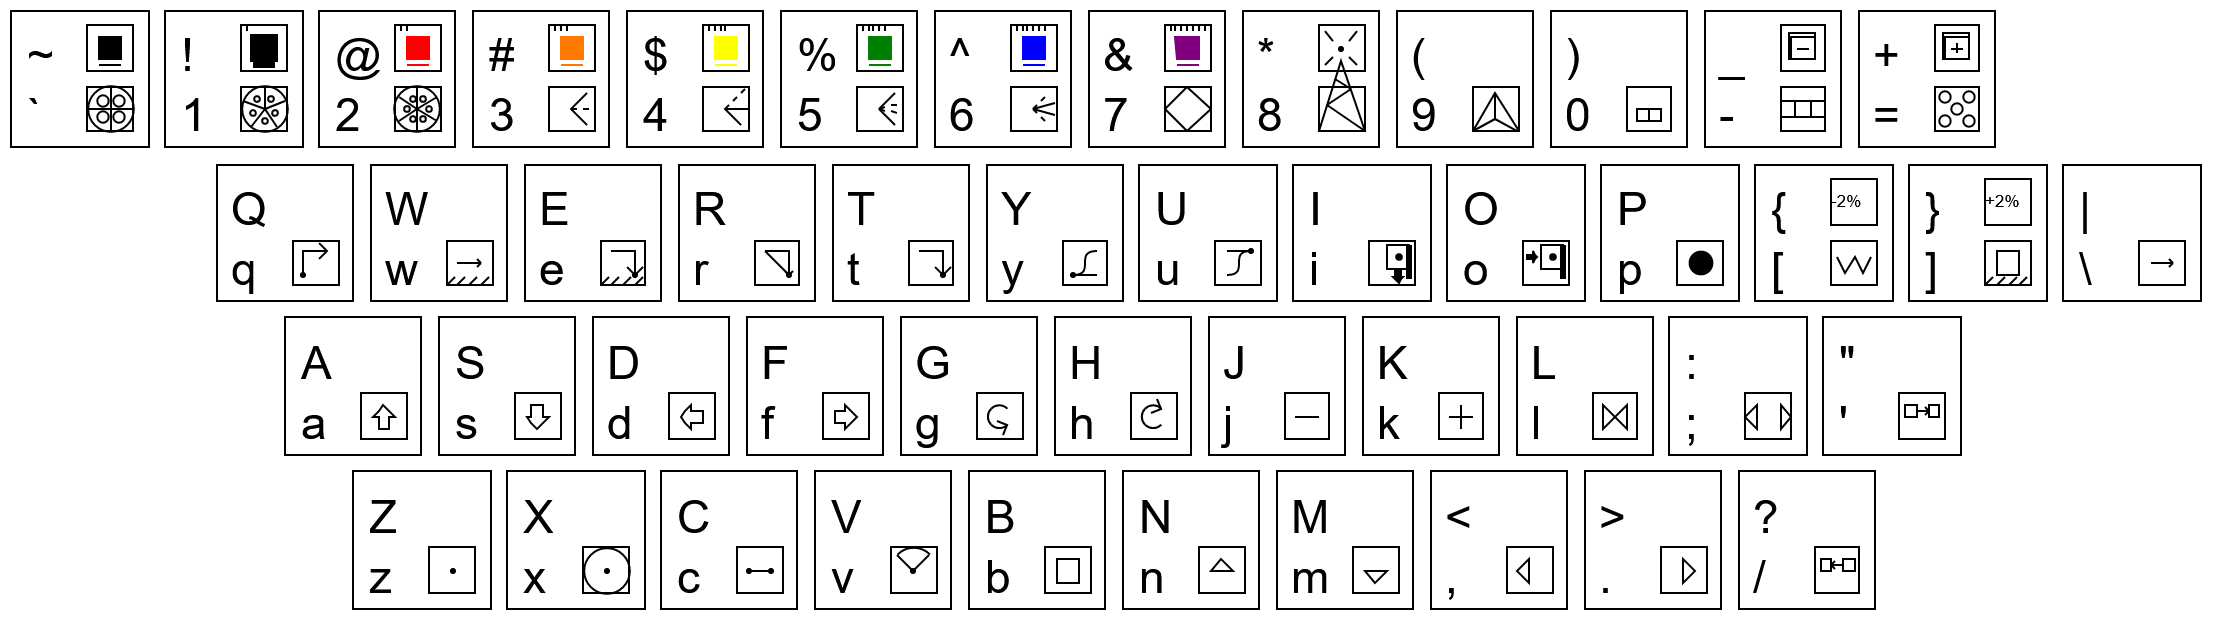
\includegraphics[width=4in]{figures/web2d/keyboard.png}
	\caption[keyboard]
	{Keyboard layout.  Strike a key to add an action to the glyph you are editing.  Arrow keys and backspace allow for editing the whole glyph.  Up and down arrows move to the end or beginning of the glyph.}
\end{figure}

The control panel of soft keys should be pretty self-explanatory: the buttons do the same thing as the keys on the keyboard and are there to make the system work with a touch screen when no physical keyboard is connected, as with smart phones and tablets.

With the ability to edit the main glyph, the best way to learn the language is to just try stuff.  This chapter is largely pictorial.  Go through the figures and try to copy them on the system you are using, play with all the different symmetries, scales, layers, and functions.  To save a symbol, hit the save icon which is in the far left of the menu bar at the top of the screen.  When you have saved a symbol you can see it and download it from the Symbol Feed, which is an icon three in from the left showing equilateral triangles separated by an arrow.  Each symbol is stored as both a bitmap in .png format and a vector graphics file in .svg format.  What is listed in this Feed is simply a sequence of stored files in the directory symbolfeed/, which exists on every Geometron server.  Each file is named with the UNIX timestamp which describes the exact moment it was created.   The Symbol Feed, like all Feeds in the System, also has delete buttons to delete any of the symbols in the Feed, following the Law of Geometron that everything dies.  If you click on an .svg file in the Feed, it will load that symbol into the editor, and you can then go back and edit a copy of it, and save it again to make a modification.  The Symbol Feed also has an upload button just like the Local Image Feed, which lets you upload .svg files from other systems and allow you to edit them using the copy as a template.  Thus we can freely replicate, edit, delete and replicate again.

Move the cursor around, draw circles and lines and squares.  Make polygons, explore scales and symmetries. Try out the Bezier path drawing.  Play with colors.  Make closed and open paths.  When in doubt, destroy it all and start over. 

As you create and edit the main glyph, the address sequence will update live in the text field next to the one where the cursor is for editing.  This will be a sequence of numbers all of which begin with 0.  As with all other parts of the Geometron system, the ability to share information instantly across the world with it is of the highest importance. If you copy the sequence of addresses in that field to the clip board and send it via text message, email or pastebin to someone else with Geometron, they can paste it in that same field and hit return and they will instantly load the same glyph you created, which they can then edit and send back to you modified.  

What you are editing in the system is not just a glyph but a whole JSON structure which is how we can share a whole symbol including style, position, scale, and custom symbolic language tools.  This structure will be described in more detail below, but you can immediately start sharing them by clicking on the icon which says JSON in the Symbol app.  This will bring up a screen which has the JSON data in a text area, and a set of buttons to export, import, save, or reset.  Reset is important because it is possible to corrupt the data beyond recognition and this gets you back to something which will definitely work.  As with all other components of the Geometron system, this is a human readable text format which is designed to be shared both by direct text messaging and by copy and pasting into public pastebins and sharing the pastebin link.



\begin{figure}
	\centering
	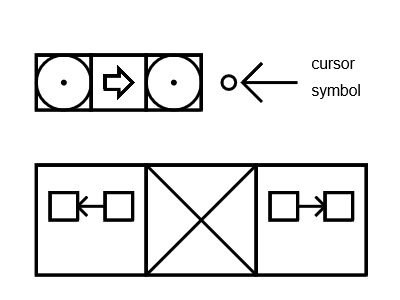
\includegraphics[width=3in]{figures/web2d/cursoredit.png}
	\caption[cursoredit]
	{Edit symbols.  This shows the symbols for moving the cursor back and forward, deleting an action, and also shows what the cursor looks like in a glyph being edited.}
\end{figure}


\begin{figure}
	\centering
	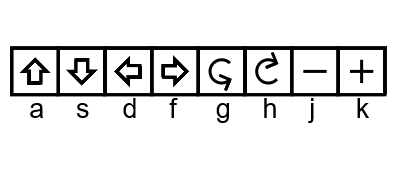
\includegraphics[width=4in]{figures/web2d/move.png}
	\caption[move]
	{Movements.  Arrows move along directions of the lines in the cursor.  Rotation is by the unit indicated by the cursor wing angles. Scale actions are by the current scale value as shown by the dot positions on the cursor.  Letters shown indicate the keys which map to these actions on a QWERTY keyboard with the default settings.}
\end{figure}

\begin{figure}
	\centering
	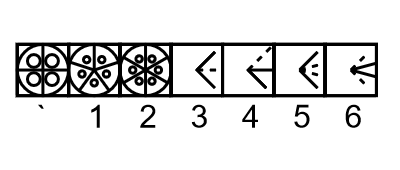
\includegraphics[width=4in]{figures/web2d/angles.png}
	\caption[angles]
	{Angles described by symmetry glyphs.  This also shows the actions to bisect, double, trisect and triple angles, and what keys are used to activate each geometric action.}
\end{figure}

\begin{figure}
	\centering
	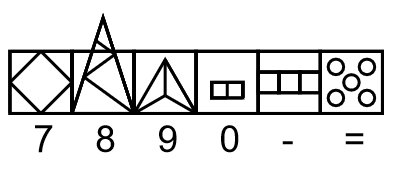
\includegraphics[width=4in]{figures/web2d/scaleactions.png}
	\caption[scaleactions]
	{Scales, along with keys used to map to them in default configuration. There is no relation between the numbers on the keys and the mathematics of the scales.  The scales shown are, from left to right, the square root of 2, the Golden Ratio, the square root of 3, 2, 3, and 5.}
\end{figure}

\begin{figure}
	\centering
	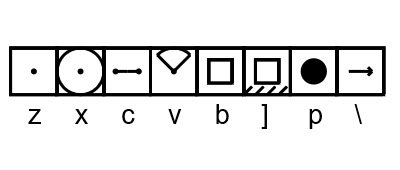
\includegraphics[width=4in]{figures/web2d/basicdraw.png}
	\caption[basicdraw]
	{Basic drawing actions, along with keys used in default configuration to activate them.  From left to right the actions are: draw dot, draw circle of unit radius, draw line segment of unit length, draw arc between cursor wings, draw a square, draw a filled square, draw a filled circle, and draw a line segment while moving forward one unit.}
\end{figure}

\begin{figure}
	\centering
	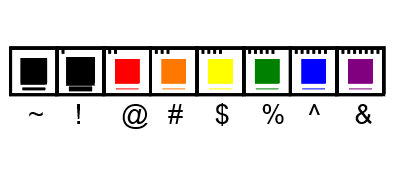
\includegraphics[width=4in]{figures/web2d/colors.png}
	\caption[colors]
	{Layers. Each layer has a line color, line width, and fill color, all of which are set with the Style object using the Style editor app.}
\end{figure}


\begin{figure}
	\centering
	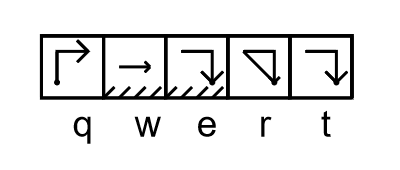
\includegraphics[width=4in]{figures/web2d/pathactions.png}
	\caption[pathactions]
	{Path actions, with keys used to activate them in default state.  From left to right, actions are: start path, draw line segment in path, close a filled path, close an unfilled path, and terminate a path without closing it.}
\end{figure}

\begin{figure}
	\centering
	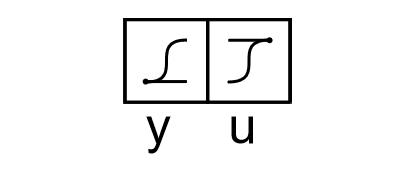
\includegraphics[width=4in]{figures/web2d/bezieractions.png}
	\caption[bezieractions]
	{Start a Bezier Path and terminate it with the y and u keys.}
\end{figure}


\begin{figure}
	\centering
	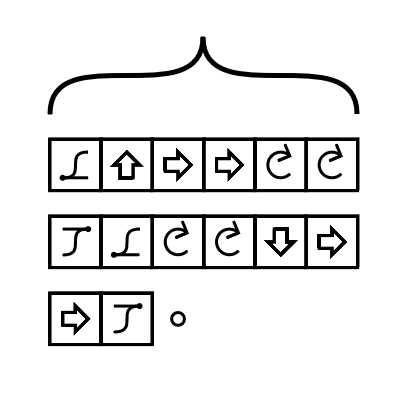
\includegraphics[width=4in]{figures/web2d/bezierbracket.png}
	\caption[bezierbracket]
	{Demonstrating the power of Geometron to make useful symbols with Bezier paths quickly and easily: a twiddle bracket.}
\end{figure}


\begin{figure}
	\centering
	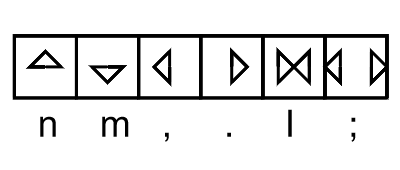
\includegraphics[width=4in]{figures/web2d/panzoom.png}
	\caption[panzoom]
	{Pan and zoom the field of view.}
\end{figure}

\begin{figure}
	\centering
	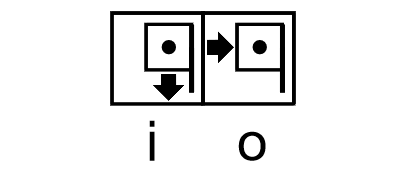
\includegraphics[width=4in]{figures/web2d/flagactions.png}
	\caption[flagactions]
	{Drop a flag, return to flag.  This saves and then recalls the state of the GVM.}
\end{figure}


\begin{figure}
	\centering
	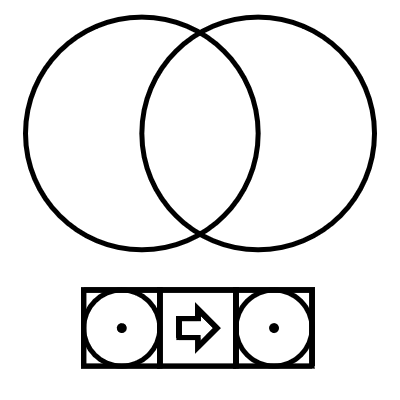
\includegraphics[width=4in]{figures/web2d/vesicapiscis.png}
	\caption[vesicapiscis]
	{The ``hello world'' of geometric programming, the Vesica Piscis.}
\end{figure}
\begin{figure}
	\centering
	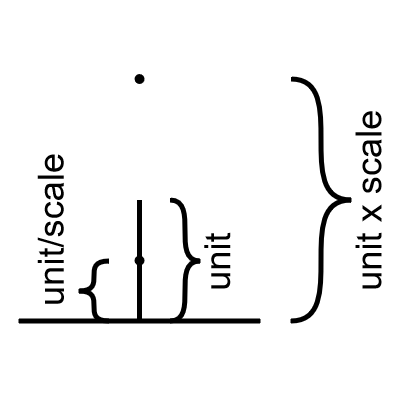
\includegraphics[width=4in]{figures/web2d/cursorscale1.png}
	\caption[cursorscale]
	{Cursor scale.  This shows how scale works with the Geometron cursor.}
\end{figure}
\begin{figure}
	\centering
	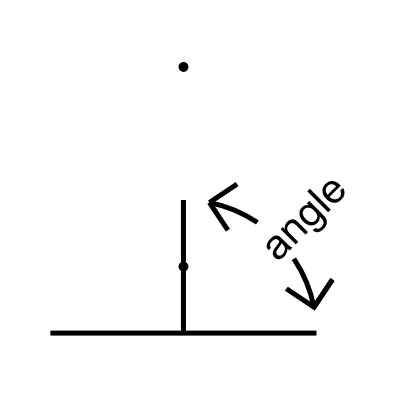
\includegraphics[width=4in]{figures/web2d/cursorangle1.png}
	\caption[cursorangle]
	{Cursor angle. This shows how angles work with the Geometron cursor.}
\end{figure}
\begin{figure}
	\centering
	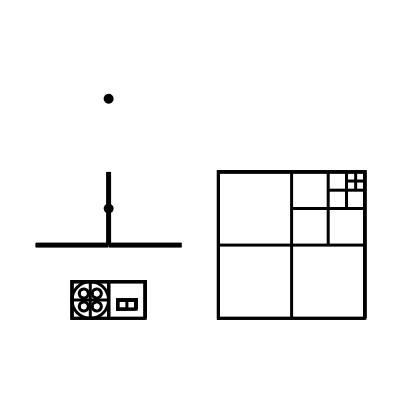
\includegraphics[width=4in]{figures/web2d/cursorsquare.png}
	\caption[cursorsquare]
	{What the cursor looks like with factor of two scaling and a 90 degree angle.  Also shown is a square used in Action Geometry.  Try making the square!}
\end{figure}
\begin{figure}
	\centering
	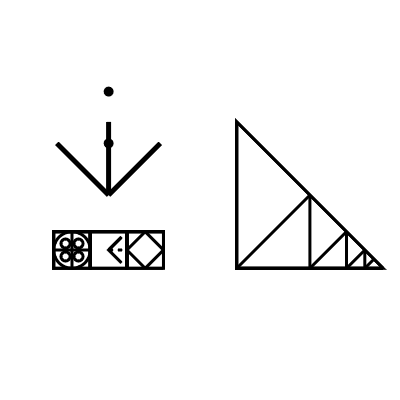
\includegraphics[width=4in]{figures/web2d/cursorroot2.png}
	\caption[cursorroot2]
	{Another example of a commonly used Geometron cursor state, which combines the square root of two with 45 degree angles.  Also shown is yet another shape used in Action Geometry which is also a good exercise to try to copy yourself.}
\end{figure}
\begin{figure}
	\centering
	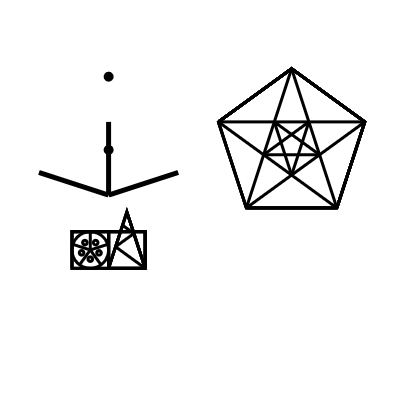
\includegraphics[width=4in]{figures/web2d/cursorgolden.png}
	\caption[cursorgolden]
	{Cursor with Golden Ratio scaling and 72 degree angle for fivefold symmetry work.  Shown is another shape that is helpful to learn to copy, the pentagon/pentagram fractal.}
\end{figure}
\begin{figure}
	\centering
	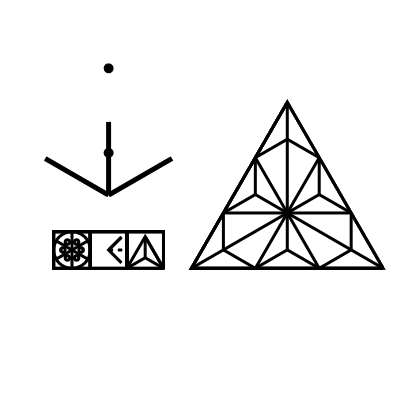
\includegraphics[width=4in]{figures/web2d/cursorroot3.png}
	\caption[cursorroot3]
	{Cursor with square root of three scaling and 60 degree angle.  This can be used to make the kinds of symbols shown, and replicating that is a useful exercise, as well as working through the deconstruction of the six pointed star and hexagon.}
\end{figure}
\begin{figure}
	\centering
	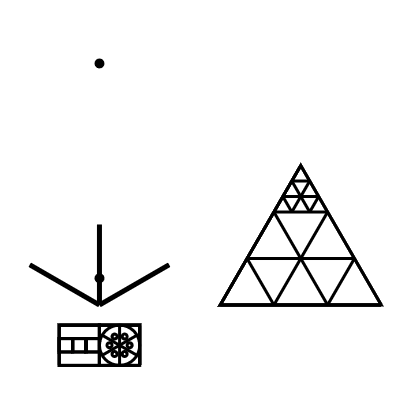
\includegraphics[width=4in]{figures/web2d/cursor3.png}
	\caption[cursor3]
	{The cursor with a 60 degree angle and factor of 3 scaling, along with another exercise to copy.}
\end{figure}
\begin{figure}
	\centering
	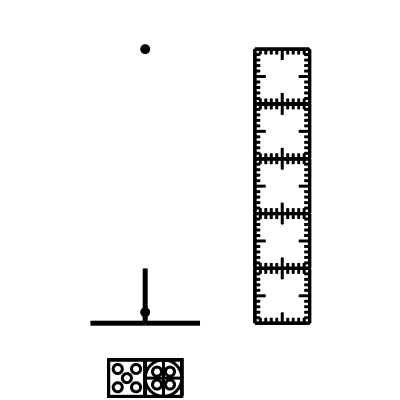
\includegraphics[width=4in]{figures/web2d/cursor5.png}
	\caption[cursor5]
	{Cursor with scaling factor 5 and right angles. This can be used along with scale factor 2 to make things with scale factor 10.  What is shown to copy as an exercise is a ruler constructed using this tool which can be made physical using a laser cutter as discussed in the Action Geometry chapter.}
\end{figure}


Each instance of the Geometron Virtual Machine has a style object, which defines 8 layers, numbered from 0 to 7.  Each style has a line color, line width, and fill color.  The properties of the style object are stored in the JSON file data/currentjson.txt which is used by the app symbol.html to edit graphics which are used by the rest of the Geometron system.  

\begin{figure}
	\centering
	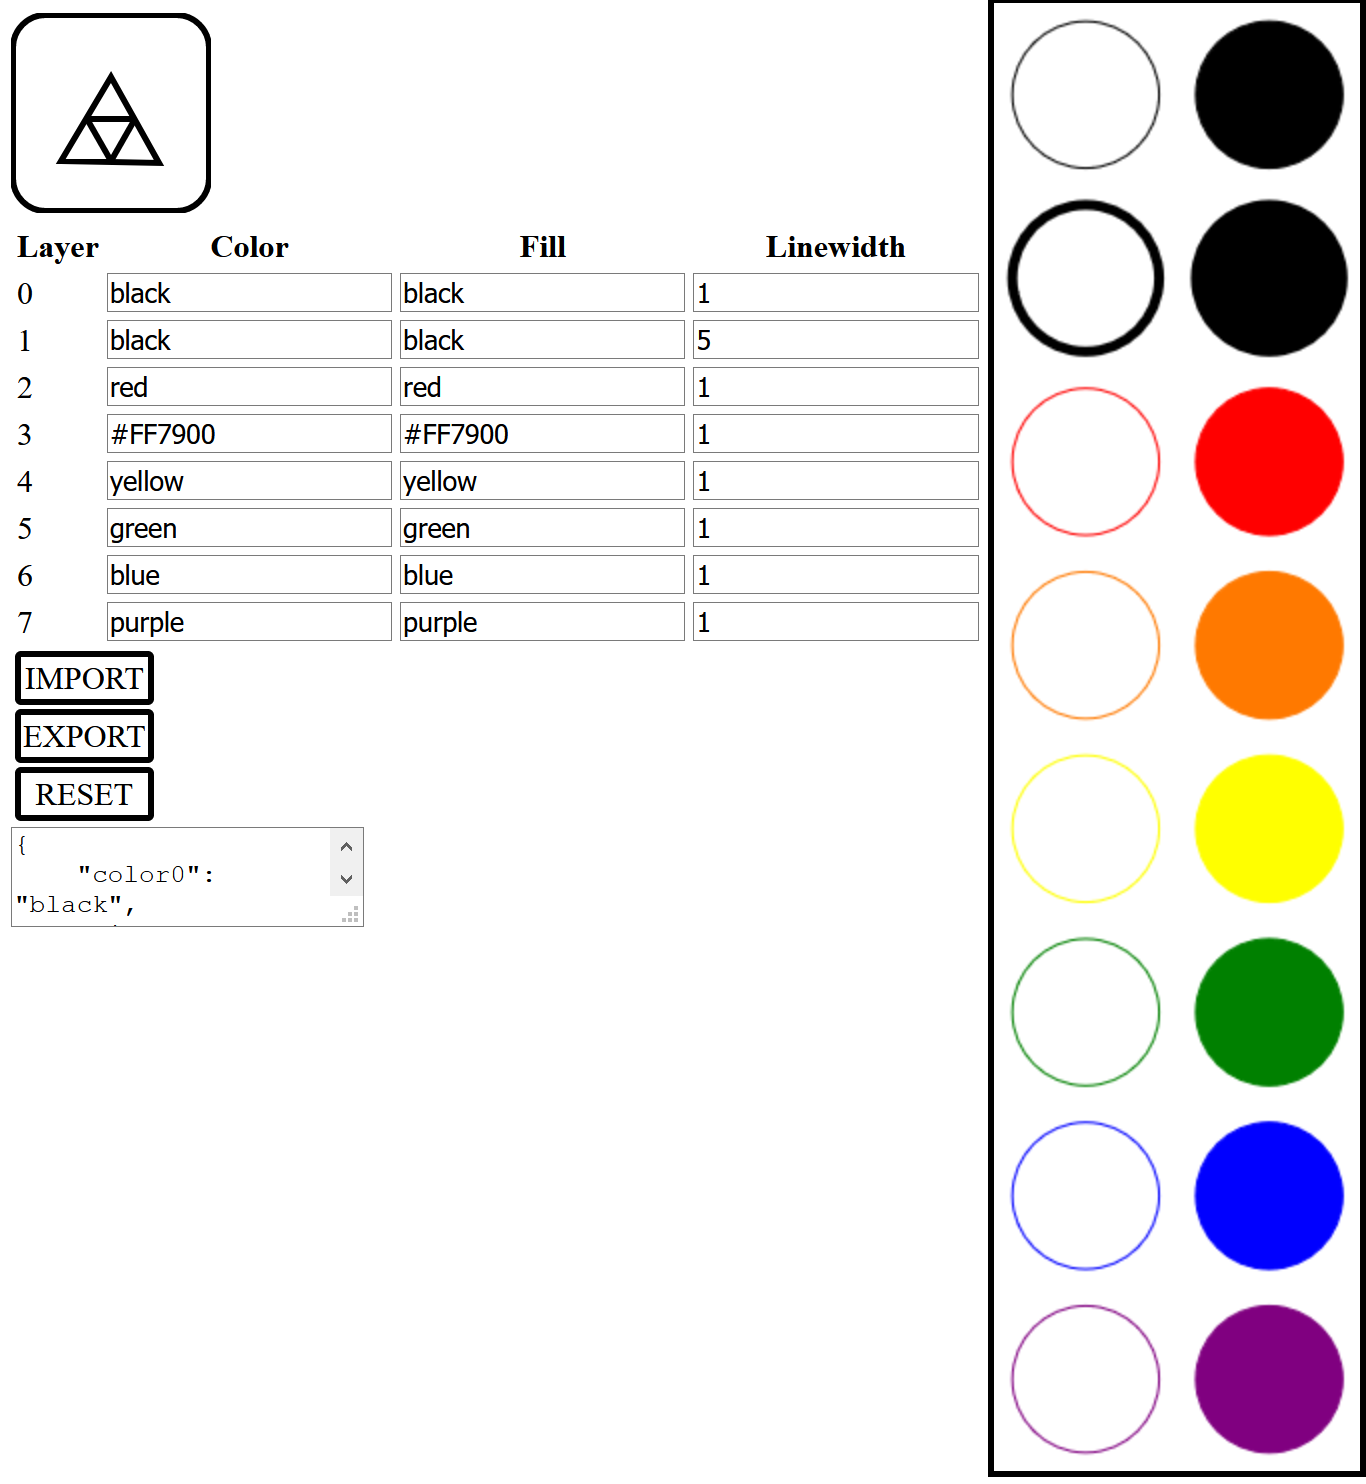
\includegraphics[width=4in]{figures/web2d/styleeditor.png}
	\caption[styleeditor]
	{Screen shot of the style editor app at styleeditor.html.  The display on the right hand side of the screen shows an unfilled circle and filled circle of each layer's style.  The text area in the bottom left of the screen is used to import and export style data, which can be saved offline and shared with other users via text message, email, etc.  The RESET button resets the style to a standard setting, which will erase any changes made to the existing style. Enter new values into any field to immediately change it.}
\end{figure}

While the style app edits the data file currentjson.txt which applies to the whole Geometron object used for symbol editing, the importing and exporting of data for sharing with other users only includes style information, without the rest of the JSON data.  This allows styles to be separated from the rest of the information for the purposes as usual of building a robust remix culture where Geometron users can constantly be sharing each piece of the system.  The EXPORT button will always post the current style JSON in the window in the lower left of the screen.  IMPORT will import the data, and RESET returns it to a default state.  Try creating your own new style with unusual line widths and colors, then exporting it and saving it offline, sharing it with other users, etc.  

Colors are in the format of HTML/CSS/JavaScript, and can be either names of colors like ``red'' or RGB color values like ``\#00ff00''.  This last format is a number in base 16 which has three 2 digit numbers in it(numbers between 0 and 0xFF), where the three numbers are values of red, green, and then blue.  So black is \#000000 and white is \#FFFFFF.  Any value where all three numbers are the same, like \#808080 will be a shade of grey.   Colors can be partially transparent by adding a fourth hexidecimal number which represents opacity.  So fully opaque red is \#FF0000FF, and red with half transparency is \#FF000080(80 because 8 is half of 16, this is actually 128 in decimal).

The next section of the JSON we want to know how to edit in order to be able to make useful graphics is the setup, edited in the app setup.html.  Setup edits five numbers, all of which are in units of pixels: x0, y0, unit, width and height.  Width and height are the width and height of the graphics file currently being edited or created.  When a Geometron glyph is drawn with a given GVM, it starts with x and y equal to x0 and y0. Setting these two values is therefore effectively setting the horizontal and vertical offset of the field of view of the symbol.  When we activate a pan function within the symbol.html app what we are really doing is modifying the values of x0 and y0 in the JSON file.  These are done manually in this app.  Finally, unit describes the initial unit value of the GVM.  This is essentially the scale factor.  So again when we activate the zoom functions in any other symbol editor what we are really doing is making changes to the variable unit in the global JSON file.    

The app setup.html has five fields in which to enter the numbers for the five values. There is also a reset button to restore default, with a 600 by 600 pixel square and 80 pixel unit centered in the center.  

The final section of the global JSON file which defines the settings of the symbol app is the shape stack.  This is a subset of the hypercube, and is stored both in the JSON file data/hypercube.txt and also data/currentjson.txt.  When vector graphics files are saved, this shape stack is stored inside them so that they can be reloaded with the whole stack.  The creating and sharing of useful shape stacks will be discussed in the next chapter.  This is a very important element of the system as it allows for the rapid dissemination of specialized graphical languages for things like drawing circuit diagrams or subway maps.

Other links to other apps from the main symbol app are to the keyboard editor, which edits the layout of the keyboard, the Hypercube editor, which edits the entire Geometron Hypercube, and the Font editor, which edits just the font.  All these have the capacity to share human readable text from system to system as is the case with everything in the Geometron system.  The font and Hypercube apps are still somewhat crude and could be improved substantially, but they do work for their intended purpose with a little bit of fiddling.  They will be used through the rest of this work as we delve into more applications of Geometron geometric programming. 

There is also an app separate from the main symbol editor called symboltrace.html, which allows you to trace images into symbols, which you can then copy and paste at will.  This takes images from both the local and global image feed, so you will need to load the image you want to copy in one of those first.  Still another random app of some utility is action2symbol.html, which converts a glyph made up of actions to one made up of the symbols which correspond to those actions.  This is how we put glyph symbol spelling into a symbol, which is very useful for documenting things which reference the language and how it is used.  

Part of the power of the Symbols in Geometron is how they are integrated into the rest of the system.  When you save a symbol, a copy of the base 64 encoded bitmap is stored in the textfeed which gets used by the Map editor to create maps.  This means that you can create a symbol, then go import it into the Map editor immediately.  Because it is a self-contained image url which has the actual graphics encoded in the url rather than as an external file, this Map you create can then be shared with anyone else anywhere in the world with another Geometron system and they will be able to import and use that Map without any other image files.  This ability to instantly integrate Symbols into Maps can enable a sort of graphical meme system which can be extremely powerful for numerous applications.


Also, we note that all icons used in the Geometron system are created using the Symbol editor described in this section.  These are then stored in the directory iconsymbols/.  This directory is all copied with every copy of the whole self-replicating system.  Therefore if you want to add another symbol to the next copy of the system, just add your new symbol to this directory, run dnagenerator.php, and the next instance will have your new image.

If you are a coder, you can read the whole of the system documented in this chapter in the JavaScript library stored at jscode/geometron.js, which is on every instance of the system.  You can of course edit this, and your edits will replicate along to the next instance of the system.


\begin{figure}
	\centering
	
\includegraphics[width=3in]{figures/shapes/blank.png}
\end{figure}
\begin{figure}
	\centering
	
\includegraphics[width=3in]{figures/shapes/blank.png}
\end{figure}
\begin{figure}
	\centering
	
\includegraphics[width=3in]{figures/shapes/blank.png}
\end{figure}

\chapter{Shapes and Fonts}
\section{shapes and fonts: examples}

\begin{figure}
	\centering
	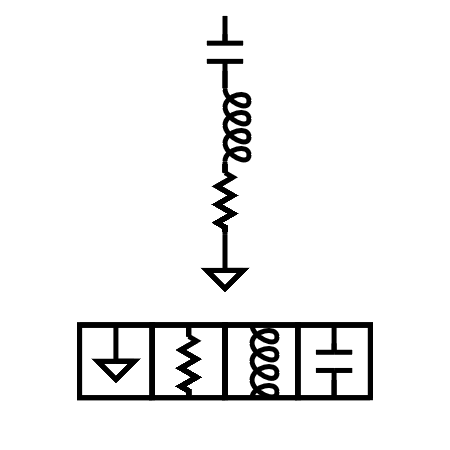
\includegraphics[width=4in]{figures/rlc.png}
	\caption[RLC]
	{RLC circuit.}
\end{figure}

\begin{figure}
	\centering
	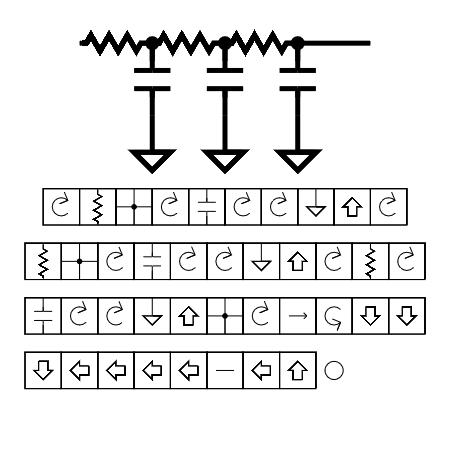
\includegraphics[width=4in]{figures/rcline.png}
	\caption[RCline]
	{RC line circuit.}
\end{figure}


\begin{figure}
	\centering
	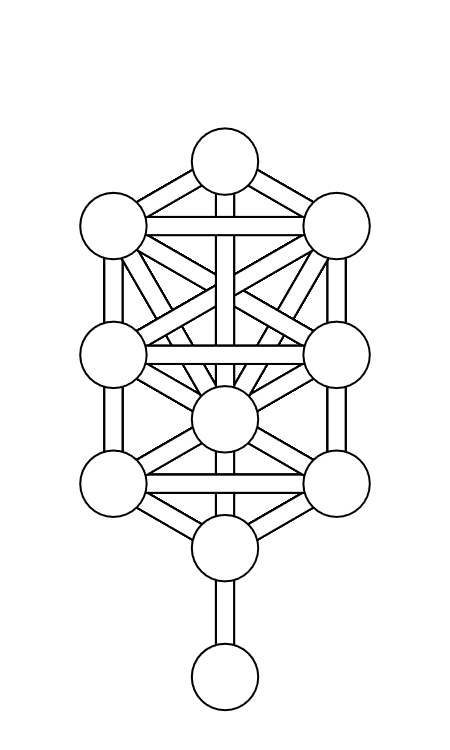
\includegraphics[width=4in]{figures/treeoflife.png}
	\caption[treeoflife]
	{The Tree of Life from Jewish mysticism.}
\end{figure}

\begin{figure}
	\centering
	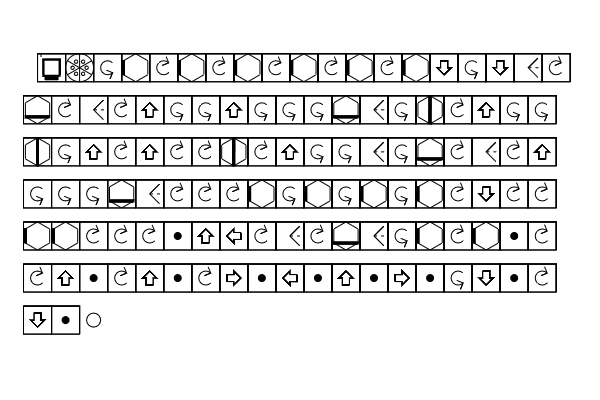
\includegraphics[width=4in]{figures/treeoflifespelling.png}
	\caption[treeoflifespelling]
	{Symbol glyph spelling of Tree of Life. What makes things like this easy to make is building up building blocks like the cross pieces of all different scales, and the use of universal symmetries and scales(6 fold, 12 fold, and the square root of 3 and 2).}
\end{figure}




\begin{itemize}
\tightlist
\item
editing shape stack, workflow, how to share, upload, download, send and store, same with fonts, connect to hypercube
\item
basic shapes built into 0200 thru 0217, how it's all connected to 01xxx
\item
pixel fonts
\item
laser cut fonts
\item
signal flag font
\item
general circuits
\item
quantum circuits
\item
graph theory, with digression into how to operate Maps with mathjax formatting for fully tex compatible graph theory figure creation
\item
quantum logic gates
\item 
classical logic gates
\item
standardized icon design for geometron system
\item
katakana
\item
hebrew
\item
laser cut shape set shape stack
\item
laser cut ruler
\item
laser cut protractor
\item
tree of life from western occult practice
\item
penrose tiles, fun with golden ratio, fivefold symmetry
\item
cross stitch design
\end{itemize}
\chapter{Action Geometry}
We create a geometry in which constructions are whatever methods are most effective for replicating objects from trash and natural materials.  In classical geometry many of us learned in school, we are restricted to the use of the compass and straight edge.  Then in the geometry used in computers, everything is reduced to numbers and geometry becomes arithmetic.  But in Action Geoemtry we use the technology available today to make shapes which carry information about the symmetries and scales we will use for common constructions.  

Unlike in school where we learn to construct things at random, in Action Geometry the purpose of all geometric construction is to replicate things made out of trash in the way most beneficial to the people in our community.  So to choose geometric tools we look at what is available and what we can build, and then build up our geometry around that.  

The materials we start out using are cardboard, scrap cloth, bamboo, and high density polyethylene from milk bottles.  We also use some commercial off the shelf parts and tools, as well as all the tools of Geometron.  The Geometron language documented in the earlier chapters can be used to make geometric shapes which can be sent to a laser cutter.  The shapes can also be traced off of a screen with thin paper and a pencil, the paper cut out and laminated, and then used as a physical construction.  Or if you have a paper printer, you can print the file you create with Geometron.   The shape set is shown in one of the figures.   It includes a collection of shapes that all use 3 inches as a reference, and which contain information about the standard symmetries and scales from geometron.  This includes 90 degree, 45 degree, 72 and 36 and 108 degree, 60 and 30 degrees, and the Golden Ratio, square root of two, and square root of three.  Along with a standard Geometron ruler 6 inches in length, this set of shapes forms the basis of our whole construction method. 

These shapes can be used to construct a wide range of shapes very quickly which can replicate, using the plastic parts to create a template from cardboard, which gets cut out and then used to trace out the same pattern again and again.   This is self-replicating geoemetry!  You can imagine a design, lay it out using standard symmetry and scales on any Geometron server, then use that design as a guide to hand construct that same shape once in cardboard, cut it out and copy it.  Also, you can take the text data for the symbol you created on the Geometron server, put that in a public pastebin and share that with another person.  That person can copy the data into their local Geometron server, edit the layout, and then use their copy of the shape set to make their copy of the cardboard template, then use a sharpie and box cutter to replicate again and again.  Note also that this replication is cascading, like a critical nuclear reaction: each copied piece of cardboard is itself a template which can be used to trace out to cut out another copy in more fresh cardboard.  So the Mathematics of this if there is a large swarm of people going into a very large feed of corrugated cardboard is that there can be exponential growth of the number of copies of a cardboard shape for a certain number of generations.  This shows how scaling in a self-replicating economy can do things that are not possible in a consumption/production economy.

We use the simplest possible constructions to achieve any given task.  The first things we build are the ArtBox, which is a self-replicating box of art supplies. The figures show the layout of how you can use just a 6 inch equilateral triangle repeated 10 times in the right layout to make an attractive art purse.  The skin is wrapped in colored duct tape applied from the Tape Snake, also described in the figures.  The box contains the shape set and ruler of Geometron described above and in the figures, box cutters, sharpie markers, scissors, googly eyes, and more clothesline.  With this set of art supplies, all you need is this ArtBox fully loaded with the Tape Snake, and you can transform a feed of corrugated cardboard trash into an output feed of the same box which is then used to make more boxes and so on.  

Note that this ArtBox is made from a combination of the octahedron and tetrahedron.  Using these two is a tool we can repeat again and again for simple design of useful structures with the minimum of complexity to replicate.  Each of these also contains the open brand of Trash Robot, which is rainbow and googly eyes.  Each box has googley eyes and a black duct tape mouth to make a face.  This is a recognizable brand identity, but it belongs to no one.  It is not property.  So it can replicate freely.

Another basic construction from cardboard is the Golden Pyramid, which is shown in two of the Figures.  This can be used as the enclosure for a very wide range of technologies, from battery packs to Raspberry Pi Geometron Servers, to lights, robot controls, or stereo equipment.  It has a 6 inch square base, a 3 inch square top, and each side has the same angles as for the Golden Triangle(72 degrees).

Textile arts are created by finding black cloth from scraps and plain black clothes and sewing on geometric patterns with bright solid rainbow colors of felt or some similar material.  Text are created by starting with a square and removing as little material as possible in as simple as possible layout to depict a letter.  The Geometron Raspberry Pi servers are carried around in black cloth bags with a Raspberry Pi Penrose tile layout as shown in one of the figures and a 6 foot clothesline Trash Tie drawstring.  There are two types of Trash Tie: the six foot clothesline terminated in duct taped ends, and the 18 inch nylon parachute cord section with burned ends.  Small black cloth bags are sewn with small trash ties as draw strings, and these have symbols sewn on them representing the different types of clay icon token described in a later chapter.  Large bags are also used to carry around the printer which makes the clay tokens which go in the bags.  Some figures of the textile are left blank, these are filled in by hand in the illuminated manuscript in physical copies, and shared in person along with the physical textile arts and crafts.


Skeletron is a method of building structures of all kinds for supporting technology as well as building shelters and light industrial infrastructure.  The Trash Pole is a roughly 6 foot long piece of bamboo with quarter inch holes drilled just in from each end as well as in the center of the pole, all wrapped in rainbow colored duct tape from end to end.  These poles can be joined at the ends by tying the smaller Trash Tie(18 inch nylon parachute cord) through the holes and tying a square knot.  With ends joined, we can construct again a wide range of three dimensional geometric structures using basic geometry of tetrahedra, octahedra, and small deviations from those.  These constructions can then be sketched out by hand or via Geometron and shared freely across the Street Network, again forming self-replicating physical geometric construction.  These poles can be used to build useful things, which induces passerby to donate duct tape and go scrounge for more bamboo, and join in the work of assembly, making a swarm just expand potentially very fast, as long as the rate of new contributors is maintained.  This again stresses the importance of building a powerful open brand.  If the extreme rainbowcore aesthetic can be used to get peoples attention, that will make something which spreads in an organic way.  Not viral, as it is not just information in a fixed system, but organically, as a physical thing is being replicated.  The bamboo could be substituted with any other straight object, like broomsticks, fenceposts, harder solid sticks, etc.  This whole scheme can of course also be scaled up and down with any other scale and material of straight thin structural element.  

This type of triangular replicated structure can be very strong and can build up fractal trusses to make huge complex structures both on land and in and on water.  Skeletron forms the basis of a totally decentralized modular construction method.  The sticks can form frames, and to build shelters from rain and wind, plastic bottles can be cut into strips and those stripes woven and laminated into giant plastic sheets which can be affixed to the frames.  This can be combined with cardboard and paper trash and things like polystyrene trash to insulate the structure, to make robust livable shelters which can scale based on our Action Geometry.  To become an artist in this form of construction, you will want to study deeply and practice extensively with all constructions involving tetrahedrons and octahedrons.  Experiment, study, document, share, replicate.  

Because we have a lot of things designed to be hung from Trash Poles using Trash Ties, we also want modular hooks to suspend things from the Trash Poles.  These are the S-Hooks, which are made from a stack of 4 corrugated cardboard cutouts wrapped in rainbow duct tape, with googly eyes for branding.  The construction for this is done using the 3 inch square shape from the basic Action Geometry shape set, and is shown in the figure.  Again, each time an S is cloned, that clone is the template to make more S's, so this part can replicate with an exponential growth if it is fed into the right trash feed with the right group of people in a local Trash Robot swarm.

This chapter describes then a set of objects which we can share in a physical place by a physical Geometron Server.  These can be shared, used, given away, bartered, sold, improved upon, and sent along to other places in the world to seed new swarms.  A Geometron Trash Camp might include any subset of the things described here.  Huge camps might have a whole village of livable shelters made from Skeletron with Trash Sheet, insulation, HVAC systems, power, industrial production machinery, telecom infrastructure, water purification, sanitation, and agriculture, and span a substantial area.  A small camp might just be a Server on a Golden Pyramid, hanging from a dumpster at a truck stop via a Trash Tie, delivering documents over a hotspot on a smart phone.  But whatever tools and materials we use, we can rely on the power of the Geometron geometric language to replicate constructions from community to community via the Street Network so that we can reach all of Humanity who wants to share.

\begin{figure}
	\centering
	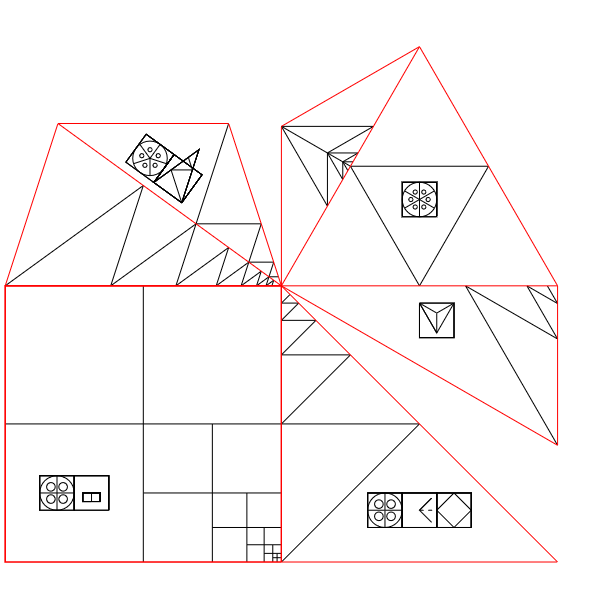
\includegraphics[width=3in]{figures/actiongeometry/shapeset.png}
	\caption[shapeset]
	{Shape Set. This is the basic shape set of Action Geometry.  It has the symmetries and scales of Geometron. What is shown should be printed exactly 6 inches wide, making each shape three inches on a side.}
\end{figure}

\begin{figure}
	\centering
	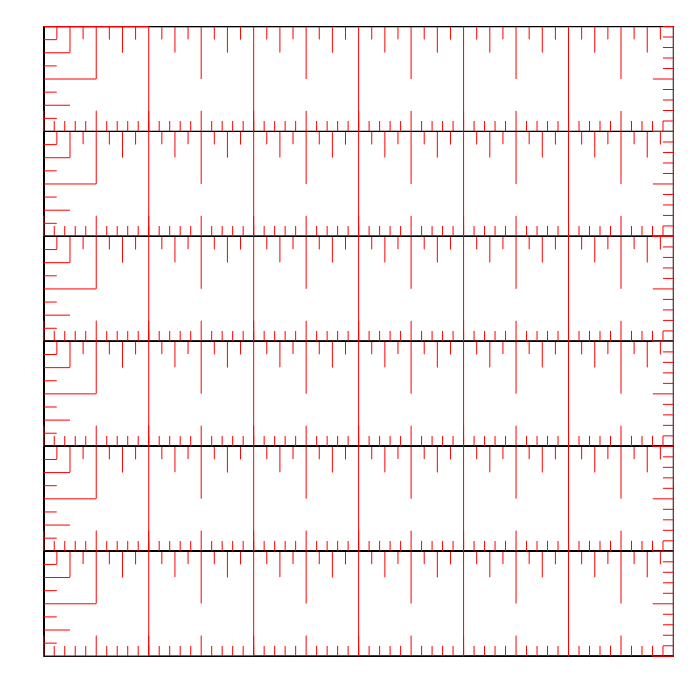
\includegraphics[width=3in]{figures/actiongeometry/rulers.png}
	\caption[rulers]
	{Rulers.  Make this 6 inches wide and each ruler is a 6 inch ruler, 1 inch across, with both tenth and factor of two divisions.}
\end{figure}

\begin{figure}
	\centering
	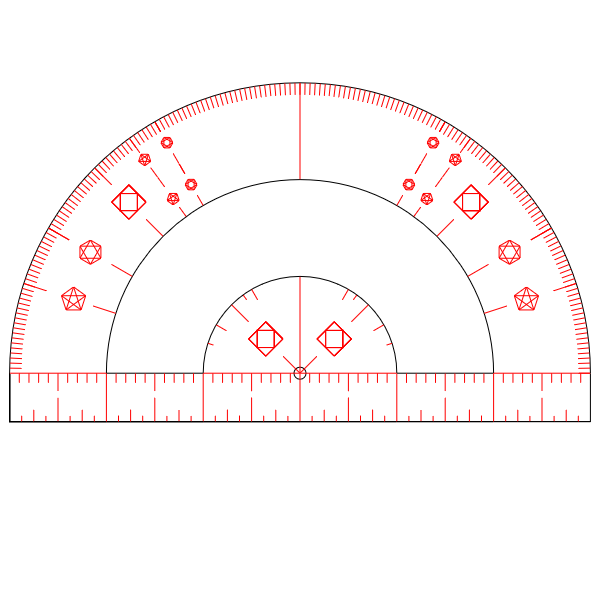
\includegraphics[width=3in]{figures/actiongeometry/protractor.png}
	\caption[protractor]
	{Geometron protractor.  While not really needed for Action Geometry, this protractor is a nice accessory which emphasizes Geometron symmetries rather than numbers, and allows drawing of circles of radius 3,2 and 1 inch without a compass.  This is mostly useful if cut out with a laser cutter.}
\end{figure}


\begin{figure}
	\centering
	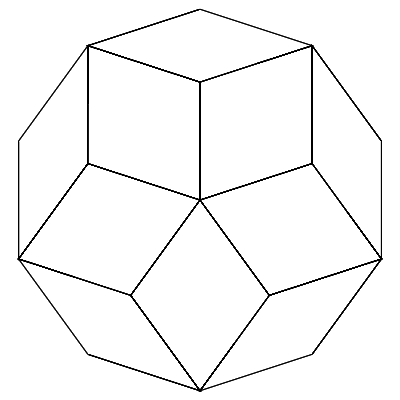
\includegraphics[width=3in]{figures/actiongeometry/penrose.png}
	\caption[penrose]
	{Penrose. Penrose tiles, the rhombi construction.  Copy, print, trace, or laser cut these, and use them to make logos, icons and symbols with some kind of meaning which other people can easily replicate.  The Shape Stack can by copied from someone which has these two shapes, and that can be used to create designs on Servers, which can then also be shared with your community who can all copy your highly recognizable design which has the Trash Robot metabrand as well as whatever symbol you have created or edited.}
\end{figure}

\begin{figure}
	\centering
	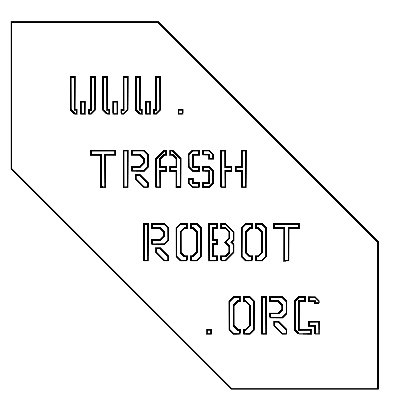
\includegraphics[width=3in]{figures/actiongeometry/stencil.png}
	\caption[stencil]
	{Spray paint stencil for laser cutting. You can use the Geometron software, selecting the built in laser font, to make a custom spray paint stencil pointing to the domain name which points to your Geometron server.  If you are Trash Robot, that can be Trash Robot, but we mostly point to a local non-property place.}
\end{figure}


\begin{figure}
	\centering
	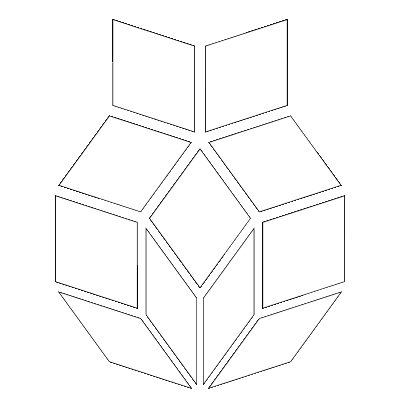
\includegraphics[width=3in]{figures/actiongeometry/pilogo.png}
	\caption[pilogo]
	{Construction of the Raspberry Pi logo for server bags. The top two shapes are green the rest are red.}
\end{figure}


\begin{figure}
	\centering
	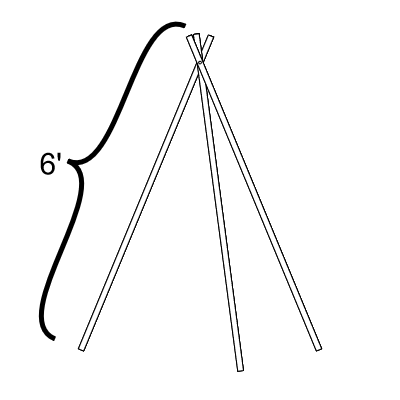
\includegraphics[width=3in]{figures/actiongeometry/skeletrontripod.png}
	\caption[skeletrontripod]
	{Skeletron tripod.  Three 6 foot bamboo trash poles wrapped in rainbow colored duct tape with quarter inch holes drilled just back from the end.  An 18 inch nylon parachute cord trash tie is used with a square knot to secure the top.  Many things can be hung from this, including servers, terminals, robots, boxes, flags, lights, textile arts and pendants on more trash ties.  The tripod can be carried over the shoulder to be mobile, without untying the joint at the top for rapid deployment.}
\end{figure}

\begin{figure}
	\centering
	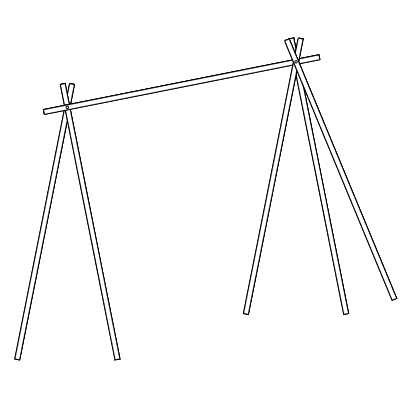
\includegraphics[width=3in]{figures/actiongeometry/skeletron2.png}
	\caption[skeletron2]
	{Skeletron cross bar configuration.  Two tripods can be converted into this stable configuration quickly to have a horizontal cross bar which S-Hooks can hang from to hang numerous objects of all kinds.}
\end{figure}


\begin{figure}
	\centering
	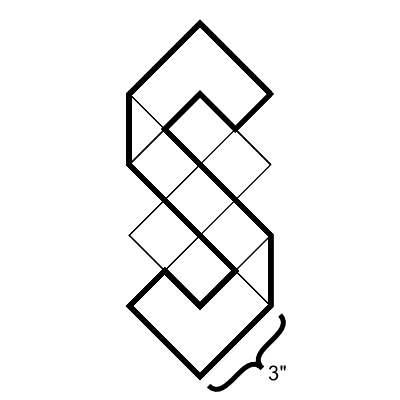
\includegraphics[width=3in]{figures/actiongeometry/shook.png}
	\caption[shook]
	{S-Hook.  Note the repeated use of the square shape, and the use of the 45 degree triangle, making this easy to replicate using the Shape Set.  This hook is used to hang things from the Trash Poles in Skeletron. Fabricate by stacking 4 identical layers of corrugated cardboard cut in this pattern and wrapping them in rainbow colored duct tape.  Googly eyes can then be applied.}
\end{figure}


\begin{figure}
	\centering
	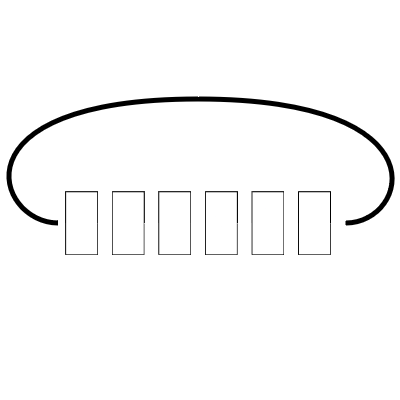
\includegraphics[width=3in]{figures/actiongeometry/tapesnake.png}
	\caption[tapesnake]
	{Tape Snake.  Duct tape rolls of all useful colors, namely the rainbow colors plus black and pink, are strung on a 6 foot Trash Tie made from a clothesline which is looped through twice and secured with a square knot in a bight(like a bow on a tied shoe) for rapid replacement of rolls as they are used.}
\end{figure}


\begin{figure}
	\centering
	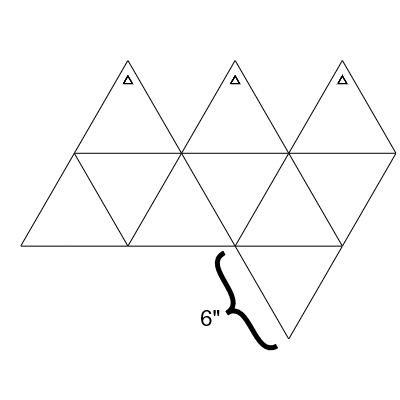
\includegraphics[width=3in]{figures/actiongeometry/artboxnet.png}
	\caption[artboxnet]
	{ArtBox Net.  Cut out 10 equilateral triangles from corrugated cardboard.  Duct tape the joints as shown.}
\end{figure}

\begin{figure}
	\centering
	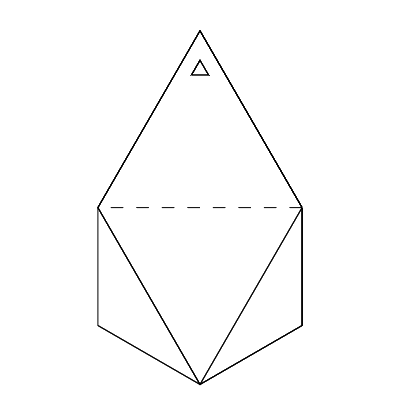
\includegraphics[width=3in]{figures/actiongeometry/artbox.png}
	\caption[artbox]
	{ArtBox assembly.  The fully assembled box is a tetrahedron on an octahedron.  It should contain the means of its own replication, which is a box cutter, a ruler, an equilateral triangle, and a sharpie, along with a Tape Snake for duct tape fabrication, extra Trash Ties, and googly eyes.  Use duct tape colors in sequence to create a fully rainbowed effect, then apply googly eyes and add a black duct tape mouth.}
\end{figure}

\begin{figure}
	\centering
	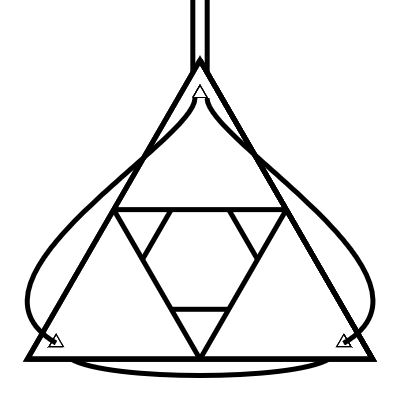
\includegraphics[width=3in]{figures/actiongeometry/artboxtop.png}
	\caption[artboxtop]
	{Top view of ArtBox.  Cut out little triangles in each of the top three petal triangles with the box cutter.  Thread a 6 foot Trash Tie with ends taped with duct tape as shown, and tie off the two bitter ends with a double figure eight knot for convenient purse-strap geometry.}
\end{figure}


\begin{figure}
	\centering
	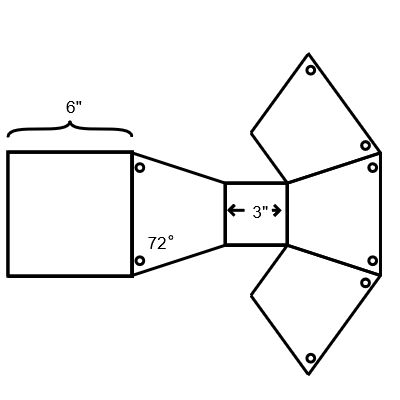
\includegraphics[width=3in]{figures/actiongeometry/pyramidnet.png}
	\caption[pyramidnet]
	{Pyramid net.  Use the Shape Set and Ruler to cut out corrugated cardboard patterns and stitch together with duct tape as shown.  Cutouts include a 6 inch square, a 3 inch square, and four trapezoids with 3 inch top and 6 inch base with 72 degree angles on the bottom angles.}
\end{figure}

\begin{figure}
	\centering
	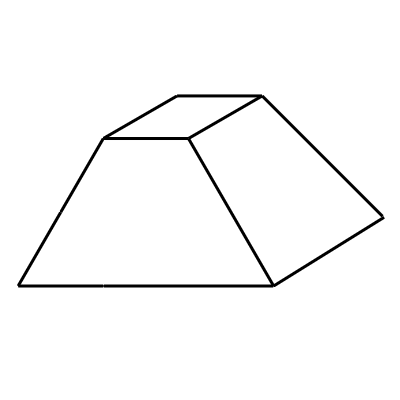
\includegraphics[width=3in]{figures/actiongeometry/pyramid.png}
	\caption[pyramid]
	{Pyramid assembly.  Fold it all up and then cover the whole thing in a skin of rainbow duct tape.  Open the base, insert technology and re-seal.  Add cutouts as needed for cords in and out.}
\end{figure}

\begin{figure}
	\centering
	
\includegraphics[width=3in]{figures/shapes/blank.png}
    \caption[bags]
	{Bags are cut from black cloth, which can be scrap.  Black cloth bags are sewn up with Trash Ties as draw strings.}
\end{figure}


\begin{figure}
	\centering
	
\includegraphics[width=3in]{figures/shapes/blank.png}
    \caption[outfit]
	{Draw your personal Geometron outfit which is black with solid rainbow color felt or similar cloth sewn on in geometric patterns and geometric font.}
\end{figure}
\begin{figure}
	\centering
	\includegraphics[width=3in]{figures/shapes/blank.png}
    \caption[outfit]
	{Draw your Flag.  A Flag is a black square cloth about 3 feet on a side, with a sewn hem with loops to tie a trash tie.  It is decorated with solid block letters and geometric shapes cut from solid color rainbow felt or similar.  All elements can be from scrap.  Flags point to domains in places.} 
\end{figure}

\chapter{Machine Control}
\section{Machine Control}

\subsection{democratization of machines}

We should have as much control as possible of every machine we interact with and every machine which affects our lives and the lives of our communities.  We currently live in a time where our ability to control our own machines is decreasing very rapidly, and it is the intent of this work to build technology which reverses this trend. For the last few hundred years, as machines have become more powerful and complex there has been a constant conflict between machines' ability to reduce labor and their ability to also increase the power and control of whoever controls the machines.  In the early days of the Industrial Revolution we started to see battle lines being drawn around the forces of mechanization which rage as hot today as they did then.

The basic conflict of the Industrial Revolution was between laborers who saw machines as replacing their role in society and those who saw the machines as having an overall benefit to society at large by producing more products faster and more efficiently.  This conflict stemmed from the way we have structured labor and work during the time and place that these technologies came to power, namely the wage labor system.  Under wage labor, the more ``labor'' someone does, the more money they get to survive.  This creates an incentive for automation for the capitalist class, and create the opposite incentive in the laboring classes.  Marxists took this structure for granted and argued that the laboring classes could liberate themselves through political control, but took the basic premise of ``work'' or ``labor'' for granted as ideas.  

The time we find ourselves in today differs so vastly from that of the industrial revolution that we must pause and re-evaluate some assumptions.  The most fundamental assumption of the time of the Industrial Revolution which we must dispose of is the need for a constant stream of mined materials and materials extracted from far away places.  This element of industrial production is often hidden from the consumer but is far more fundamental than people often recognize.  Every early industrialization process, involved some type of empire-building over large land masses in order to build stable supply chains to maintain a flow of materials from mine to factory to consumer.  The more deeply one studies industrialization the more clear this becomes. Some countries industrialized without building their own empires, but they did so by leveraging powerful trade relationships with existing empires.  In all cases, the power of the physical network of raw materials was what made or broke the process. 

But today the world we live in it materially different in this fundamental way: all the materials of a mechanized civilization are now readily available everywhere in the world, without exception.  The global consumer industrial capitalist system has consumed the mineral wealth of the last 300 years of imperialism and industrialization remarkably evenly through the world by pushing the same consumer products everywhere, all of which form localized waste streams of highly processed materials.  

Just take aluminum as one example.  Aluminum is one of the most powerful tools we have ever discovered to create technology, with a very wide range of uses.  However, before we can even shape it we have to reduce the bauxite ore, which is a very energy intensive process. I strongly recommend that the reader spend some time choosing random elements like aluminum or phosphate and learning where they come from.  All the minerals we use take vast amounts of energy and complex mechanical processes.  And yet, all of them are now free!  If we want to use aluminum in a technology today not only do we not have to reduce the ore to pure metal, we don't even have to machine it.  We can find fully processed and coated aluminum shaped into already-useful shapes from beer cans to light poles.  If we build our civilization on this waste stream, all the assumptions of politics and economics from the last 300 years of Western thought must be abandoned.  

Today, we can build machines directly from the materials we find in our environment, without the need for a global supply chain we control.  Even if the existing supply chains collapse, the existing cache of waste we find in our immediate environment should be sufficient to live technologically advanced lives.  Therefore, under these new material conditions, machine control is direct, physical, and built into the design of the machine, rather than based on ``power'' in relation to large organizations like nation-states and corporations.  

[all the above paragraphs should move to chapter 1, then just get referenced here as we dive into the following list of principles]

If our goal is to have the most control possible over our own lives in a technological society, we now aim to design that control directly into the machines. Democratization of this control(avoiding building a power elite of technology experts) then becomes a task of user interface design.  If we look at the last few hundred years of building labor-saving machines, we find some good things and some bad things.  In this work, I aim to create a framework for making those choices and for building technology which follows the principle that the more direct control the individual has over their technology the better, and will now delineate those principles.  

\textbf{Direct control before automation.}  This means every operation of a machine has a physical control which a user can use to directly control that operation.  If a tool can be moved up, down, left, right, forward, and back, we will always have a controller which enables them to directly carry out that action without any further automation.  This controller should be as physical as possible(rather than through software and touch screens).  Unlike the automation discussed below, it will generally be as continuous as possible, allowing a user to directly move small or large distances with feedback being directly trough observation of the machine outside of any control technology.

\textbf{Controllers are sized for humans.}  We want controllers which are as closely matched to how humans think, feel, and act as possible.  This means things will be much bigger and more redundant than they need to be by the absolute minimal requirements of control.  Buttons and levers will be as large as they have to to allow the absolute maximum range of human users to operate it without difficulty.  We will not have defaults be small buttons and have a special case with large buttons, but will always have buttons sized for people with limited sight or dexterity.  

\textbf{Controls should use geometry to be obvious.}  A lever next to a hoist should have pulling it up move the hoist up, and down be down.  A pair of buttons should have the top one move up and bottom one move down.  We also shape the controls to have geometric meaning as much as possible, for instance shaping a button as a physical arrow pointing in the direction of the motion it causes.  

\textbf{All actions should be convertible to automation.}  This means if we can use a controller to move a tool along some path, we can build a program which repeats that action with a single button press.  Thus a controller will have, in addition to the direct controls, a ``go'' button which will initiate the automation program.  The previous two principles dictate that this button be large, green, and round.

\textbf{All automation actions can be stopped at any time.}  The big red ``stop'' button must also be universal. Pushing this button immediately stops the automating action.  This is different from the ``EPO'' or Emergency Power Off button which can also be a good idea, which shuts down a machine completely.  A stop button simply stops whatever action was initiated by the go button.

\textbf{Discrete geometric actions of Geometron, using geometric symbols enable programming with no specialized technical knowledge.}  This is the heart of where Geometron enables democratization of machine control.  The idea of ``move one unit to the right'' is something humans can understand without any special training.  The idea of making a symbol for that action which consists of an arrow or equivalent is also universal enough to require to special training and also eliminates the language barrier one gets from using word-based human language. These discrete motions sound limiting, but as with the earlier chapters of this work, if we allow for operations which change the unit of movement, we can make arbitrarily complex and precise motions built up from combinations of different units of movement.  

\textbf{Symbol hierarchy.}  Symbols are used describe action sequences which are built up to make more complex actions.  So an action like ``move right, lower drill press, raise drill press'' can be condensed into ``drill a hole'', which has its own symbol, and then ``drill a row of holes'' has its own symbol, which is made up of a simple sequence of the ``drill a hole'' symbols.  Those rows can be terminated with a ``move back to start'' action by chaining ``move left'' actions, along with a ``move towards'' action.  When these are put together into a bigger sequence we can build up to a symbol which means ``drill an array of holes'', symbolized by just an array of dots in the standard Geometron convention of a square with symbols in it along with movement to the position of the next symbol.

\textbf{Upcycled hardware.}  This is the principle used throughout this work, but must be re-emphasized here because it is so important and because it is so easy for controllers.  All we need is buttons and mechanical structure.  The main body of controllers can be made from cardboard trash, as can all the surfaces touched by the user.  Using simple geometry for all these parts allows them to be replicated effectively using social media without sending any files from user to user, just copying a geometric construction using simple shapes and symmetries.  Buttons themselves can be found in any of numerous consumer waste products, often in fairly large number.  An old stereo or printer can have dozens of buttons sometimes, and since the basic controllers we will build generally have about 8 buttons, this means one scavenged electronic junk item can yield multiple controllers in some cases.  Ribbon cables and connectors can also be scavenged, but they are so cheap and easy to buy that for the time being buying them from consumer off the shelf sources can be more efficient.

\begin{figure}
	\centering
	\includegraphics[width=4in]{figures/machines/controller.png}
	\caption[controller]
	{An example controller showing all of the above design principles.  Buttons are 1.5 inches on a side and raised up above the surface of the controller enough to be easy to feel.  Their shape indicates their function, being triangles pointing in the directions of the actions.  The go button is big and green, and the stop button is big and red.  The whole thing is built from cardboard and duct tape, avoiding any use of circuit boards which require custom fabrication in a factory.  The shapes of all components, from button cutouts to the top and bottom layers of large cardboard slabs are all designed using very simple geometric constructions using the laser cut acrylic shapes described elsewhere in this work.  This geometric construction makes the whole artifact easy to replicate accurately without any contact with the physical thing to copy or any skill or knowledge in the relevant craft.}
\end{figure}


\subsection{Structure}

The control of machines using Geometron follows the pattern of the rest of Geometron as documented in earlier parts of this manuscript.  We assign addresses in the Action Cube in the Geometron Hypercube to geometric actions.  These actions all have symbols in the Symbol Cube of the Geometron Hypercube.  The Geometron Hypercube, as described earlier, is a pair of cubes, each with 8x8x8 = 512 cells.  One cube represents actions, and one cube represents symbols.  Each cell in each cube contains a sequence of addresses which describe either a geometric action or a symbol of an action.  Layers of the action cube are divided up by what kind of action they represent.  

Actions which represent direct control of machines are assigned to the addresses in layer 4 of the Action Cube.  All addresses in the Geometron Hypercube begin with a zero to indicate that they are in a range from 0 to 7(base 8).  The addresses representing machine actions are of the form 04xy, where xy are numbers from 0 to 7.  Most of this set of actions is empty in the version of Geometron presented here, leaving a large space open for future development, potentially adding vast complexity if that is useful.  The way actions in the 04xy block are performed varies by the specifics of what hardware is used.  Design of symbols and programs can be carried out entirely in a Web browser using the main system of Geometron.  No hardware control is needed at all to design these systems.  It can be totally self-contained in the browser, building up custom languages of symbols in the Symbol Cube of the Hypercube in the address space defined by 014xy, where x and y are the same coordinates between 0 and 7 as in the Action Cube.  Again, sequences of addresses form glyphs which are just text which can be copied and pasted and shared instantly throughout the global network by private text message or public text file sharing and replication as described in the code chapter.

Actions representing combinations of basic actions, like the ``drill an array of holes'' action mentioned above are put in the 

\begin{figure}
	\centering
	\includegraphics[width=4in]{figures/machines/xyzprobe.png}
	\caption[xyzprobe]
	{A probe move over a sample in either the x or z direction, and the sample moves along the y axis.  Repeated poking of the sample prints dots a simple but very versatile tool.}
\end{figure}


\begin{figure}
	\centering
	\includegraphics[width=4in]{figures/machines/basicmovements.png}
	\caption[basicmovements]
	{Basic geometric actions of machine control for an arbitrary machine that moves along three perpendicular axes.}
\end{figure}



\begin{figure}
	\centering
	\includegraphics[width=4in]{figures/machines/actions05xx.png}
	\caption[actions05xx]
	{Dot actions from which symbols are constructed.}
\end{figure}


\subsection{2 and a half d printing and the Trash Robot icon token printer}


\begin{figure}
	\centering
	\includegraphics[width=4in]{figures/machines/printerblockdiagram.png}
	\caption[printerblockdiagram]
	{Block diagram of Trash Robot printer.  The motion stages are salvaged from DVD or CD ROM drives.  The motor drivers are off the shelf from Pololu Robotics.  The Arduino is the Arduino UNO, and the whole system including the motors gets power from the USB connected to a computer.  The computer can be used to interact with a Geoemtron server over the local network or on the global Internet to create programs which are copy/pasted into the Arduino IDE as described in the Trash Robot chapter.}
\end{figure}


\subsection{The wall robot}


\begin{figure}
	\centering
	\includegraphics[width=4in]{figures/machines/buildingwallrobot.png}
	\caption[buildingwallrobot]
	{A hoist run along a rail going across the edge of a roof of a building can make a simple robot which can move to anywhere along the wall.}
\end{figure}


\subsection{Microfabrication and Nanofabrication}

\begin{figure}
	\centering
	\includegraphics[width=4in]{figures/machines/eblblockdiagram.png}
	\caption[eblblockdiagram]
	{Block diagram of electron beam lithography Geometron robot.  The Arduino here drives three analog to digital converters.  Again the user can design a program for the beam path in a web browser using any computer, which can then also control and power the Arduino and its accessories.  In this case the controller only needs one huge green go button and one huge red stop button.}
\end{figure}

While we can use Geometron and Trash Robot control of electron beam lithography for all sorts of technology, as with the rest of the system our initial goal is simply to be able to print symbols and make self-replicating media.  One simple way to do that is to just program a ``write pixel'' action which is un-blanking the beam for a fixed amount of time, putting that in the pixel-write actions in the Hypercube at 0500 through 0503, along with xy control and printing identical symbols of pixels to the rest of the Trash Robot system.  To make this self-replicating we want to not just print a symbol on a substrate, but to make stamps which can be used to \emph{replicate} symbols from prints from the lithography system.  Ideally, as with the clay tokens documented in the last chapter of this work, an initial print can be used to make many stamps which in turn are used to make many of the final print.  While a fully demonstration of this technology is beyond the scope of the present manuscript, I believe this can be done relatively easily using spot size of about 1 micron, etching in polished brass wafers, using a negative resist.  Blasting the resist with extremely high doses of beam should be sufficient to reverse the effect of standard PMMA from a positive to a negative resist, making an etch process possible with just a single coat of thick PMMA spun on polished brass.  
\chapter{Geometron in 3d and Beyond}

\section{Geometron in 3d and Beyond}

\begin{itemize}
\tightlist
\item
  where it exists in hypercube, concepts of movement and construction, cursor
\item
  file formats and software: THREEjs, .x3d, how they are used, 3d printing
\item
  fonts: examples of pixel font of standard English letters and braille with hemispheres
\item
  rotation angles of many part robotic arm tools
\item
  quantum geometron: rotations in hilbert space, representation of hypercube in state of quantum processor, direct mapping to protein folding without gates 
\item
  writing 3d geometron apps, how to use, how to expand and rewrite
\item 
  detailed documentation of the code

\end{itemize}
\chapter{Full Stack Geometron}
\section{Full Stack Geometron}
\begin{itemize}
\tightlist
\item
end goals
\item
hybrid fabrication technology
\item
clockless operation, hardware GVM
\item
image stack, hardware map processing
\item
roctal, storage hardware, scaling, read/write/operate
\item
large projections in Skeletron booths, Geometron station, fully immersive VR/AR at 2 meter scale
\end{itemize}

\subsection{Goals}

Our end goal is an information technology which has zero mined materials.  Every material input in the creation of any technology in our system should come from either a waste stream or from the living world in a closed loop(e.g. naturally harvested sticks and tree sap, goose guano). 

Our initial goal has been to rely on the most open and lowest cost off the shelf hardware possible, which right now is the Raspberry Pi.  As the system expands we will want more and more ways to fully wipe hard drives and sim cards and replace them with Raspberry-Pi-like systems running some form of Linux, with web servers installed with PHP running the same sofwtware. That will be the next step after the Pi phase.  But after that we will try to break up the system into modular parts which can be scavenged from more and more destroyed electronics.  

We see this as a continuous transition where in the beginning we are just running an app on an existing phone, then we wipe the phones and run our own OS, and then we start taking screens, batteries, and other components out and mixing and matching them.  It is in this mixing and matching where the next phase of development will happen.

As this mix-and-match upcycled Linux system evolves, the Trash Robot will in parallel evolve more elaborate ways to fabricate electrical connections at the millimeter scale.  This will eventually lead to more and more complex circuits being built up from scratch, connecting various upcycled components at the individual level(a single resistor, capacitor or MOSFET for instance).  When these circuits can be fully integrated in three dimensions into collections of upcycled components, and when we have some degree of automation in this process, we can start to say we have a fully upcycled system, but it will still be the same software stack, with Geometron running on PHP, Apache, and Linux.  

This hybrid interconnect technology can be based on immersion of circuits in an electrolyte solution with a robotic probe which applies current to deposit metal, as well as techniques where the robot probe is modifying clay, and a series of clay fabrication steps are carried out in layers just as conventional micro-lithography adds layers.

In parallel to all of this we need to be developing battery technology using aluminum from beverage cans with carbon from charcoal made from organic material like burned dung.  We also need energy production based on ultra small scale generation using found materials. So our goal will be to find a reliable waste stream like fans from broken computers, turn that into a generator of electricity which can run on very small scale water or wind at the level of from 100's of watts down to single digits of watts.  Using the aluminum air cycle with organic waste and beer cans from the trash it should be possible to have a zero-mine closed loop energy production and storage system at the level of IT platforms.  Building IT infrastructure as a shared resource in some local public place which stays fixed in a location removes the severe demands currently placed on battery technology for networked devices which have to fit in a pocket.  If servers also serve as the information terminal, with a giant screen for all passerby to see, a battery could be a 6 foot high stack and it would have no real impact on usability.  This relaxed restriction combined with using waste aluminum cans and locally sourced burned dung should make aluminum air cycle batteries practical in a way they have not been traditionally.

Another technology which has to be developed as part of the Trash Robot road map is printing in permanent materials at the micron or sub micron scale for long term information storage.  This has to be developed in parallel with readout technology which uses upcycled camera chips from trashed smart phones as sensors in our hybrid fabrication technology which can read the information back out.

Developing our own information storage system is also a part of a much more radical shift in information technology, where we abandon the whole operating system and build hardware for direct Geometron-based document processing.  To do this, we re-adjust what a machine does.  The only goal of our machine is to freely share documents over a network.  When a machine is not operating something mechanical like the Trash Robot, all it does is display pixels on the screen. Those pixels only change if a user engages with the system. We therefore totally replace the model of a Turing machine doing arithmetic on ones and zeros with a model which just uses the Geometron Virtual Machine to draw vector graphics in the screen pixels(this can include all text in all human languages, which can all be drawn using Geometron fonts) and a system for displaying bitmaps in geometric positions as described in the Geometron Map format.  To do this, we will need an image stack, a memory system which records an array of bitmaps of images, and a Geometron Virtual Machine.  We will also need a network of switches, where user interaction with keyboards, pointers, buttons etc. can trigger behavior like scrolling or editing a scroll, zooming on a map, drawing a symbol, or clicking on a link which goes to some other file.  

All this does not need a constantly running clock. This is one of the biggest differences between traditional computers and a full stack Geometron machine.  When there is no user interaction it simply does nothing. It doesn't just have minimal operating system services running in the background, it doesn't even have a clock. No aspect of the system changes state in any way. It is just a collection of pixels getting enough power to stay in whatever state they are in, until the user engages, and then it only changes state in direct response to each user interaction.

The data we store in the system can be either short term or long term.  Short term data can be stored in a modularized memory unit based on easily found memory chips from trashed phones, but with standardized interconnects added by the Trash Robot fab technology so that they can be easily plugged in and replaced after they are upcycled into our system.  Long term memory is designed to be \emph{very} long term.  We can use scaled down versions of the Trash Robot clay printer presented here to print in clay at a much smaller scale.  As with the larger clay symbol tokens, this can also be self-replicating, as the depressions in the clay can again be used to stamp out inverse images which can be used to make more.  So with no automation or IT at all someone with no tools or even electricity should be able to clone data storage media. 

The format for long term storage is in arrays of squares or dots which are either in a 1 or zero state, filled in or empty.  If possible, the data all have redundancy, with Arabic numerals written along with each Geometron bytecode byte, as well as in some cases an actual print of the symbol being represented, and alignment marks for that individual byte.  This redundancy and alignment mark system should make the data maximally robust against decay and future technological limitations, as if it were absolutely necessary, the 
\chapter{Ontology}
\section{Ontology}\label{ontology}

\begin{enumerate}
\def\labelenumi{\arabic{enumi}.}
\tightlist
\item
  the branch of metaphysics dealing with the nature of being.
\item
  a set of concepts and categories in a subject area or domain that
  shows their properties and the relations between them.
\end{enumerate}

The purpose of our whole structure of knowledge is to create a civilization in which technology freely replicates.  We will choose terminology and methodology entirely based on this criterion.  The breaking down of things into sets composed of elements which are themselves things is based on this.  We always choose that which maximizes the probability of replication and the freeness of the thing being replicated.  To this end, how do we define a ``thing''?  Topology of replication, meaning the connection in space and time between people, actions, places, materials, energy, information and other things which are required to replicate the thing. Set structure of replication, meaning the way we break the thing down into elements and those elements into sets with more elements to maximize the ability of the human mind to understand how to replicate the thing.  And geometry, the specific geometric constructions that make up the physical replication of the thing.  To create a Geometron Thing is to build whatever media we need to create and document the topology, set structure, and geometry required for replication.

We consider things in the most abstract sense. From things we create
sets, which are also things. This section is a more formal mathematical
treatment of the material in the ``magic'' chapter. It is more technical
than that chapter, and does not reference magic, but does reference our
specific implementation.

This is where the Theory of Self replicating sets is described. We point
to the failures of the project of set theory in the 20th century, how it
was a dead end, and how we can navigate out of the dead end by placing
the mathematicians ourselves in the sets we describe. The whole failure
of the old models of self replicating machines(perhaps this gets moved
back to organic media chapter).

set notation, departure from ZF-C paradigm. New way of dealing with
foundations of mathematics: the mathematician is part of the sets
considered. And we continue this through the whole construction of math.

Foundational math in the paradigm of the 20th century was from ZF-C set
theory to arthmetic, to algebra, to geometry, etc\ldots{}but the whole
edifice is based on sets which follow axioms, but those sets do not
contain their makers. We create a foundation of mathematics in which the
creators of the math are always in their own calculations, starting at
the primitive level of what an ``object'' is and what a set of objects
is. We consider not only ourselves to be elements of the sets in our
universe, but every aspect of ourselves, our communities, our minds, and
our ecosystems. For example, looping back to SRS, the desire to
replicate a set is part of the set. A set might be

\{ - powerpoint slide about self replicating sets - the desire to tell
people about self replicating sets - the persuasiveness to induce others
to desire to tell people about SRS - the means to replicate the
powerpoint to the next user(e.g.~posted on slideshare) \}

From these sets we construct geometry which is used to make generalized
symbols, which are used to make all the things in our technological
complete set, which is again a part of our new approach to interacting
with abstract sets.

Random notes:

unlike normal set theory, sets can be elements of each other(we call it
``element'', not ``subset'', to erase the distintion between set and
some hypothetical non-set thing)

The structure of sets, the elements we choose to describe a set, are
completely determined by what will be the most useful for replicating
the set, for a human operator.

example Things:

The Terminal

The Geometron Terminal

The Pyramids

Audion

ArtBox

Trash Robot Icon Printer

Skeletron

laser cut shape set

laser cut ruler

custom laser cut shapes and stencils

\section{On Self-Replicating Sets}\label{on-self-replicating-sets}

\subsubsection{2020}\label{section}

\subsection{1. Computer Science and the Theory of
Self-Replication}\label{computer-science-and-the-theory-of-self-replication}

Throughout the history of modern computing machines, people have
contemplated the idea self-replicating machines. At the dawn of the
information age, John Von Neumann in particular devoted thought to the
subject, creating a blueprint that people continue to use both for
understanding hypothetical self replicating machines and for
understanding the architecture of existing computing machines. At the
same time, Alan Turing developed a similar toy model for how generalized
computing machines work, which is taught in basic computer science
classes to this day. We will not delve very deeply into these models,
but will instead present a very crude sketch of them in order to discuss
the assumptions made by computer scientists in the models they build to
understand their world.

The Turing model of a computer consists of an infinite tape of 1's and
0's along with a machine to both read and change the state of the
numbers in the tape. The string of numbers describes instructions for
the machine, which follows those instructions by moving the tape back
and forth and changing numbers from one state to another. Turing was
able to show that this toy model of an abstract computing machine could
be proven mathematically to be equivalent to any other abstract toy
model of any other kind of computer, including the complex machines
built today(hence the continued use of this model in teaching and
scholarship). This is considered to be one of the most important results
in theoretical computer science.

Before discussing this model's limitations we must say a word about the
nature of scientific models. When we investigate a thing using the
scientific method we have in principle the entirety of science knowledge
to call on, built up from a vast number of models in different fields
and sub-fields. For example, if we are presented with a rock to analyze,
a physicist might ignore everything but the crystal structure of some
prominent material in the rock and bring the modern understanding of
crystals to bear on it. The micro-biologist will only be interested in
the aspects of the rock that interact with the organisms on the surface,
while the ecologist will be interested in that but primarily how the
rock regulates the flow of water through the ecosystem of which it is a
part. As scientists we may agree that models of surface chemistry for
microbes, models of how atoms arrange in crystals, and how water flows
through rocky soil are all ``good science'', but in any given context
the model we choose to focus on depends on that context.

It is our assertion that while the model of Turing and his
contemporaries is not wrong, that it is deeply misleading because in
most cases it does not describe the most relevant aspects of the
machines we call ``computers''. Computers do, of course, compute. That
computation is described by the mathematics of computation. They also
create heat, described by thermodynamics, and are we therefore to call
them heaters? They keep time with extremely fast clocks, do we simply
call them clocks? No. But what actually are they? What is the model for
a modern computer which is most useful when trying to understand them?
In this era, in the year 2020, the most useful model for a computer is
the one that describes how they have totally changed all aspects of
global society in a relatively short time. For this we must expand the
models available, and in particular we must focus on a specific
shortcoming not just of mid-20th century computer scientists, but of
most scientists in the ``modern'' era, namely our refusal to put
ourselves and the societies of which we are a part into the systems
which we study. In some abstract sense, one can argue that we put
ourselves into the models with the role of the observer in quantum
mechanics for instance. But we do not put the role of something like
university politics into the models, even though these forces clearly
influence the science we use and hence the conclusions we draw. It is
the assertion of this paper that this blindness has become so critical
in the understanding of computers as to be wrong in a way that has real
world consequences.

So what is the problem with a Turing machine? If we look at it naively
as a physical thing, not as a mathematical toy, we see a number of
things that are not realistic, such as the infinite tape and the lack of
any meaningful human readable input or output. But these are typical of
useful scientific models: while the tape is understood to never be
really infinite, the results you can get from the machine with ``such a
large memory that it doesn't matter'' and infinite mostly don't matter,
so our toy model still works. But the critical flaw of the machine which
gives us an incorrect understanding of how computers function in society
is that it has no origin, no purpose, and no destiny. Who built this
machine? Why? How long can it run before it breaks? What happens when it
breaks? When it ceases to function, what replaces it and why?

We now live in a world where a large fraction of the computing machines
that exist live on a trajectory from a mine to a landfill of less than 2
years. During this brief journey from mine to landfill, they are mostly
used for communication, and much of that communication is marketing
information the primary purpose of which is to lead to further
consumption of similar machines. That is, \emph{in their current state}
the \emph{primary} action of these machines is rapid replication.

This is the reason we must shift the \emph{primary} scientific model of
computing machines from the Turing model to a more biological
understanding. If we seek to study a new species of life that is taking
over an ecosystem rapidly, we will always try to focus on the models
that allow us to understand that phenomenon because it is what affects
outcome. If a farmer asked us to evaluate a new crop blight and we came
back with a deep study of how carbon chemistry works because all life
contains carbon they would be very disappointed in the results even if
they are technically correct. Likewise if we are to deal with the
explosive changes to our physical world caused by computing machines we
must focus on the means of replication. We will give an analysis of
these means in the next section. However before doing that we must turn
to the history of self-replication as an idea in mainstream computer
science.

There are two main intellectual threads in this story: cellular automata
and self-replicating robots. Interestingly, it is the former of these
that actually have a vast experimental component and the latter which is
entirely theoretical. Cellular automata are in some sense a
generalization of the Turing model: they are sets of rules for
multidimensional(usually 2 dimensional) grids of numbers, generally 1's
and 0's, which follow some set of rules. These systems are simulated on
real computers, and as time advances in a program we can see fascinating
patterns of what appear to be naturally oscillating structures moving
around in a visual display of dots on a two dimensional canvas. If the
rules are created correctly, these structures can be made to replicate
themselves. The literature on cellular automata is vast and complex and
continues to be a very active field. Nonetheless, it suffers the same
flaw as the Turing model: it exists in a vacuum, with an assumed
infinite time, and no reason to exist(at least this reason is not part
of the theoretical framework used to describe them), no origin and no
ultimate destiny when it breaks. There is beautiful pure math to be
found in these systems, but no illumination of how computers function as
machines that copy themselves.

The second thread of self-replicating machines is the study of
theoretical ``robots that build robots''. This has attracted some truly
wild speculation. What is generally imagined is a totally automated
system without human intervention in which a computer controls robots
that mine minerals which are used to build both more computers and more
robots. This is then imagined to be so self-contained that it can be
used to expand out into the universe outside of Earth, eventually
consuming all things into this vast, automated, technical ecosystem
which does not need any living thing to grow. Technologists have
imagined these systems, then promised that they can be a fantastical
utopia of free things, but also warned that they can destroy the world
by consuming everything in site. For decades, theorists have written
very detailed descriptions of such systems, delving into metallurgy,
synthetic chemistry and the like to try to prove that such a thing can
be built. Most recently, the work of K. Eric Drexler and Ralph Merkle in
the 1990s pointed to a system like this built from precise positioning
of atoms in matter--essentially treating physical matter as just another
Turing machine. These theorists constructed very detailed imaginary
worlds where atomically precise machines manipulate atoms to both
compute and create, replicating themselves on a global scale. Perhaps
their day will come at some future time and such machines will be built,
but right now these models are of no help in understanding technology as
we find it today. The rest of this paper is devoted to developing both a
theory of self replication in modern technological society and in
actually \emph{using} this theory, just as the pioneers of modern
computer science used Turing's model early on, to build new things based
on the new model.

\subsection{2. Self-Replication in Human
society}\label{self-replication-in-human-society}

First, a word on self-replication in biological systems that exist
outside of human society. ``Natural'' biological organisms never
replicate themselves in a vacuum. On Earth as we find it today, all
living systems replicate as part of larger ecosystems, and the
parameters of those ecosystems are \emph{fundamental} to the overall
replication. No animal can live long enough to reproduce without a
constant flow of oxygen from plants needed for respiration. Conversely
plants need the carbon dioxide we produce in order to live long enough
to replicate. No one would dispute that a tree is a self-replicating
thing, and yet trees only replicate in collaboration with a large number
of other organisms, generally other plants, fungi, animals, all working
in concert to make the overall forest system replicate itself, of which
the trees are only a part. What we find in spite of this, however, is
that scientists outside of biology put much more restrictive rules on
self-replication, saying a thing does not ``really'' replicate itself if
it replicates as part of a larger system. Hence the flaw in computer
models: if humans replicate machines, those machines are not called
``self-replicating'' because for the overly restrictive definition of
the ``self'' of the machine they do not spontaneously replicate. But
this type of isolated spontaneous replication does not exists in nature
even for purely biological systems, so applying it to systems outside of
biology will give results that are at odds with how the biological world
works. Again, we must distinguish between models that are ``right'' and
models that describe the primary characteristic of a system under study.

In the pre-industrial societies, \emph{all} technology is
self-replicating. Historically, people make technology using the
materials found in their environment, generally from other organisms
like trees(wood) and animals(bone) or found objects of which there is a
plentiful supply. People then reproduce and teach the system of
constructing such technology to the next generation, along with enough
understanding of that technology that the young can in turn pass along
the information when they age and are passing it along to yet another
generation. This type of self-replicating technological system can exist
in stable dynamic equilibrium with existing ecosystems. Trees can grow,
be converted to boats to hunt in, which lead to cooking technology to
cook the animals killed in the hunt, and trees and game animals can then
re-grow as future generations replicate their technology.

If we take this broader view of self-replication we don't even need to
restrict ourselves to humans to see self-replicating technology. The
beaver dam self-replicates quite easily and indeed before the rise of
modern society one can imagine the dam itself as a self-replicating
entity which uses the beaver as a vector, but which transforms the
landscape vastly in excess of what one might imagine possible for a
single small animal. To make sense of a landscape transformed by beavers
it does not make sense to either study just beavers or just dams, we
much consider the self-replicating set of dam-and-beaver as a single
system. The same is true with human technology.

Moving into the very early reaches of our history as we learn it today
based on written records, the next self-replicating systems are
religions and empires. A religious text is perhaps one of the best
prototypes for self-replicating technology which can shed light on the
current state of affairs. Religious texts such as the Torah or the Koran
describe both a world view which gives people a ``why'' to what they do
which includes the replication of that text. They also include the
description of ``how'' to replicate the text, building up complex
structures of education which teach the next generation of humans what
they need to know to keep replicating the next down through the
generations. The other main replicating structure is that of the
military bureaucratic empire. An empire replicates by expanding to
incorporate more and more people into the actions of further
replication. This is generally done by force, which can keep growing by
taking more land for more mining resources and also more people to
continue to gain power to continue to expand, consuming other systems
and turning them all into that one central imperial system.

The entirety of human written history can be looked at through the lens
of these self-replicating systems, where the means of replication is the
primary descriptor of the systems. The history of what used to be called
``Christiandom'' can be seen entirely through this light. The Torah was
replicated by Jews for thousands of years, and was limited in its
replication by Jews' only replicating it to other Jews, so the growth
was limited by the biological reproduction of the people who did the
replication. Then, when Christianity appeared, the same text was
suddenly being replicated by the people of one of the vastest military
empires every built, Rome. Ultimately this replication consumed Rome and
became the Holy Roman Empire which among other things was a vast
replication machine for the scripture. Then, due to technological
advancements, it became possible to replicate that scripture
mechanically in bulk with the printing press, and we see another
explosion of change in that world where the press and how it replicated
religious scripture caused some very radical change. As Western
capitalism developed, the King James version of the Bible, printed in
bulk on mechanical presses defined the beliefs of the military empires
that then went on to conquer the globe(singling out the British Empire,
followed by the American as the most powerful of the lot). Nothing in
our world today makes any sense without this story of evolving
self-replication.

So now this brings us at last to the discussion at hand:
self-replication in regards to modern computer technology. How do
computers replicate? Just as an analysis of beaver dam replication
requires understanding the trees from which sticks are harvested and the
rivers which feed the beaver ponds, this analysis must include
externalities that are ignored by theorists, such as investors and
marketing. Modern computers exist as creations of a combination of mass
market consumerism, venture capital investment, and government research
and development mostly focused on the military. Every company that makes
computer hardware and software today is the creation of a very specific
process whereby an entrepreneur pitches a company to investors, who in
turn pitch their fund to larger institutional funds like pensions. After
they get funding, they grow using a very specific type of worker, the
modern tech worker fully indoctrinated in a certain culture. That growth
is made possible by a system of mass media that transmits the
information to consume the products to the masses outside of ``tech''.
Those masses of people both put money into the products of this creation
process and also put investment capital into the financial system that
funds the venture capital that creates all this. Nominally all this is
enabled by the ``money'' system which used to be based entirely on
mining of minerals, but is now based on some complex system of faith
more loosely based on mining. The computer systems which out-evolve
their competitors are the ones that replicate the fastest. They are the
ones that convince people to consume more and faster, and put more money
and time into the system. The venture capitalist David Horowitz has
explicitly said that in the future they are building everyone will
either be forced to obey the media on these systems or will become one
of the people building them. And indeed this is the logic of the
self-replicating machine. People like David Horowitz have to exist in
order for the machines to out-replicate other machines.

This picture presented here is of course a vast over-simplification and
the product of a fairly brief and superficial analysis. It is not the
purpose of this paper to create a full model of replication of modern
``tech'', but rather to convince the reader that \emph{such a model is
needed}, in the hopes that people will develop more accurate models that
we can use to try to gain some control over this system and ultimately
over our lives.

In summary, the simplest model for computers that I think we should
consider now is not that of the Turing machine but of the advertising
machine which exists for the sole purpose of convincing people to
consume more advertising machines. This might take the form of
presenting PowerPoint to investors, using computers to train the
workforce to build the technology, or spreading an article in the tech
press about some new technology, but in most cases it is just direct
advertising to the consumer. But in all cases the primary characteristic
which determines form is replication. This is why evolution of machines
has favored more and more of the machine being screen, with the highest
possible pixel density and color contrast, rather than maximal
computation power. Pixels are what sell pixels.

We must also distinguish between viral replication and independent
replication, although the line is blurry. Viral replication assumes a
fixed system in which the information replicates. For instance,
information can replicate itself within a commercial social media
platform like Facebook or Twitter just as influenza can replicate in a
host human, but this does not replicate the \emph{system}. The means of
replication of a system such as Facebook is in fact not replication of
content, but the whole system including venture capital, technical
labor, media to sell it, the legal framework to enforce the power of the
company, etc. It is this full system replication that we are concerned
with here, not the replication of information within such systems, known
colloquially as ``memes''.

\subsection{\texorpdfstring{3. The \emph{Potential} Power of the Open
Web for
Self-Replication}{3. The Potential Power of the Open Web for Self-Replication}}\label{the-potential-power-of-the-open-web-for-self-replication}

What is the Web? The Web is not the Internet. The Internet is a network
that connects almost all computers in the world, both physically and
with some software protocols. This network traces its origins to the
network of military and academic(but military-funded) computers that
emerged from ARPA back before the modern commercial Internet, going back
to the end of the 1960s. The Internet can in principle be used to
exchange any information and treats information in the same abstract
sense as in the models of theoretical computer science discussed above.

The World Wide Web was initially the creation of one person: Tim Berners
Lee. It was initially created as a directory for the large science
institution Lee worked for(CERN). The Web works beautifully on the
Internet and the Internet is what made it huge, but it is not the same
thing. The Web is a system for encoding information for and by humans to
communicate with other humans. It includes human readable code designed
to create universal documents which link to each other and can contain
images of all kinds and text in all languages, creating a sort of
universal document in a universal language in which all of humanity can
communicate. While the modern Web is commercialized and increasingly not
open to all users by default, this is a choice we have made that can be
un-made. In principle any computer \emph{can} be both a web server and a
web browser. If we call the ``open web'' the collection of all web files
which are openly viewable to anyone connected to the Network, the open
web can in theory physically grow to include every computer in existence
using the existing physical telecommunications network.

Let us now estimate the size of this potential Open Web network. We
suppose that given the multiple billions of smart phones, laptops,
servers in server farms, embedded systems, supercomputers, etc., that
the total number of potential web servers is of order 100 per person. We
then round human world population up to 10 billion, and estimate that
there are 1 trillion total potential servers on the Open Web. Given that
even a modest cell phone has a few gigabytes, but many servers and deep
storage computers have terabytes, we can round up a little and say the
average server can host 10 gigabytes of data. If a file like this
one(this paper, the one you are reading rightnow) is 100 kilobytes to 1
megabyte, let's round to 1 meg and say there are 10,000 documents like
this one(they could in theory all be math papers) for each server. So
the total number of documents per person is 1,000,000. But we as a
society \emph{share} these documents, so in some sense what we all have
is not 1 million but 1 million times 10 billion or 10 quadrillion
documents(10,000,000,000,000,000). The informational universe in which
we construct this new mathematics consists of this network of 10
quadrillion linked documents.

This universe of information exists on web servers which can in general
be made to run code that edits and replicates the documents. Thus
\emph{every} document in this universe of information can self-replicate
and be edited in situ. If this is all on the Open Web with code that can
be edited by anyone on the Web, all users can constantly edit all
documents, so potentially we have 10 billion people all simultaneously
editing 10 quadrillion files all of which are able to instantly
self-replicate from any node on the Network to any other Node. This vast
network effect can create power in the same what that billions of brain
cells with massive interconnection, creating a document of greater power
than any that has ever been possible before. The power of such an open
system will be so vast that it will make no sense to have any private
data. Without any property on the Open Web, things can replicate freely,
and the increased value will be so great that it will consume private
property online. This evolution will be physical as the value to the
physical caretaker of a physical web server becomes greater to
participate in the Open Web than to keep it in the commercial web. Note
that if we try to simply write down the number of ways that these
documents can point to each other to self-replicate, since each document
can replicate from \emph{any} other document in the collection of
documents(and any number can replicate from any one other document), the
number of ways they can be structured is the number of documents to the
power of itself. This is 10 to the 16 to the power of 10 to the 16. 10
to the power of a few hundred is already exceeding the number of
estimated protons in the known universe. So one can make similar
arguments about this system as people make in regards to quantum
computation systems: we can even for a very small network build
something that is totally impossible to simulate on a classical
computer.

The power of a fully self-replicating and evolving Open Web on this
scale is that documents can describe the replication of \emph{physical}
things, and the replication of the documents can include replication of
the things. If things we use in our lives are replicated rather than
purchased or mined, it changes the basic assumptions about what value
is. Note that like ``set'', ``thing'' is used in a maximally general
sense to include things like ``a feeling of awe at the largeness of a
tree'' or ``the tendency of cats with white fur to cause a change in the
appearance of black clothing''. The word ``thing'' is used here as a
placeholder for \emph{anything} which human language can be made to
describe or point to.

In order to build these documents we must first define the idea of what
exactly a self-replicating document is, and how it fits into more
general concepts of self-replication. To that end we will take an
excursion into the math known as set theory, which is the next section
of this paper.

\subsection{4. Self Replicating
Sets/Documents}\label{self-replicating-setsdocuments}

\subsubsection{Motivation and
definitions}\label{motivation-and-definitions}

Set theory, is the mathematical study of sets. Sets are simply
``collections of objects''. The idea of a set as a collection of
``objects'' considers the idea of the ``object'' at a level of
generality perhaps shocking to non-mathematicians. ``Object'' here can
mean \emph{anything}. Mathematicians generally mean by ``any object''
any object which a mathematician might talk about. However in principle
it can be anything that anyone might talk about(as we seek to generalize
these ideas beyond mathematics). For the purpose of this work we well
define a generalized object to be anything which human language can
possibly describe. Any word, symbol, or collection of words or symbols
which point to something--that something is an ``object''. And a ``set''
is just a collection of such general objects.

The notion of a generalized object is familiar to modern computer
programmers who use the idea of ``object oriented programming'' to
create generalized objects which are used to build linguistic handles in
human language on computer programs. Thus a modern programmer might
define something abstract like ``shopping-cart'' for an e-commerce
website, and then that object will have properties like ``list of
objects'' and ``total price''. We choose to take the path taken by
foundational mathematics and have our basic concept from which all other
concepts will be built be the collection of objects(which are themselves
objects) be the fundamental idea.

In order to understand the motivation of this work it is necessary to
trace very briefly the history of set theory. Through the end of the
19th and beginning of the 20th century there was a vast effort by some
of the most brilliant mathematicians in the world to construct a
universal mathematical theory base on the theory of sets and symbolic
logic. Axioms were proposed, used to prove things, argued about, and
re-written. The goal was to base \emph{all of mathematics} on the axioms
of set theory, and to go from there to a universal system of truth in
which statements may all be proven to be true or false.

People like Bertrand Russel pointed out that such systems can create
paradoxes that make it impossible to create a self-consistent system of
logic/truth/math. This paradox can be summarized by considering the
``list of lists that do not list themselves''. The list defined here is
a list of lists. Is this list on itself? If it is, it cannot be by the
definition of itself. If it is not, it must be by the same reason. In
spite of having publicly stated this paradox, Russel and his co-author
Alfred North Whitehead wrote what is now considered a seminal work in
mathematics \emph{Principia Mathematica}(not to be confused with a book
by Isaac Newton of almost the same name), which attempted to create such
a universal basis of mathematics. While the achievements of 20th century
set theory, logic and analysis are fantastic and useful, they ultimately
failed in their goals, and this was proven mathematically by Kurt Goedel
in 1931.

In the post-Goedel world we should take for granted that no universal
logical construction can be built which defines truth and falsehood
without contradiction. Goedel's proof presented a fork in the road
intellectually. We could have used this as the sign to go back through
mathematics, accept contradiction as part of life, and build a math
based on desired outcomes. In some sense this is what society did by
mostly ignoring the work of most post-war mathematics(with some very
narrow exceptions like number theory for cryptography). While
professional mathematicians took the opposite fork, building
increasingly complex systems based on each other, where a vast tower of
ideas linked by formal logic built up from the axiomatic set theory of
the early 1900s to create a bridge to nowhere. The sole purpose of most
mathematical concepts and theory today are to advance the career of
working mathematicians. We forget, both outside and inside mathematics,
that people used to believe ideas in math actually \emph{mattered}. We
also forget that mathematics has for thousands of years been one of the
most powerful tools the human mind has for understanding and interacting
with our world, and indeed mathematicians have traditionally played a
central role in the largest power structures throughout history.

Having proved that a universal truth machine cannot exist, we may now
abandon the project of early 20th century mathematicians such as Russel
and Whitehead and proceed to reconstruct axioms of set theory based on a
\emph{desired outcome}. This system will not be judged on its ability to
prove theorems, eliminate logical contradictions, or get tenure for math
professors. It will be judged \emph{only} on its ability to improve the
human condition. It is time, finally, after almost a full century, to
inherit the true legacy of Goedel.

Right now all of humanity is locked into one giant self-replicating set
which has as elements all of industrial society. The purpose of this
work is to create a set theory which enables people to construct sets
which create the maximum amount of human freedom. To that end, we seek
to make sets have elements that are defined as generally as possible and
also which always have the \emph{desires} of the creator of the set as
an element. When we move forward replicating these sets in the new
society we build, each act of replication involves also replicating this
desire. We therefore only replicate that which transmits a desire that
we consent to and agree with for some reason.

Let us make some statements here about the sets we want to define. We
define self-replicating sets as sets which contain as elements the means
to replicate themselves. We also state that since our goal is to create
the objects of our desire with our mathematics that whatever that desire
or intent will always also be an element of the set. We maintain the
tradition of both formal set theory and object notation on computer
science and define sets in writing by listing elements separated by
commas and contained in ``curly braces'' ``\{'' and ``\}''.

We also state that in general the sets we will construct will have a
primary element, the replication of which is the purpose of the set.
There might be many other elements and subsets which are needed for
replication, but the \emph{primary element} is defined as the element
the replication of which represents the \emph{primary intent of the
creator of the set}. We thus make the human will, desire, or intent a
fundamental element of our entire set theory. To distinguish our set
theory from that of mathematics as it exists today we coin the term
``set magic'' to be the theory of sets which contain both the desires of
the creator of the set and the means to replicate the entire set. This
is loosely based off of the quasi-secular use of the word ``magic'' from
both chaos magic and Thelema magick to indicate the attempt to impose
the human will on the world we find around us.

Thus a way to express the most general possible self-replicating set
from our newly defined set magic is:

\begin{verbatim}
set = {
    desire,
    object of desire,
    means to replicate this entire set
 }
\end{verbatim}

Note also that in order for the whole set to replicate, the desire of
the creator must also replicate. This is what in our existing system is
called ``marketing'' and ``sales''. Without first convincing another
mind to share our desire for replication, it will not happen. The power
of the open web is thus not just about replicating documents but
replicating the desire to replicate documents--in modern parlance, just
marketing. The commercial web has proven excellent at this, and the open
web has the potential to vastly improve on that.

We further state from the outset that all self-replicating sets have
externalities. These will be elements or subsets of elements which draw
on the resources outside any given ``closed'' system in order to
replicate. Thus rather than attempting to build a conceptually closed
system and then finding that it is not closed as did earlier set
theorists, we accept that we are building a less formal construction
that will always have an externality and that we must describe what this
is in order to properly define a set. The number of degrees of freedom
of this externality is what limits the overall degrees of freedom of a
system. For example, if an element of a set is ``text reading system''
that can be on any of many different technologies. Whereas if something
has an externality ``lithium ion polymer batteries'', the entire system
is reliant on that one technology and any threats to large scale
extraction of lithium from the Earth are threats to the whole system. We
thus seek to constantly struggle to improve on the externalities, with
the ultimate goal for them to be in equilibrium with the living Earth.

A self-replicating document is an example of a self-replicating set(a
``document'' is just a collection of symbols, hence a set whose elements
are symbols). This document is created as itself a self-replicating
document according to the prototype we propose for the whole system. We
now set forth to define the set which is this paper in theoretical
terms, then to describe all the subsets which together make for a
self-replicating set which can be evolved into other self-replicating
sets. We now proceed to formally define the set which is this document.

\subsubsection{This Set}\label{this-set}

The prototype self-replicating set we define in this paper is itself
this paper, and is formally defined as follows:

\begin{verbatim}
On Self Replicating Sets[This Paper] = {
    The desire of the author to describe self-replicating sets,
    A description of self-replicating sets,
    The means to replicate this set
}
\end{verbatim}

The first of these will always be a part of the system of sets we are
constructing here: desire. All sets are defined with an element which
maintains the desire of the author/creator/artist, and this is
maintained as sets replicate to ensure that sets only replicate with the
intent/consent of someone. Furthermore, we separate the thing being
replicated from the means to replicate it. Elements are generally
themselves sets which are broken down into more finely defined elements.
This paper is part of the ``description'', but what formally is ``this
paper''? We seek to define it as a set, or a collection of elements
contained in ``description of self-replicating sets''. This includes the
following elements:

\begin{verbatim}
Description = {
    narrative structure,
    definitions,
    digital text document,
    pdf document
}
\end{verbatim}

Now again we break off the replication methods from the thing being
replicated. Replication is to happen on the Open Web. That is, it must
have self-contained and self-replicating code that can copy itself from
any web server to any other, and be edited after being copied, then
copied again from the new instance so that the information is totally
decentralized and evolves naturally as it's copied and edited. We also
need this document to include instructions in human language(English in
this particular instance) on how to replicate the whole system, by
either buying a domain and setting up paid web hosting or building a
physically local web server to server the files. This document will
contain that information. Furthermore, the replicator set must include
the other media that are used to replicate the whole set, including
content on commercial social media.

\begin{verbatim}
Replication = {
    code replication,
    server replication,
    pdf replication,
    in-person pitches and classes and discussions,
    media: email, post cards, posters, signs, commercial social media
}
\end{verbatim}

\subsubsection{Code and replication of
code}\label{code-and-replication-of-code}

The elements of the self-replicating code that can propagate this
document across the Open web are as follows:

\begin{itemize}
\tightlist
\item
  \href{php/replicator.txt}{replicator.php}
\item
  \href{data/dna.txt}{dna.txt}
\item
  \href{php/filesaver.txt}{filesaver.php}
\item
  \href{php/fileloader.txt}{fileloader.php}
\item
  \url{README.md}
\item
  \href{php/editor.txt}{editor.php}
\item
  \url{index.html}
\item
  \url{pageeditor.html}
\item
  \href{php/dnagenerator.txt}{dnagenerator.php}
\item
  \href{php/text2php.txt}{text2php.php}
\end{itemize}

All of this code can be edited using the program \url{editor.php} which
runs on any server that has \href{https://www.php.net/}{php}
installed(most web servers). The file dna.txt represents this list of
files, which replicator.php uses to fetch them and copy them to a new
server(see below). README is the text of this document itself, and the
name of that file is set by the standards used on
\href{https://github.com/}{Github} so that by default any
self-replicating document that's put up on Github has its content
readable immediately. The format of the README file is by default
\href{https://daringfireball.net/projects/markdown/syntax}{Markdown}.
The save and load scripts are required to edit files on the server, and
pageeditor is the page that uses these files to edit the main manuscript
README.md. All php files are stored as .txt files so that they can be
readable and easily accessed from the open web. The program text2php.php
copies all the files in the php directory to the main web directory and
changes the file extension from .txt to .php so that they can run. The
file editor.php edits the copies in the /php directory, and then running
text2php makes those programs executable.

\subsubsection{Server replication}\label{server-replication}

In order for replication to take place from server to server we need the
ability to ``colonize'' new web servers with this code. This is done in
any of several ways. Right now the main way is to buy a domain(usually
about 10 dollars for the first year), pay for web hosting(5-20 dollars
per month), then put the replicator program on the new server and run
it. The second method used is to put a web server on a Raspberry Pi, a
computer that can be bought for as little as 35 dollars and fit in a
pocket which is excellent for serving web files over a local network.
This allows for a grey area open web that is open to anyone on a local
wifi network, and can see the rest of the Open Web but cannot be
accessed by users outside that wifi network. In either case, the
replication of the server consists of placing the file
``replicator.php'' in the main web directory of the new server, then
pointing a web browser to {[}your new servers web
address{]}/replicator.php. This will then cause the program to run,
copying the rest of the system and linking to the main page which will
display the newly replicated document.

The technical details of this process must be described briefly here in
order for this document to truly self-replicate. We recommend buying a
domain and getting shared hosting on
\href{https://www.dreamhost.com/}{dreamhost} because they have proven to
work with this code and are affordable and not a scam. One can also use
any of several free web hosting options, including
\href{https://www.000webhost.com/}{000webhost}. In both cases you will
find a file editor screen(this can be a little frustrating to find but
always exists) which will allow you to create new files and edit them.
Use this to create the file replicator.php and copy the code from
\href{php/replicator.txt}{here} into it, save it and close it. On the
Raspberry Pi, replication starts by making a new flash card with the
operating system on it. One must then
\href{https://www.raspberrypi.org/documentation/remote-access/web-server/apache.md}{install
the web server and php language using this set of instructions}. After
that one can move to the main web directory, copy all the files, change
permissions, delete the existing page, and run the replicator:

\begin{verbatim}
cd /var/www/html
sudo rm index.html
sudo curl -o replicator.php https://raw.githubusercontent.com/LafeLabs/thing/master/php/replicator.txt
php replicator.php
sudo chmod -R 0777 *
hostname -I
\end{verbatim}

Once the whole thing has been copied, to have the \emph{next} copy be a
copy of this copy and not its predecessor, use the
\href{editor.php}{code editor} to edit the file replicator.php so that
it points to the global url for the dna on your new page, not the
previous one. This is done manually for now. So if you do not do it, the
next copy will be not of the new document but of its predecessor. Note
also that once this system is installed anyone can run any code on your
server, so no private or personal data of any kind should ever share a
server with this system. This system assumes that no private data exists
unless it's on a physically isolated wifi network, and it must remain
separate from the private Internet(especially anything with e-commerce,
as stealing financial data would be trivial if that is ever done).

Another good practice as one works with files on the open web is that
since we must assume all files might be deleted at any time, but we want
the current copy to remain readable not just by us but by all users on
the Network, we constantly back up text to free and open but
non-editable paste sites like
\href{https://pastebin.com/}{pastebin.com}. To fork the whole code, one
can edit on a live Open Web server, back up to a pastebin, and copy. But
one can also create a github repository, copy the code locally to your
hard drive, edit it on there, run dnagenerator.php to make a new dna
file, then point your replicator to your github repository so that many
copies can be made without the original being corrupted(using a hybrid
between the password-protected space of Github and the Open Web which
copies files from there). Note that while one can use any code editor
for editing the local copy, we can keep a consistent system with the
Open Web servers by running php -S localhost:8000 at the command line(I
assume people who fork the code in this way know what this means) and
connecting a browser to http://localhost:8000 to edit \emph{in situ}.

\subsubsection{Pdf document}\label{pdf-document}

As useful as the Open Web is, it is also useful to have documents in a
traditional format which is compatible with physical paper printers to
make copies we can carry outside of digital readers. To do this we have
several options. We can print from the browser(which will look bad), we
can convert to Microsoft Word which will corrupt the file and also look
bad, or we can use the LaTeX system which will look great but take more
work. For this initial instance we focus on the LaTeX version. As this
document replicates and evolves hopefully more skilled users than the
initial author will make smoother systems for conversion but right now a
combination of the Haskell library ``pandoc'' and manual editing of the
output file are the easiest way to convert from markdown to LaTeX. A
document produced in this way is included in the replicator of this set.

\begin{verbatim}
pandoc -o paper.tex README.md
pdflatex paper.tex
\end{verbatim}

\subsection{5. Generalization and Social
Implications}\label{generalization-and-social-implications}

All ideas which we desire to propagate on the Open Web need all the
typical means of use of media to try to convince others to replicate the
document. In some cases we seek to explain the whole thing in a tiny
capsule of information, as with the ``elevator pitch''. In other cases
we seek to show by example the power of these ideas. The media we expect
will be used in the spread of this system include \emph{all} media in
the most general sense, including physical things like machines which
carry various writing on them. Any physical thing can have a domain name
on them which points to a document which describes how to replicate the
physical thing. This extremely generalized definition of
self-replicating document(as a type of self-replicating set) means any
physical object can be thought of as a self-replicating document.
Combined with the ``Open Web'' defined above, this can create an entire
universe of useful things we can use to make up the fabric of our lives,
building sets to live in which are independent of the existing
industrial order.

Ultimately if we can build sets that we have the capability to evolve
based on our desires, we can push that evolution toward what we call a
``technological complete set''. That is a set which describes a full
self-replicating system that we can live in, which can exist in
equilibrium with its environment just as pre-industrial societies did
before the whole world was consumed by one very destructive set. In a
complete set, the people who live in that set(we place ourselves
conceptually into the set) have everything they need for a good life
such as medicine, abundant food, clean water, the ability to live in a
comfortable temperature etc. In addition, a set is not complete if it is
out of equilibrium: if a set requires constantly destroying things and
not replacing them to exist it is not complete. As we look to the future
this is possible in a way that is totally different from what was
possible before the rise of industrial society. A future complete set
based society has no reason to mine, since the quantity of material that
has been extracted from the Earth and processed into very ordered
structures is more than enough for a large human population to live on
indefinitely.

This Technological Complete Set does not need to be designed and built
by any one person or group. All that is needed to achieve such a set is
to build sets which people have the capacity to evolve based on desire,
and to impart into a group of people the desire to achieve this
set(given the assumption that such a set is physically attainable). This
document is meant to describe such a set, but also to serve as a seed
which the author hopes will evolve in such a direction. By itself it is
probably insufficient to build a large complex system, but it provides a
prototype for a number of other self-replicating sets which we will
construct and replicate over the Open Web. It is the nature of such sets
that as they are created and released into the wild, they will all build
on each other with network effects and that a small amount of
exponential growth early on can create very large effects as the system
evolves.

What is next in this program? The self-replicating sets which are
currently being created and released are largely about replicating
symbols. Symbols and logos play a very powerful role in how our minds
process the world around us. The ability to create a self-replicating
symbol which has some intention imposed on it is one of the most
powerful forces in our world today. This is the power corporations wield
with their brands, logos, and marketing messages. By building systems
for very rapidly creating symbols, giving them meaning, and replicating
them, we empower the masses with this same power. The media for the
symbols includes artistic tools for physical media creation(stationary,
wall art, postcards, signs) and digital media creation(vector graphics
of simple geometric logos). From this power, we hope to build a fire
that consumes the media landscape and transforms the nature of human
existence on this planet.

\chapter{Icons}
\chapter{Trash Robot}
\section{Trash Robot}

\subsection{What is Trash Robot?}

Everything here refers back to Ontology.  We build this thing, show how to replicate it, show how replication can benefit the replicator, which stimulates further replication.  Build things and sell them. Build things and use them. Build things and share them for mutual aid and benefit. 

Metabusiness.  SRS.  Thing.  Organic Media. Geometron vehicle.  Maker swarm. Methodology.  Trash Magic(self replicating media from trash, seed of full complete set).


Some roles in Trash Robot:

Printer Operator.  You carry a printer with you, and print coins on demand.

Symbol Artist.  Build sets of things, assign them symbols, find those symbols in image form, trace into robot code, save as sharable data, share with people, participate in symbol markets with other people around the world. 

Token replicator.  Carry bags of tokens, stamps, prints, use them to print replications of themselves as well as the tools to further replicate them and sell them or exchange them with other people, again as a global network of self-replicating media.



The Street Network can be used to sell a huge range of goods and services.  Trash Robot is a specific collection of self-replicating technologies which can also be sold directly via the Street Network.  It includes a list of things which will be described here, which readers are encouraged to copy and sell.  But more importantly it provides a prototype for a new type of product which can be built at scale using the decentralized craft mode of production.  As soon as this book is released and we build a swarm to start living Geometron and selling the elements of Trash Robot and bartering for the services provided by the Network we will also start building totally new products using this method.  We will work to build products which have not exact equivalent on the market in the consumer economy and which would be very difficult to replicate in that space for various logistical reasons of how technology scales.   IN particular we need to explore in this chapter the economics of enclosures and how cardboard and duct tape and geometron built by crafters and immediately sold at a profit on a one-at-a-time basis differs from injection molding of enclosures at scale.  

\subsection{The Open Brand}

rainbow and googly eyes.  Soft black textiles. Felt.  Geometric constructions from Geometron.  Use of geometry in cardboard fabrication, HDPE sheets. Modularity.  Things carried in cloth bags. Blocky geometric font.  duct tape and cardboard and sticks. Things built from trash.  Images of the things: box, flag, shirt, pants, bags with robots.  The fashion brand.  

\subsection{The ArtBox}

As with everything in Trash Robot the ArtBox is a self-replicating set.  The elements are the Trash Ties, the Tape Snake, a purse which is the box itself, and a collection of standard art supplies which sit in the box and are used to make another box.  Trash Ties are 6 foot long sections of cotton clothesline, with the ends duct taped.  We buy a whole package of 100 feet of clothesline, and cut into 6 foot sections, duct taping where the cut will be before cutting so each section has both ends taped.  We then buy a collection of colored duct tapes which includes black, red, orange, yellow, green, blue, purple, and pink, or one more if it is available.  We thread the Trash Tie through all of them twice, and join it to itself with a square knot.  This is the Tape Snake.  We carry this around with us to anyplace where we are working on replication. 

The contents of the box are box cutters, sharpie markers, a laser cut acrylic shape set as documented elsewhere in this chapter, and a bag of googly eyes(which can be purchased in bulk online for very little money), scissors, and a ruler, also documented elsewhere here.


\begin{figure}
	\centering
	\includegraphics[width=4in]{figures/artboxelements.jpg}
	\caption[artboxelements]
	{Elements of the ArtBox and a Tape Snake.}
\end{figure}


This is a nice purse! If you make one and have the supplies you can go make one with a friend and they can make more and so on.  And as you all make them and grow the swarm you can use them to carry around art supplies for other art projects as a super stylish art supplies purse until people notice and want to buy it, then a market will exist and we will sell them to whoever wants them.  These are so striking and nice to use and cost so little to make and are so easy to copy that they can be a big part of what replicates the whole Trash Robot system which in turn helps replicate all of Geometron and the Street Network.


\begin{figure}
	\centering
	\includegraphics[width=4in]{figures/artboxtriangle.jpg}
	\caption[artboxtriangle]
	{Cut out a 6 inch equilateral triangle from thick corrugated cardboard.}
\end{figure}

\begin{figure}
	\centering
	\includegraphics[width=4in]{figures/artboxtriangleset.jpg}
	\caption[artboxtriangle]
	{Copy so that you have a total of 10 triangles.}
\end{figure}

\begin{figure}
	\centering
	\includegraphics[width=4in]{figures/artboxnet.jpg}
	\caption[artboxtnet]
	{Stitch together the net pattern as shown.}
\end{figure}


\begin{figure}
	\centering
	\includegraphics[width=4in]{figures/artboxassembly.jpg}
	\caption[artboxassembly]
	{Assemble into octahedron with three top triangles meeting in a tetrahedron top the octahedron.}
\end{figure}

\begin{figure}
	\centering
	\includegraphics[width=4in]{figures/artboxrainbowskin.jpg}
	\caption[artboxrainbowskin]
	{Use all colors of duct tape to create rainbow skin effect as shown. This is the prototypical Trash Robot rainbow open brand after we add the mouth and googly eyes.} 
\end{figure}

\begin{figure}
	\centering
	\includegraphics[width=4in]{figures/artboxhole.jpg}
	\caption[artboxhole]
	{Stab holes as shown in each of the top three triangles at the upper tips.}
\end{figure}

\begin{figure}
	\centering
	\includegraphics[width=4in]{figures/artboxtie.jpg}
	\caption[artboxtie]
	{Thread a Trash Tie, as described above, through the the holes as shown and tie a square knot.}
\end{figure}

\begin{figure}
	\centering
	\includegraphics[width=4in]{figures/artboxcopy.jpg}
	\caption[artboxcopy]
	{Complete the box design with a black duct tape piece for the mouth and crookedly placed asymmetric googly eyes.  Multiple faces can all have the face design repeated.  Now we replicate all the contents, finding another sharpie, another box cutter, etc. and put a whole kit required to make another box in our box to use to make more boxes.  We also replicate the Tape Snake so that the new box has a Snake for replication, and pass some extra Trash Ties along for the next replication as well.}
\end{figure}

We will make millions of these to give away, share, or sell.  The can be freely shared in our Network without money or even barter and just used as needed for other Geometron constructions, but can always be sold to people not in the Network.

\subsection{Laser Cut Acrylic}

The Geometron workflow for creating .svg and .png files is designed among other things to make it as easy as possible to create files to use in commercial laser cutters.  These have been used both in the kind of laser cutter available in maker spaces and from the professional service at Ponoko.com(these require slightly different files).  

Laser neon green acrylic shapes in the basic Shape Set and the 6 inch Geometron ruler are key elements of our system, and replicate along with the rest of the ArtBox.  Making custom or specialized geometry tools like this is a very good metabusiness for Trash Robot.  We can sell the standard Shape Set, sell the Golden Triangle, the 6 inch Ruler, the Geometron Protractor, Penrose Tiles, custom spray stencils using the laser cut stencil font, and just custom arbitrary laser cut shapes for design clients.  

A good design target for custom spray stencils is the domain name which points to the local Geometron Raspberry Pi Server on the Street Network. 

Show each design. Link to global files.  How to use Dremel laser cutter, how to use Ponoko.  

\subsection{skeletron}

poles, geometry, tetrahedron, octahedron, icosahedron, tripods, flag poles, S Hooks, photos of constructions

\subsection{textiles}

the font. flags. Bags. Clothes.  Methodology. Fashion business on the street. all the layouts of the designs.  Waving the flag with the pole. Power of the flag to direct traffic to pages in the Network over the cardboard sign, legitimacy via the open brand.

\subsection{The icon token printer robot}

Build the brain. 

Build the controller. 

Build the mechanicals.  

Workflow:  image feeds, align, trace, share, print, bake, stamp, replicate, paint and sand, build into sets, share and sell, make pendants, stitch into clothing and accessories, make jewelry. Make more robots. Donate, share, and sell robots. 

The symbolic currency, creating sets, the sigil boards, sets as fashion, sets as symbolic currency which can mean \emph{anything}.  This symbolic currency goes back to the previous chapter, where we discuss the general idea of self-replicating sets. For any given set of generalized ``things'' in the sense of the previous chapter, each thing can be assigned a symbol.  That symbol can be traced into the robot code which drives the printer.  All those symbols can be stored as a token feed which is saved and shared with other users, who can then print them all out.  So an abstract set can always be represented by a collection of Geometron icon symbols shared over a network and also a collection of clay painted icon tokens, carried in a bag as described in the Textiles section of this chapter, and replicated using more clay without use of a robot.  So we can represent any self-replicating set with a set of symbols shared over both a local and global network and \emph{also} a collection of physical tokens in a bag which are like coins in a coin purse. Attractive and convenient coin purses which contain symbols representing a self-replicating set which themselves are self-replicating media can form the basis of a very powerful symbolic economy based on sets, networks, and symbols rather than numbers.  

The creation of a self-replicating symbolic currency which has both physical and digital versions is a fundamentally different type of currency than money.  Because it all self-replicates, the idea of property simply does not make sense, because the value of replication is reversed.  If I own a plot of land or a car, its value is based on how hard it is to replicate.  If it were possible to freely replicate a billion acres of the best land imaginable with warp drive to get to the best location, your million dollar plot of land will be worthless.  If someone builds a free car that grows naturally in a forest and runs on the sun, your 40,000 dollar gas car will be worthless.  But if you build a robot from trash to fabricate useful things, the more people copy the robot the more value there is in the whole network. If a billion people copy my robot, I can get a million of the cleverest makers in the world all improving the design, and what I end up using a few years from now light years beyond anything I could have even dreamed of.  So the more people replicate a free thing the \emph{more} that thing is worth to me, even as the creator of the thing.  This makes the way value works the opposite of property.  Value goes up with abundance rather than scarcity.  If we make the choice to value abundance, meaning the freeness of things, then that is what will end up with value.  But this replication also means that any numerical unit of value will very quickly break as the supply of value exceeds the total currency available again and again(essentially deflation).  

Some notes on the pi version, how this can be a pi driven robot.



\subsection{Arduino Generic Shield}

This is a stub.  It expands into many technologies but we document just the board and most basic of codes.  Future technologies will reference this.

\begin{verbatim}
Trash Robot = {
    ArtBox,
    Trash Tie,
    Tape Snake,
    Token Printer,
    Terminal,
    Brand,
    Textile,
    Shop,
    skeletron,
    constructions
}
\end{verbatim}
    
\begin{verbatim}
constructions = {
    duct tape, 
    cardboard, 
    trash ties, 
    HDPE sheets
}
\end{verbatim}
\begin{verbatim}
shop = {
    ArtBox purse, 
    Trash Robot branded clothes, 
    laser cut acrylic, 
    token printer kits,
    tokens,
    pendants,
    printed bottle caps,
    terminal install
}
\end{verbatim}

\begin{verbatim}
laser cut acrylic = {
    golden triangles, 
    penrose tiles, 
    full set, 
    ruler,
    protractor,
    custom shape,
    spray stencils
}
\end{verbatim}

\begin{verbatim}
printer = {
    brain,
    controller,
    mechanicals,
    workflow
}
\end{verbatim}

\begin{verbatim}
    printer workflow = {
        build, share, sell, use printers, following instructions on scrolls on Geometron
        use Geometron server to follow the rest of this workflow: 
        image feeds,
        aligner,
        trace,
        share feed with other users, save, copy, paste, share share share!!
        load code into Arduino, print in clay tablet, bake it, sell or give away or use
        use print to create stamp, sell or give away or use,
        use stamp to create both coin-like tokens and pendants, stamping in clay, baking, using paint pen and sanding flat, sell, trade, or wear
    }
\end{verbatim}
    

%\printindex

%https://www.sharelatex.com/learn/Glossaries

\end{document}